\documentclass[a4paper,12pt,twoside]{memoir}
\usepackage[left=4cm,right=3cm]{geometry}
% Castellano
\usepackage[spanish,es-tabla]{babel}
\selectlanguage{spanish}
\usepackage[utf8]{inputenc}
\usepackage[T1]{fontenc}
\usepackage{lmodern} % scalable font
\usepackage{microtype}
\usepackage{placeins}
\usepackage[breaklinks=true]{hyperref}

\RequirePackage{booktabs}
\RequirePackage[table]{xcolor}
\RequirePackage{xtab}
\RequirePackage{multirow}

% Links
\PassOptionsToPackage{hyphens}{url}\usepackage[colorlinks]{hyperref}
\hypersetup{
	allcolors = {red}
}

% Ecuaciones
\usepackage{amsmath}

% Rutas de fichero / paquete
\newcommand{\ruta}[1]{{\sffamily #1}}

% Párrafos
\nonzeroparskip

% Huérfanas y viudas
\widowpenalty100000
\clubpenalty100000

% Evitar solapes en el header
\nouppercaseheads

% Imagenes
\usepackage{graphicx}
\newcommand{\imagen}[2]{
	\begin{figure}[!h]
		\centering
		\includegraphics[width=0.9\textwidth]{#1}
		\caption{#2}\label{fig:#1}
	\end{figure}
	\FloatBarrier
}

\newcommand{\imagenflotante}[2]{
	\begin{figure}%[!h]
		\centering
		\includegraphics[width=0.9\textwidth]{#1}
		\caption{#2}\label{fig:#1}
	\end{figure}
}



% El comando \figura nos permite insertar figuras comodamente, y utilizando
% siempre el mismo formato. Los parametros son:
% 1 -> Porcentaje del ancho de página que ocupará la figura (de 0 a 1)
% 2 --> Fichero de la imagen
% 3 --> Texto a pie de imagen
% 4 --> Etiqueta (label) para referencias
% 5 --> Opciones que queramos pasarle al \includegraphics
% 6 --> Opciones de posicionamiento a pasarle a \begin{figure}
\newcommand{\figuraConPosicion}[6]{%
  \setlength{\anchoFloat}{#1\textwidth}%
  \addtolength{\anchoFloat}{-4\fboxsep}%
  \setlength{\anchoFigura}{\anchoFloat}%
  \begin{figure}[#6]
    \begin{center}%
      \Ovalbox{%
        \begin{minipage}{\anchoFloat}%
          \begin{center}%
            \includegraphics[width=\anchoFigura,#5]{#2}%
            \caption{#3}%
            \label{#4}%
          \end{center}%
        \end{minipage}
      }%
    \end{center}%
  \end{figure}%
}

%
% Comando para incluir imágenes en formato apaisado (sin marco).
\newcommand{\figuraApaisadaSinMarco}[5]{%
  \begin{figure}%
    \begin{center}%
    \includegraphics[angle=90,height=#1\textheight,#5]{#2}%
    \caption{#3}%
    \label{#4}%
    \end{center}%
  \end{figure}%
}
% Para las tablas
\newcommand{\otoprule}{\midrule [\heavyrulewidth]}
%
% Nuevo comando para tablas pequeñas (menos de una página).
\newcommand{\tablaSmall}[5]{%
 \begin{table}
  \begin{center}
   \rowcolors {2}{gray!35}{}
   \begin{tabular}{#2}
    \toprule
    #4
    \otoprule
    #5
    \bottomrule
   \end{tabular}
   \caption{#1}
   \label{tabla:#3}
  \end{center}
 \end{table}
}

%
%Para el float H de tablaSmallSinColores
\usepackage{float}

%
% Nuevo comando para tablas pequeñas (menos de una página).
\newcommand{\tablaSmallSinColores}[5]{%
 \begin{table}[H]
  \begin{center}
   \begin{tabular}{#2}
    \toprule
    #4
    \otoprule
    #5
    \bottomrule
   \end{tabular}
   \caption{#1}
   \label{tabla:#3}
  \end{center}
 \end{table}
}

\newcommand{\tablaApaisadaSmall}[5]{%
\begin{landscape}
  \begin{table}
   \begin{center}
    \rowcolors {2}{gray!35}{}
    \begin{tabular}{#2}
     \toprule
     #4
     \otoprule
     #5
     \bottomrule
    \end{tabular}
    \caption{#1}
    \label{tabla:#3}
   \end{center}
  \end{table}
\end{landscape}
}

%
% Nuevo comando para tablas grandes con cabecera y filas alternas coloreadas en gris.
\newcommand{\tabla}[6]{%
  \begin{center}
    \tablefirsthead{
      \toprule
      #5
      \otoprule
    }
    \tablehead{
      \multicolumn{#3}{l}{\small\sl continúa desde la página anterior}\\
      \toprule
      #5
      \otoprule
    }
    \tabletail{
      \hline
      \multicolumn{#3}{r}{\small\sl continúa en la página siguiente}\\
    }
    \tablelasttail{
      \hline
    }
    \bottomcaption{#1}
    \rowcolors {2}{gray!35}{}
    \begin{xtabular}{#2}
      #6
      \bottomrule
    \end{xtabular}
    \label{tabla:#4}
  \end{center}
}

%
% Nuevo comando para tablas grandes con cabecera.
\newcommand{\tablaSinColores}[6]{%
  \begin{center}
    \tablefirsthead{
      \toprule
      #5
      \otoprule
    }
    \tablehead{
      \multicolumn{#3}{l}{\small\sl continúa desde la página anterior}\\
      \toprule
      #5
      \otoprule
    }
    \tabletail{
      \hline
      \multicolumn{#3}{r}{\small\sl continúa en la página siguiente}\\
    }
    \tablelasttail{
      \hline
    }
    \bottomcaption{#1}
    \begin{xtabular}{#2}
      #6
      \bottomrule
    \end{xtabular}
    \label{tabla:#4}
  \end{center}
}

%
% Nuevo comando para tablas grandes sin cabecera.
\newcommand{\tablaSinCabecera}[5]{%
  \begin{center}
    \tablefirsthead{
      \toprule
    }
    \tablehead{
      \multicolumn{#3}{l}{\small\sl continúa desde la página anterior}\\
      \hline
    }
    \tabletail{
      \hline
      \multicolumn{#3}{r}{\small\sl continúa en la página siguiente}\\
    }
    \tablelasttail{
      \hline
    }
    \bottomcaption{#1}
  \begin{xtabular}{#2}
    #5
   \bottomrule
  \end{xtabular}
  \label{tabla:#4}
  \end{center}
}



\definecolor{cgoLight}{HTML}{EEEEEE}
\definecolor{cgoExtralight}{HTML}{FFFFFF}

%
% Nuevo comando para tablas grandes sin cabecera.
\newcommand{\tablaSinCabeceraConBandas}[5]{%
  \begin{center}
    \tablefirsthead{
      \toprule
    }
    \tablehead{
      \multicolumn{#3}{l}{\small\sl continúa desde la página anterior}\\
      \hline
    }
    \tabletail{
      \hline
      \multicolumn{#3}{r}{\small\sl continúa en la página siguiente}\\
    }
    \tablelasttail{
      \hline
    }
    \bottomcaption{#1}
    \rowcolors[]{1}{cgoExtralight}{cgoLight}

  \begin{xtabular}{#2}
    #5
   \bottomrule
  \end{xtabular}
  \label{tabla:#4}
  \end{center}
}




\graphicspath{ {./img/} }

% Capítulos
\chapterstyle{bianchi}
\newcommand{\capitulo}[2]{
	\setcounter{chapter}{#1}
	\setcounter{section}{0}
	\setcounter{figure}{0}
	\setcounter{table}{0}
	\chapter*{#2}
	\addcontentsline{toc}{chapter}{#2}
	\markboth{#2}{#2}
}

% Apéndices
\renewcommand{\appendixname}{Apéndice}
\renewcommand*\cftappendixname{\appendixname}

\newcommand{\apendice}[1]{
	%\renewcommand{\thechapter}{A}
	\chapter{#1}
}

\renewcommand*\cftappendixname{\appendixname\ }

% Formato de portada
\makeatletter
\usepackage{xcolor}
\newcommand{\tutor}[1]{\def\@tutor{#1}}
\newcommand{\course}[1]{\def\@course{#1}}
\definecolor{cpardoBox}{HTML}{E6E6FF}
\def\maketitle{
  \null
  \thispagestyle{empty}
  % Cabecera ----------------
\noindent
\includegraphics[width=\textwidth]{cabecera}\vspace{1cm}%
  \vfill
  % Título proyecto y escudo informática ----------------
  \colorbox{cpardoBox}{%
    \begin{minipage}{.8\textwidth}
      \vspace{.5cm}\Large
      \begin{center}
      \textbf{TFG del Grado en Ingeniería Informática}\vspace{.6cm}\\
      \textbf{\LARGE\@title{}}
      \end{center}
      \vspace{.2cm}
    \end{minipage}

  }%
  \hfill\begin{minipage}{.20\textwidth}
    
\includegraphics[width=\textwidth]{escudoInfor}
  \end{minipage}
    \vspace{0.2cm}
	\begin{figure}[h!]
		\centering
		
\includegraphics[scale=0.4]{img/Logo_TheOnlyOne.png}
	\end{figure}
  % Datos de alumno, curso y tutores ------------------
  \begin{center}%
  {%
    \noindent\LARGE
    Presentado por \@author{}\\ 
    en Universidad de Burgos --- \@date{}\\
    Tutor: \@tutor{}\\
  }%
  \end{center}%
  \null
  \cleardoublepage
  }
\makeatother


% Datos de portada
\title{``The Only One'': Desarrollo de un videojuego 3D Battle Royale en Unity \\Documentación Técnica}
\author{Alberto Fuente Robles}
\tutor{Jesús Manuel Maudes Raedo}
\date{\today}

\begin{document}

\maketitle



\cleardoublepage



%%%%%%%%%%%%%%%%%%%%%%%%%%%%%%%%%%%%%%%%%%%%%%%%%%%%%%%%%%%%%%%%%%%%%%%%%%%%%%%%%%%%%%%%



\frontmatter


\clearpage

% Indices
\tableofcontents

\clearpage

\listoffigures

\clearpage

\listoftables

\clearpage

\mainmatter

\appendix

\apendice{Plan de Proyecto Software}

\section{Introducción}
A la hora de abordar un proyecto relativamente complejo como este, el primer paso debe ser definir la metodología de trabajo que se va a emplear durante su desarrollo, es decir, qué criterio se va a seguir para dividir el proyecto en tareas más sencillas, y cómo se organizarán estas en términos de alcance y temporalidad.
\section{Planificación temporal}
\subsection{Herramientas y conceptos}
En este proyecto se ha utilizado GitHub \cite{wiki:Github} como herramienta principal para la gestión de versiones y como gestor de la planificación temporal.

La planificación temporal En GitHub se construye mediante piezas llamadas tareas o \textit{Issues} (ver figura \ref{fig:TareasGithub}).
\begin{figure}[h]
	\centering
	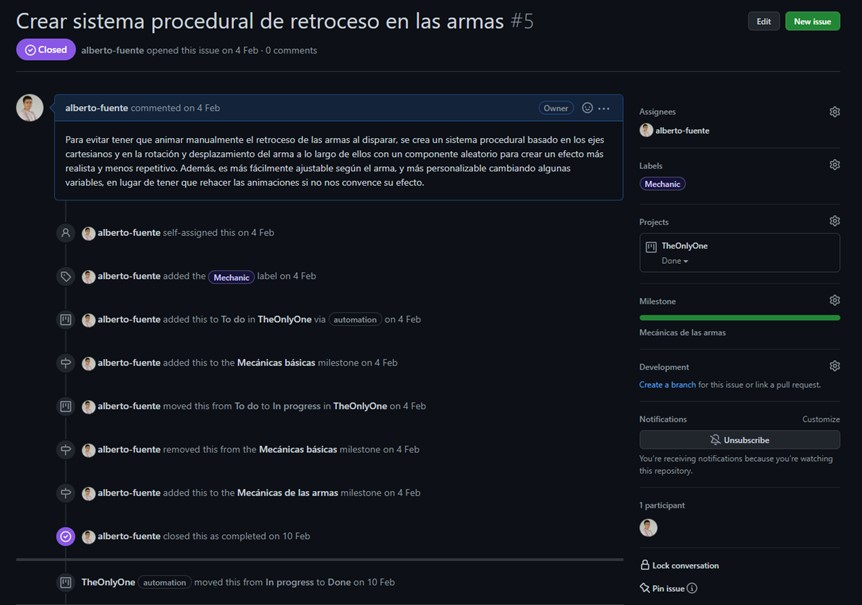
\includegraphics[scale=0.45]{img/GithubScreenshot.jpg}
	\caption{Captura de una tarea en Github}
	\label{fig:TareasGithub}
    \end{figure}
Las tareas representan una acción o pequeño conjunto de acciones relacionadas que han de llevarse a cabo en el proyecto para solventar un problema, crear una mecánica o cumplir un requerimiento. Es decir, son subdivisiones que se hacen del proyecto para poder gestionarlo de forma más eficiente.

Cada tarea se compone de los siguientes elementos:
\begin{itemize}
    \item \textbf{Nombre}: Define en pocas palabras el objetivo de la tarea. 
    \item \textbf{Descripción}: Explica con más detalle en qué consiste la tarea y por qué es necesario teneral en cuenta.
    \item \textbf{Encargado}: Persona o personas que llevarán a cabo la tarea. En este caso, el alumno siempre será el encargado de todas las tareas.
    \item \textbf{Etiquetas}: Se pueden asignar una o varias etiquetas previamente definidas a cada tarea para tener un mejor control sobre ellas y saber de un vistazo a qué ámbito corresponden.\\
    Las etiquetas que se han definido para este proyecto son las siguientes:
    \begin{itemize}
        \item \textbf{Mechanic}. Tarea que forma parte de una mecánica del videojuego. Generalmente se asocia esta etiqueta a aspectos de programación.
        \item \textbf{Animation}. Tareas de animación de algún modelo o interfaz del videojuego.
        \item \textbf{Audio}. Tareas relacionadas con aspectos de sonido o música.
        \item \textbf{Bug}. Algún problema inesperado que requiera solución.
        \item \textbf{Change}. Cambio en algún aspecto o componente del videojuego.
        \item \textbf{Documentation}. Tareas relacionadas con la documentación del proyecto.
        \item \textbf{Enhancement}. Mejoras o nuevas características en algún componente del videojuego.
        \item \textbf{Modelling}. Trabajos de modelado de algún asset del videojuego.
        \item \textbf{UI}. Elementos visuales de la interfaz del usuario como los botones, el HUD o los menús.
        \item \textbf{VFX}. Efectos visuales como partículas o explosiones.
    \end{itemize}
    \item \textbf{Sprint/Milestone/Hito}: Es una agrupación de tareas con una fecha de finalización marcada. En principio, todas las tareas que conforman un sprint deben estar completadas al llegar a dicha marca temporal.\\
    Los sprints suelen ser utilizados en la metodología ágil SCRUM.
\end{itemize}
Los videojuegos son un tipo de proyecto en el que no todas las funcionalidades, mecánicas y contenido del juego están predefinidas antes de comenzar su desarrollo, sino que varias de estas características y apartados irán evolucionando a medida que se vaya desarrollando el juego (quizás porque surjan ideas nuevas, porque se modifiquen otras o porque se tengan que desechar aquellas que parecían buenas en un principio).

La magnitud del proyecto, sumado al hecho de que su desarrollo lo lleva a cabo una única persona, requiere ciclos de revisión rápidos y adaptables que hagan que la comprobación de tareas sea dinámica y flexible y permita una fácil gestión de estas.

Idealmente se debería permitir alargar o acortar la duración de estas si el proyecto así lo requiriese por cualquier motivo, ya que no es raro que los plazos se retrasen, por ejemplo, por culpa de un bug que no permita avanzar en una determinada parte del proyecto.\\ Esto es necesario para reducir al máximo el impacto que el retraso de una tarea pueda provocar al resto del proyecto.

Teniendo en cuenta todos estos factores, se decidió que la planificación temporal de este proyecto se haría a través de la metodología Kanban.

\textbf{\textit{Kanban}} \cite{wiki:Kanban} forma parte de las metodologías ágiles y se basa en el desarrollo y entrega continuos de un pequeño número de tareas de forma fluida y simultánea. Es muy útil en proyectos donde los cambios pueden suceder con facilidad, como es el caso.\\
Además, la metodología Kanban es muy visual, ya que gira en torno a un elemento llamado \textbf{tablero Kanban} (ver figura \ref{fig:TableroKanban}), un conjunto de columnas que conforman espacios para situar las diferentes tareas en función de su grado de completitud, creando un flujo de trabajo en el que se visualiza rápidamente el estado del proyecto.
\begin{figure}[h]
	\centering
	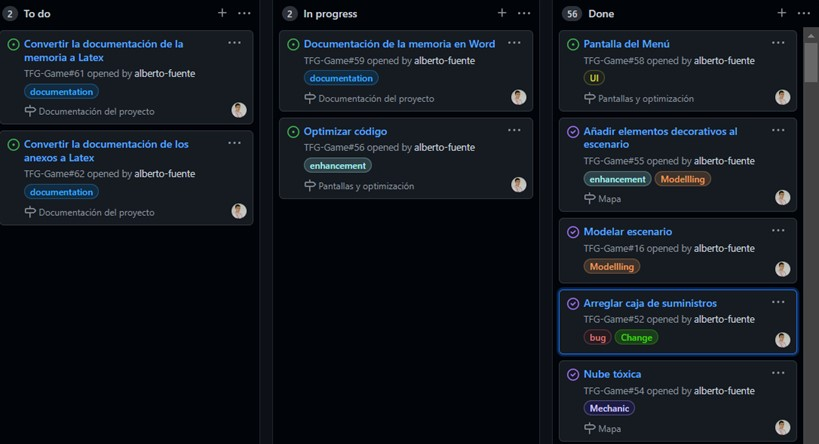
\includegraphics[scale=0.45]{img/KanbanBoard.jpg}
	\caption{Tablero Kanban de Github}
	\label{fig:TableroKanban}
    \end{figure}
Para este proyecto en particular, el tablero Kanban se ha implementado a través de la herramienta de GitHub situada en el apartado ``Projects''. Resulta muy conveniente, ya que se puede asociar el tablero al repositorio del proyecto, de tal manera que cada vez que se crea o modifica el estado de una tarea, aparecerá automáticamente una tarjeta del tablero Kanban.\\
Esto permite trabajar de manera mucho más cómoda y fluida a la hora de gestionar las tareas. 

En este caso, el tablero Kanban está formado por tres columnas y el flujo de estado de las diferentes tareas funciona de la siguiente manera:
\begin{itemize}
    \item \textbf{TO DO}: contiene las tareas que se tiene intención de realizar pero que no han comenzado aún. Cada vez que se crea una nueva tarjeta, se incluirá en esta columna.\\
    Al comienzo del proyecto se incluyen todas las tareas que previsiblemente precisará el proyecto. Sin embargo, algunas pueden ir surgiendo durante su transcurso a medida que se vaya necesitando definir nuevas tareas.
    \item \textbf{IN PROGRESS}: incluye todas las tareas que se están realizando actualmente. El número de tareas en esta columna suele ser reducido, ya que esta metodología prioriza terminar las tareas en curso antes de incorporar otras nuevas.\\ Lo ideal es incluir tareas con un cierto nivel de independencia, es decir, que no estén estrechamente ligadas unas con otras para que un retraso en una de ellas no genere un impacto tan grande en el resto del proyecto.
    \item \textbf{DONE}: contiene las tareas que ya han sido finalizadas. Antes de incluir una tarea en esta columna hay que asegurarse de que la tarea ya ha sido revisada y aquello que abarca funciona adecuadamente.\\
    En el caso de que una tarea interfiriese con otra ya terminada y fuese necesario modificar algún aspecto relacionado con esta última, se crearía una nueva tarea que describiese dicho problema para tenerlo controlado y documentado.
\end{itemize}
 
\subsection{Planificación de los sprints}
Aunque la metodología Kanban es flexible en cuanto a la planificación temporal, conviene marcar unos plazos de tiempo para cuantificar el progreso de cada tarea. Para ello se han empleado los ya mencionados sprints, propios de la metodología SCRUM, a modo de agrupación de tareas y marcando plazos para cada uno de ellos de aproximadamente una semana y media.

Para explicar los sprints que surgieron a lo largo del proyecto se describirán tanto los propios sprints planificados como los distintos \textit{commits} (actualizaciones del Git) que se realizaron durante cada sprint.
\subsubsection{Sprint 1: Mecánicas básicas}
El sprint inicial del proyecto tiene como objetivo implementar las mecánicas esenciales del juego, como el movimiento del jugador y de la cámara. También se pretende añadir las primeras armas (provisionales) al juego para empezar a construir el sistema de disparo y de cambio de armas del jugador.

La fecha marcada para este sprint es el 6 de febrero. Los commits realizados durante este sprint son los siguientes:

\begin{itemize}
    \item \textbf{Actualizar archivo \textit{.gitignore}}: Actualizar el archivo \textit{.gitignore} propio del sistema git para que ignore correctamente los \textit{metafiles} de Unity, aún si están en una subcarpeta.
    \item \textbf{Crear proyecto inicial de Unity}: Crear un proyecto vacío de Unity 3D en el que se trabajará de aquí en adelante.
    \item \textbf{Primeros scripts, modelos provisionales y escenario de pruebas}: Añadir scripts para manejar el movimiento del jugador, la cámara y las armas. Añadir también modelos provisionales de armas y entorno.
    \item \textbf{Mejoras en el sistema de cambio de armas}: Implementar la clase \textit{GrabbableItem}, usada por todos los objetos que pueden ser recogidos por el jugador.
\end{itemize}
\subsubsection{Sprint 2: Mecánicas de las armas}
Implementar el sistema básico de las armas, que engloba tanto la creación de la plantilla para las armas (\textit{Scriptable Object}), como el disparo, la recarga, el apuntado, el retroceso, el cambio de arma y, en general, todo lo relacionado con las armas del juego a nivel programación.
La fecha marcada para este sprint es el 10 de febrero. El único commit realizado durante este sprint fue el siguiente:
\begin{itemize}
    \item \textbf{Crear sistema de recoger y soltar objetos}: Implementar el sistema para recoger y soltar armas y otros objetos del suelo, y arreglar fallos de la clase \textit{GrabbableItem}.
\end{itemize}
\subsection{Sprint 3: Interfaz básica del jugador}
Durante este sprint se comienzan a crear los elementos gráficos que conformarán la interfaz de usuario, así como las diferentes mecánicas asociadas a ellos. Por ejemplo, el HUD de información sobre la munición del arma actual, la vida del jugador, o las etiquetas de los objetos que se encuentre el jugador alrededor del mapa.

La fecha marcada para este sprint es el 18 de febrero. El commit realizado durante este sprint es el siguiente:
\begin{itemize}
    \item \textbf{Crear etiquetas para los objetos}: Crear un sistema de etiquetado de los objetos disponibles para ser recogidos en el mapa para que el usuario pueda ver datos sobre dicho objeto al momento de recogerlo, como su nombre, su rareza o sus estadísticas relevantes. Mejorar algunos aspectos del inventario.
\end{itemize}
\subsection{Sprint 4: Movimiento especial del jugador}
En este sprint se pretenden mejorar las mecánicas de movimiento básicas del jugador, como andar, correr, saltar y mirar alrededor. También se pretende desarrollar algunas mecánicas especiales para el jugador, como el poder deslizarse o correr por las paredes.

La fecha marcada para este sprint es el 3 de marzo. El único commit realizado durante este sprint es el siguiente:
\begin{itemize}
    \item \textbf{Implementar inventario, granadas y corrección de fallos} Se arrastra la implementación del sistema de recogida de objetos del sprint anterior para crear un sistema de inventario para que el jugador pueda llevar varios objetos encima al mismo tiempo. Se crea una interfaz para el inventario. También se añade un nuevo tipo de objeto, las granadas, y se implementa un pequeño HUD para mostrar la munición relativa a las armas equipadas. Se corrigen fallos del anterior sprint.
    \end{itemize}
\subsection{Sprint 5: Sistema de vida y daño del jugador y su interfaz. UI del inventario}
Durante este sprint se pretende Implementar un sistema que controle la vida del jugador en todo momento, haciendo que disminuya cuando recibe daño y que aumente si interactúa con algún tipo de consumible de vida. Crear una interfaz básica de barra de vida para el jugador. También mejorar la interfaz del inventario del jugador para que se ajuste más a la estética general del juego.

La fecha marcada para este sprint es el 17 de marzo. El único commit realizado durante este sprint es el siguiente:
\begin{itemize}
    \item \textbf{UI del inventario y barras de vida y armadura}: Se implementa la interfaz de las barras de vida y de escudo, así como su funcionalidad lógica. Rehacer la interfaz del inventario, acorde con la estética general del videojuego.
\end{itemize}
\subsection{Sprint 6: Redefinición del proyecto}
Este sprint, creado sobre la marcha, tiene como objetivo hacer una redefinición del proyecto, aportando características más concretas acerca del proyecto, teniendo en cuenta la falta de concreción respecto a su alcance. Para ello se rellena un “Documento de Diseño de Videojuegos”. También se debe decidir si el proyecto se sigue desarrollando de manera individual como hasta el momento, o bien en conjunto con el grupo ITACA de la Universidad de Burgos. 

En el apartado ``Aspectos relevantes del proyecto'' de la memoria se explica más a fondo el contexto y desenlace de este sprint.
\subsection{Sprint 7: Programación de enemigos}
En este sprint se tiene como objetivo crear y diseñar la lógica de programación de los enemigos, desde diseñar los diferentes tipos de enemigos que habrá, su comportamiento, inteligencia artificial y estados.

La fecha marcada para este sprint es el 30 de marzo. El único commit realizado durante este sprint es el siguiente:
\begin{itemize}
    \item \textbf{Programación e inteligencia artificial de los enemigos} Implementar la programación básica de los enemigos, como su movimiento, así como su "inteligencia" para detectar tanto al jugador como a otros enemigos con una máquina de estados compuesta por tres estados: deambular, perseguir y atacar.
\end{itemize}
\subsection{Sprint 8: Packs de ayuda para el jugador}
Durante este sprint se busca implementar diferentes tipos de paquetes de ayuda para el jugador, que se dividirán en: Munición, Botiquín, y Armadura, cada uno de los cuales podrá tener cuatro diferentes rarezas: común, rara, épica y legendaria. Según la rareza, el jugador obtendrá más o menos cantidad de dicho paquete. Por ejemplo, los paquetes épicos de munición darán al jugador más munición que los comunes.

La fecha marcada para este sprint es el 7 de abril. El commit realizado durante este sprint es el siguiente:
\begin{itemize}
    \item \textbf{Packs de ayuda para el jugador}: Se han implementado paquetes de munición, salud y armadura, que el jugador podrá recolectar del suelo para regenerar las mismas. Estos paquetes pueden ser de cuatro rarezas cada uno (común, rara, épica y legendaria), en función de la probabilidad de que aparezcan y de sus estadísticas (a mayor rareza, menor probabilidad de aparecer y mejores estadísticas)
\end{itemize}
\subsection{Sprint 8: Sistema de granadas}
En este sprint se desea implementar una nueva mecánica de granadas (compuesta por dos tipos de granadas, aunque abierta a futuras ampliaciones) que el jugador podrá recoger del suelo para arrojarlas a los enemigos. Una es explosiva, hace daño a quien se encuentre dentro de su área de efecto, y la otra es de hielo, congela a los enemigos que se encuentren en su área de congelación. Ambas granadas tienen efectos visuales, sonidos, modelos 3D, texturas, iconos para el inventario y una previsualización de la trayectoria que seguirá la granada al ser lanzada si se presiona el clic derecho del ratón.

La fecha marcada para este sprint es el 17 de abril. El único commit realizado durante este sprint es el siguiente:
\begin{itemize}
    \item \textbf{Sistema de granadas} : Se ha implementado un sistema de granadas, compuesto por dos tipos de granadas que el jugador podrá recoger del suelo para arrojarlas a los enemigos. Una es explosiva, haciendo daño a quien se encuentre dentro de su área de efecto en el momento de la explosión, y la otra es de hielo, congela durante unos segundos a los enemigos que se encuentren en su área de congelación. Ambas granadas tienen efectos visuales, sonidos, modelos 3D, iconos para el inventario.
\end{itemize}
\subsection{Sprint 9: Cajas de equipamiento}
Modelar, animar y programar cajas sorpresa, repartidas por el mapa y que contendrán objetos aleatorios como armas, granadas, o paquetes de ayuda, que el jugador podrá equiparse o consumir para tener más ventaja sobre sus oponentes.

La fecha marcada para este sprint es el 22 de abril. El único commit realizado durante este sprint es el siguiente:
\begin{itemize}
    \item \textbf{Caja de suministros}: Se ha modelado, texturizado, animado y programado una caja de suministros con la que el jugador puede interactuar para conseguir armas nuevas, recargar munición o curarse vida y escudo.
\end{itemize}
\subsection{Sprint 10: Enemigos}
Durante este sprint se procura añadir modelos de los enemigos, animarlos correctamente, programarlos y mejorar su inteligencia.

Añadir modelos 3D a los enemigos, así como las animaciones principales como andar, correr, perseguir o disparar. Mejorar su "inteligencia", corrigiendo errores anteriores, y se han añadido efectos como la explosión de su cabeza si el último disparo recibido antes de morir fue en la cabeza, o la congelación, que afecta a su comportamiento haciendo que se quede inmóvil. Además, cuando un enemigo muere, deja algunos objetos aleatorios en el suelo que pueden ser recogidos por el jugador.

La fecha de finalización marcada para este sprint es el 30 de abril. El único commit realizado durante este sprint es el siguiente:
\begin{itemize}
    \item \textbf{Enemigos}: Se añaden modelos 3D a los enemigos, así como las animaciones principales como andar, correr, perseguir o disparar. Se ha mejorado su "inteligencia", corrigiendo errores anteriores, y se han añadido efectos como la explosión de su cabeza si el último disparo recibido antes de morir fue en la cabeza, o la congelación, que afecta a su comportamiento haciendo que se quede inmóvil. Además, cuando un enemigo muere, deja algunos objetos aleatorios en el suelo que pueden ser recogidos por el jugador.
\end{itemize}
\subsection{Sprint 11: Armas}
En este sprint se persigue el tener todos los componentes de las armas listos. Arreglar errores que pudieran arrastrar de otros sprints, agregar sus animaciones, añadir el modelo de las manos del jugador, así como efectos de sonido y partículas.

La fecha marcada para este sprint es el 10 de mayo. El único commit realizado durante este sprint es el siguiente:
\begin{itemize}
    \item \textbf{Armas y paquetes de ayuda}: Se ha implementado la programación de todas las armas, así como sus diferentes modelos en 3D y animaciones para cada una para las acciones principales, como sacar el arma o recargar. Se han añadido diversos efectos, partículas y sonidos, y se han incorporado brazos al jugador. También se han creado etiquetas renovadas para cada objeto con información relevante del mismo. Además, se han arreglado errores en animaciones de enemigos y en otros aspectos.
\end{itemize}
\subsection{Sprint 12: Mapa}
En este sprint se debe crear el mapa del juego donde se desarrollarán las partidas. Incluye el diseño del terreno, así como los diferentes elementos que irán sobre él, como edificios, decoración, enemigos o cajas de suministro, entre otros.

La fecha marcada para este sprint es el 24 de mayo. El único commit realizado durante este sprint es el siguiente:
\begin{itemize}
    \item \textbf{Generación del mapa y sus elementos}: Se ha implementado un sistema de generación de mapas de manera procedural, así como la colocación aleatoria de edificios, cajas, decoración y enemigos sobre él de manera aleatoria, así como un sistema de daño de manera que el mapa va reduciendo su área segura para acelerar la interacción entre las entidades del juego.
\end{itemize}
\subsection{Sprint 13: Pantallas y optimización}
En este sprint se pretende terminar el diseño final de las pantallas del menú principal, así como las de registro e inicio de sesión de los usuarios. También se pretende optimizar y limpiar el código de todos los scripts creados.

La fecha marcada para este sprint es el 8 de junio. El único commit realizado durante este sprint es el siguiente:

\begin{itemize}
    \item \textbf{Optimización de código y otros arreglos}: Se termina el diseño gráfico de las pantallas del juego, como el menú principal, las pantallas de registro e inicio de sesión, o las de victoria y derrota. Se arreglan algunos bugs ocasionados en sprints anteriores y se optimizan las clases de los scripts para que sean más legibles y facilitar su mantenimiento.
\end{itemize}
\subsection{Sprint 14: Documentación del proyecto}
El sprint final está dedicado a recoger y plasmar toda la documentación del proyecto, incluyendo la memoria y los anexos de este. Para ello se utiliza el sistema Latex \cite{wiki:Latex}, a través de una plantilla de Overleaf \cite{wiki:Overleaf} para tener la jerarquía de apartados ya definida.

\section{Estudio de viabilidad}
Este proyecto no se creó con el objetivo de ser comercializado, sino como un proyecto académico y de aprendizaje personal. Sin embargo, como potencial producto que es, se llevará a cabo un análisis de la viabilidad tanto económica como legal que tendría el proyecto en caso de que fuese distribuido.
\subsection{Viabilidad económica}
Para evaluar si el proyecto tiene viabilidad económica han de valorarse, tanto los costes que suponen el desarrollo del mismo, como los potenciales beneficios que se fueran a obtener dentro de unos plazos marcados.

\subsection{Gastos}
Los gastos que suponen el desarrollo de este proyecto se desglosan a continuación:
\begin{itemize}
    \item \textbf{Costes laborales}: Son los gastos que tiene la empresa al contratar a un trabajador y se componen del salario bruto y las cotizaciones a la Seguridad Social a cargo de la empresa. El salario medio de un programador de videojuegos en España es de 2675€ brutos al mes \cite{wiki:SueldoProgramador}. Las cotizaciones a la Seguridad Social, por otro lado, se dividen a su vez en contingencias comunes (23,60\%), desempleo (5,50\%), formación profesional (0,60\%) y fondo de garantía salarial (FOGASA) (0,20\%) \cite{wiki:SalarioBruto}.
    \item \textbf{Ordenador}: el coste del ordenador utilizado durante el desarrollo del videojuego ha sido de 780€. Teniendo en cuenta que la vida útil del mismo es de 5 años, el coste de amortización mensual será: 780€/5 años/12 meses= 13€/mes.
    \item \textbf{Licencia de Windows 10 Home}: El coste de la licencia del sistema operativo utilizado para el desarrollo del videojuego fue de 145€. Durante los 5 años que se presupone se utilizará el ordenador con la licencia, su coste amortizado mensual será: 145€/5 años/12 meses= 1€/mes.
    \item \textbf{Luz e internet}: 100€ mensuales.
    \item \textbf{Assets de armas}: Los modelos de las armas y granadas utilizadas en el proyecto tuvieron un coste de 5,36€.
    \item \textbf{Impresión de la memoria}: Se calcula que el coste de impresión de la memoria del proyecto ronda los 40€ de coste.
\end{itemize}
Los gastos durante los 4 meses que duró el desarrollo del proyecto se calculan y recogen en la tabla \ref{tab:Gastos del proyecto}:
\begin{table}[t]
\begin{center}
\begin{tabular}{| l | r |}
\hline
\multicolumn{2}{ |c| }{Gastos del proyecto} \\ \hline
\textbf{Concepto} & \textbf{Coste}\\ \hline
Costes laborales &\\
\hspace{1cm}Salario bruto & 2675€ x 4 = 10700€\\
\hspace{1cm}Seguridad Social a cargo de la empresa &\\
\hspace{2cm}·Contingencias comunes (23,60\%) & 631,3€ x 4 = 2525,2€\\
\hspace{2cm}·Desempleo (5,50\%) & 147,125€ x 4 = 588,5€\\
\hspace{2cm}·Formación profesional (0,60\%) & 16,05€ x 4 = 64,2€\\
\hspace{2cm}·FOGASA (0,20\%) & 5,35€ x 4 = 21,4€\\ \hline
Coste amortizado del ordenador & 13€ x 4 = 52€\\\hline
Coste amortizado de la licencia de Windows 10 Home & 1€ x 4 = 4€ \\\hline
Luz e internet & 100€ x 4 = 400€\\\hline
Assets de armas & 5,36€\\\hline
Impresión de la memoria & 40€\\\hline
\textbf{Total} & \textbf{14400,66€}\\\hline
\end{tabular}
\caption{Tabla de gastos del proyecto}
\label{tab:Gastos del proyecto}
\end{center}
\end{table}

\subsection{Ingresos}
Para valorar si el producto puede ser viable económicamente, se tienen que tener en cuenta los ingresos que se obtendrían con el producto una vez lanzado al mercado.

El videojuego se pondría a la venta con un precio de salida de 5€, dada la cantidad de contenido del videojuego y el espectro de precios que suelen tener los juegos \textit{indie} de esta naturaleza.\\
Por lo tanto, para calcular los ingresos se tendría que multiplicar el número de copias vendidas por 5€ de cada copia.

\subsection{Conclusiones}
Con estos datos, para que el juego fuese viable económicamente se tendrían que vender, al menos, \textbf{2881 copias} (14400,66€/5€) . Por lo tanto, si se pretende recuperar la inversión en un año, se tendrían que vender 240 copias al mes (2881 copias/12 meses) o una media de 8 copias al día (240/30). 

Teniendo en cuenta que la mitad de los 6376 juegos indies que se lanzaron en Steam, la principal plataforma de venta de videojuegos, en 2020 no vendieron cada uno más de 640 unidades en total \cite{wiki:VentasVideojuegos} no parece viable económicamente lanzar el juego al mercado con el modelo y las cifras propuestas.

Es posible que, si se llevasen a cabo otras estrategias adicionales, como incluir publicidad en el juego o seguir un modelo Freemium (en el que el juego fuese gratuito, pero con micro transacciones dentro de la aplicación para comprar cosméticos de armas o algún otro elemento estético), este podría tener un mayor éxito y, por tanto, sería finalmente viable económicamente.

\subsection{Viabilidad legal}
Para poder distribuir un producto software como este se deben cumplir ciertos requisitos legales, sobre todo relacionados con las licencias de los diferentes componentes que forman el videojuego.

Los videojuegos, en España, no están reconocidos en la legislación como una obra con naturaleza jurídica propia. Este hecho obliga a registrar de forma individualizada cada elemento del videojuego con el fin de que cumpla con los requisitos legales para considerarse ``obra'' de forma autónoma. \cite{wiki:RequisitosLegales}.

Las licencias de los programas utilizados, como Unity, Blender o Github son gratuitas, y permiten la distribución y comercialización de cualquier producto creado con ellas. Como puntualización, Unity permite comercializar los productos hechos con su motor de manera gratuita siempre que se muestre su logo al inicio del videojuego, algo que está activado por defecto y que no se pretende cambiar.

En cuanto a los assets, la mayoría de los elementos artísticos y scripts han sido creados por el propio desarrollador, lo que le otorga su completa autoría de distribución.

Sin embargo, cabe mencionar algunos elementos que han sido utilizados en el juego y pertenecen a terceros:
\begin{itemize}
    \item La fuente \textit{Hermes}, empleada en varias partes del videojuego, tiene una licencia de uso personal y no comercial si se usa de manera gratuita, como es el caso.
    \item De forma similar, la otra fuente usada en el proyecto, llamada \textit{American Kestrel}, tiene una licencia \textit{freeware} que no permite su uso comercial sin previo pago por ella.
    \item Tanto los modelos de las armas y granadas, como el modelo del robot utilizado en los enemigos no tienen ningún tipo de licencia descrita por los creadores, pero dado que se obtuvieron desde la tienda de assets de unity, el producto se rige bajo la licencia \textbf{\textit{Standard Unity Asset Store End User License Agreement}(EULA)}  en la que se describe que todos los productos de la tienda de Unity pueden usarse con una finalidad comercial.
    \item La mayoría de sonidos utilizados en el juego se descargaron de una librería de sonidos llamada \textit{Epidemic Sound} a través de una prueba gratuita. Durante dicha prueba, la librería otorga todos los derechos de distribución, comercialización y monetización del material utilizado.\\ 
    Sin embargo, al finalizar el período de prueba, se pierden los derechos comerciales, quedando únicamente el derecho al uso personal de los mismos.
\end{itemize}
Por lo tanto, si se quisiese comercializar el juego, se tendrían que pagar las licencias de uso comercial de las fuentes, así como reactivar la suscripción a la librería de sonidos de \textit{Epidemic Sound}.

En este caso, como no se pretende comercializar el videojuego creado, se elegiría marcar el producto bajo la licencia \textbf{\textit{Creative Commons}}, más concretamente del tipo \textbf{CC-BY-NC-ND 4.0}. \cite{wiki:Licencia}, la más restrictiva de todas, y que permite que otros puedan descargar y compartir el producto con otras personas en cualquier medio o formato, siempre que se reconozca la autoría del producto y que no se modifique ningún aspecto del juego ni se comercialice.
\apendice{Especificación de Requisitos}

\section{Introducción}
En este apartado se detallarán todos los requisitos, tanto funcionales como no funcionales, que tiene que cumplir el producto para abarcar los objetivos iniciales propuestos, es decir, se comprobará si las funcionalidades del producto cumplen con lo esperado.
\section{Objetivos generales}
Los objetivos que se desean alcanzar con el desarrollo del proyecto son los siguientes:
\begin{itemize}
\tightlist
	\item Desarrollar un videojuego de género \textit{shooter}, en concreto del estilo \textit{battle royale}, para ordenador como plataforma de juego, compatible con Windows y Linux y pensado para controlarse con teclado y ratón. Este objetivo puede subdividirse a su vez en objetivos más concretos:
    	\begin{itemize}
    	\tightlist
    	\item Desarrollar una buena \textbf{jugabilidad} y mecánicas interesantes para que el producto resulte entretenido y divertido para los usuarios.
    	\item Hacer que el producto sea \textbf{accesible} para un gran espectro de usuarios, es decir, que aprendan las mecánicas y acciones que ofrece el videojuego de forma intuitiva y con una curva de aprendizaje sencilla y no frustrante.
    	\item Crear de manera \textbf{autónom}a la mayoría de componentes del videojuego, incluyendo scripts, modelos, texturas, efectos, elementos de interfaces y sonidos.
    	\item Hacer que el videojuego sea \textbf{óptimo} en términos de rendimiento.
    	\item Utilizar \textbf{patrones, algoritmos y estructuras} de programación convenientes en cada caso.
    	\item Hacer que el proyecto sea fácilmente \textbf{extensible} para incluir mecánicas, objetos, mejoras o modificaciones de manera sencilla e intuitiva.
    	\end{itemize}
	\item Aprender el funcionamiento y las características fundamentales de Unity, así como del lenguaje de programación que utiliza (C\#)
	\item Aplicar la metodología \textit{Kanban} durante el desarrollo del producto para la gestión de las tareas.
	\item Integrar Git y Github como sistema de control de versiones.
	\item Asentar las bases de conocimiento personal para poder realizar otros proyectos similares en el futuro o continuar el desarrollo y mejora del mismo.
\end{itemize}
\section{Catalogo de requisitos}
En este apartado se detallarán cada uno de los requisitos del producto. Estos se pueden dividir, dependiendo de su naturaleza, en dos categorías: \textbf{funcionales} y \textbf{no funcionales}.

\subsection{Requisitos funcionales}
Son los servicios y funciones que el sistema debe ofrecer ante la interacción de los usuarios con él.
\begin{itemize}
    \item \textbf{RF-1 Iniciar sesión}: El jugador debe poder ser identificado de manera única e inequívoca para diferenciarse de los demás jugadores existentes en la aplicación y acceder a su cuenta.
    \begin{itemize}
        \item \textbf{RF-1.1 Registro}: El usuario debe poder registrarse en el juego introduciendo sus datos como nombre de usuario, correo y contraseña para crear una cuenta.
    \end{itemize}
    \item \textbf{RF-2 Gestión del menú principal}: Debe haber un menú central desde el que se pueda navegar a las distintas secciones de la aplicación.
    \begin{itemize}
        \item \textbf{RF-2.1 Mostrar datos del jugador}: El jugador debe poder ver su nombre de usuario y su experiencia total en el menú principal.
        \item \textbf{RF-2.2 Gestión del Menú de opciones}: El jugador debe poder acceder a un menú de opciones generales del juego y así poder modificar algunos aspectos generales del juego como la resolución, la calidad gráfica o el volumen del sonido.
        \item \textbf{Ver Clasificación}: El jugador debe poder ver quiénes son los jugadores que más experiencia han acumulado en el juego en forma de lista, actualizándose esta cada vez que se consulte.
        \item \textbf{RF-2.4 Cerrar sesión}: El jugador debe poder cerrar su sesión de usuario.
        \item \textbf{RF-2.5 Salir del juego}: El jugador debe poder salir de la aplicación cuando lo desee.
    \end{itemize}
    \item \textbf{RF-3 Jugar}: El sistema debe permitir iniciar y desarrollar una partida.
    \begin{itemize}
        \item \textbf{RF-3.1 Generación de mapa}: El juego debe ser capaz de generar un mapa al inicio de la partida de forma procedural y única en cada partida.
        \item \textbf{RF-3.2 Mover al jugador}: El jugador debe poder moverse en cualquier dirección sobre el terreno, según el input que se reciba del usuario.
        \begin{itemize}
            \item \textbf {RF-3.2.1 Deslizarse}: El jugador debe poder deslizarse por el terreno si así lo desea y si el terreno es lo suficientemente inclinado
            \item \textbf{RF-3.2.2 Correr por la pared}: el jugador debe poder correr por las paredes y saltar desde ellas a otras paredes para moverse de manera más dinámica y que pueda alcanzar lugares altos de difícil acceso.
        \end{itemize}
        \item \textbf{RF-3.3 Mirar alrededor}: El jugador debe poder mirar a su alrededor, dirigiendo la mirada donde el usuario desee.
        \item \textbf{RF-3.4 Saltar}: El jugador debe poder saltar, elevándose en el aire.
        \begin{itemize}
            \item \textbf{RF-3.4.1 Usar trampolín}: El jugador debe poder saltar sobre una plataforma de rebote que le impulse varios metros en el aire para llegar a lugares altos o huir de algún sitio.
        \end{itemize}
        \item \textbf{RF3.5 Abrir caja de suministros}: El jugador debe poder abrir las cajas de suministros que encuentre.
        \item \textbf{RF3.6 Equipar armamento}: El jugador debe poder equipar y añadir a su inventario objetos de armamento que encuentre en cajas o en el suelo, como armas o granadas, hasta poder llenarlo por completo.
        \item \textbf{RF-3.7 Desequipar armamento}: El jugador debe poder desequipar el objeto que desee de entre los que tenga equipados en el inventario.
        \item \textbf{RF-3.8 Cambiar armamento activo}: El jugador debe poder elegir qué objeto del armamento tener activo en cada momento.
        \item \textbf{RF3.9 Utilizar armamento}: El jugador debe poder utilizar el armamento que tenga equipado en el inventario.
        \begin{itemize}
            \item \textbf{RF3.9.1 Disparar arma}: El jugador debe poder disparar el arma que tenga equipada en ese momento.
            \item \textbf{RF3.9.2 Lanzar granada}: El jugador debe poder lanzar la granada que tenga equipada en ese momento.
            \item \textbf{RF3.9.3 Recargar arma}: El jugador debe poder recargar el arma que tenga equipada en ese momento.
            \item \textbf{RF3.9.4 Apuntar}: El jugador debe poder apuntar con el arma o la granada que tenga equipada en ese momento.
        \end{itemize}
        \item \textbf{RF3.10 Consumir packs de ayuda}: El jugador debe ser capaz de utilizar y consumir diferentes paquetes de ayuda que se encuentre por el mapa.
        \begin{itemize}
            \item \textbf{RF3.10.1 Consumir pack de vida}: El jugador debe ser capaz de recuperar cierta cantidad de salud al consumir un pack de vida. En función de su rareza, recuperará más o menos vida.
            \item \textbf{RF3.10.2 Consumir pack de armadura}: El jugador debe ser capaz de recuperar cierta cantidad de armadura al consumir un pack de armadura. En función de su rareza, recuperará más o menos armadura.
            \item \textbf{RF3.10.3 Consumir pack de munición}: El jugador debe ser capaz de rellenar los cargadores de las armas que tenga equipadas al consumir un pack de munición. En función de su rareza, recibirá más o menos cargadores.
        \end{itemize}
        \item \textbf{RF-3.11 Interacción con enemigos}: El jugador debe poder interactuar de manera recíproca con los enemigos que encuentre durante la partida.
        \begin{itemize}
            \item \textbf{RF3.11.1 Ataque entre enemigos}: Los enemigos deben poderse disparar ente ellos para hacerse daño e incluso eliminarse.
            \item \textbf{RF3.11.2 Ataque al enemigo}: El jugador debe poder atacar y hacer daño a los enemigos para reducir su vida.
            \item \textbf{RF3.11.3 Matar enemigo}: El jugador debe poder matar a los enemigos.
        \end{itemize}
        \item \textbf{RF-3.12 Recibir daño}: El jugador debe poder recibir daño de diversas fuentes, como enemigos, granadas o por estar dentro de la nube tóxica.
        \item \textbf{RF3.13 Interacción con nube tóxica}: El juego debe disponer de una nube tóxica que delimitará el espacio seguro del mapa, fuera del cual el jugador y el resto de entidades perderán vida progresivamente. El espacio seguro se irá reduciendo a medida que avance la partida.
        \item \textbf{RF 3.14 Gestión de la interfaz}: El juego debe poder actualizar los elementos gráficos de HUD y sus valores de acorde a lo que ocurra en el juego. Estos elementos son el inventario, las barras de vida y armadura, los valores que indican cuántas entidades quedan vivas y cuántas ha eliminado el jugador, pantallas de cura, armadura y daño, o la munición actual del jugador.
        \item \textbf{RF-3.15 Pausar la partida}: El jugador debe poder poner en estado de pausa la partida en cualquier momento durante su transcurso y volver a reanudarla cuando lo desee.
        \item \textbf{RF-3.16 Salir de la partida}: El jugador debe poder abandonar la partida en cualquier momento, volviendo al menú principal del juego.
        \item \textbf{RF-3.17 Ganar la partida}: El jugador debe poder conseguir la victoria si es el único superviviente de la partida. 
        \item \textbf{RF-3.18 Morir}: El jugador debe poder morir y por tanto perder la partida
    \end{itemize}
\end{itemize}

\subsection{Requisitos no funcionales}
Todo producto software que vaya a ser utilizado por una o varias personas precisa de ciertos requisitos no funcionales para asegurar la calidad del mismo y, este, al ser un videojuego, requiere que estos se cumplan de manera más firme para que el jugador tenga una experiencia de juego satisfactoria.
\begin{itemize}
    \item \textbf{RNF-1 Usabilidad}: la intención de este videojuego es que sea fácil de usar y que su curva de aprendizaje sea sencilla y rápida, para evitar que los jugadores se frustren si resulta demasiado complicado jugar. Los jugadores deben divertirse a la vez que aprenden todas las mecánicas que el videojuego le ofrece hasta llegar a controlarlas a un nivel básico y suficiente para poder divertirse y ganar algunas partidas antes de poder dominarlo por completo.
    \item \textbf{RFN-2 Experiencia y Look and feel}: Ofrecer una experiencia inmersiva en la que el jugador durante la sesión de juego, se adentre en el mundo virtual y sienta que de verdad encarna al protagonista del videojuego y que tiene que luchar para mantenerse con vida.
    
    Se pretende que sea agradable navegar por los menús, que la estética sea coherente, la ambientación y distintos elementos sean los adecuados, la iluminación y sonido estén bien integrados, las mecánicas sean fluidas y se comporten como el jugador lo espera. Uno de los objetivos prioritarios que se pretende mantener con cada elemento añadido al sistema es el llamado \textit{Game Feel}.\\
    \textbf{\textit{Game Feel}} es un término que se refiere a cómo se siente utilizar el juego. La sensación física de que, por ejemplo, utilizar una pistola y un francotirador se sienta diferente. Que la pistola se sienta ligera, débil y rápida, mientras que el francotirador sea lento, pesado pero potente. Que el personaje responda como debe al input del usuario, obteniendo movimientos fluidos y naturales que aporten sensación de control. Que surjan partículas del suelo cuando el jugador aterriza en él, que la información de un objeto aparezca cuando el jugador dirige la mirada hacia él o que aparezcan efectos de pantalla cuando el jugador recibe daño o se cura.
    
    Todos ellos son elementos y detalles que mejoran este \textit{Game Feel}, haciendo que cada acción que sucede sea más interesante y agradable, lo que marca la diferencia entre un buen y un mal videojuego.

    \item \textbf{RNF-3 Escalabilidad}: El videojuego debe responder con la mayor facilidad posible ante las posibles extensiones del mismo que surjan con nuevas mecánicas y funcionalidades que se quieran añadir, es decir, debe ser fácilmente escalable a lo largo del tiempo haciendo que añadir contenido futuro al videojuego sea una tarea sencilla, intuitiva, y su adaptación a la aplicación sea lo más fluida posible.\\
    Es por ello que, tanto el código como el resto de la arquitectura de la aplicación, debe ser fácil de comprender, mantener y extender.
    \item \textbf{RFN-4 Universalidad}: El videojuego está diseñado para que pueda ser jugado por un público muy amplio, desde adolescentes hasta personas de mediana edad. Además, los modelos y la estética del videojuego son \textit{Mid-poly}, siendo algunos \textit{Low-poly}, orientado a que la aplicación está optimizada para poder ser ejecutada incluso sobre ordenadores de gama media-baja con unas prestaciones computacionales no muy elevadas sin que se alarguen demasiado los tiempos de carga ni haya ralentizaciones de frames. Además, se incluyen opciones de calidad gráfica para que se asegure la fluidez de juego en la mayoría de dispositivos, y de esta manera, atraiga a más jugadores.
    \item \textbf{RFN-5 Soporte multiplataforma}: La aplicación debe poder ejecutarse correctamente en varios sistemas operativos, como Windows y Linux, y debe ser fácilmente adaptable a otras plataformas y soportes si se requiriese en un futuro. Una de las razones por la que se escogió el motor Unity para realizar este videojuego fue su fácil compilación y distribución en diversas plataformas de juego.
\end{itemize}

\section{Especificación de requisitos}
En este apartado se analizará cada uno de los casos de uso principales de la aplicación, así como un diagrama que resuma la interacción entre ellos y el actor del sistema.

\subsection{Diagrama de casos de uso}
En la figura \ref{fig:CasosdeUso} se puede observar el diagrama de casos de uso de la aplicación.
\begin{figure}[h]
	\centering
	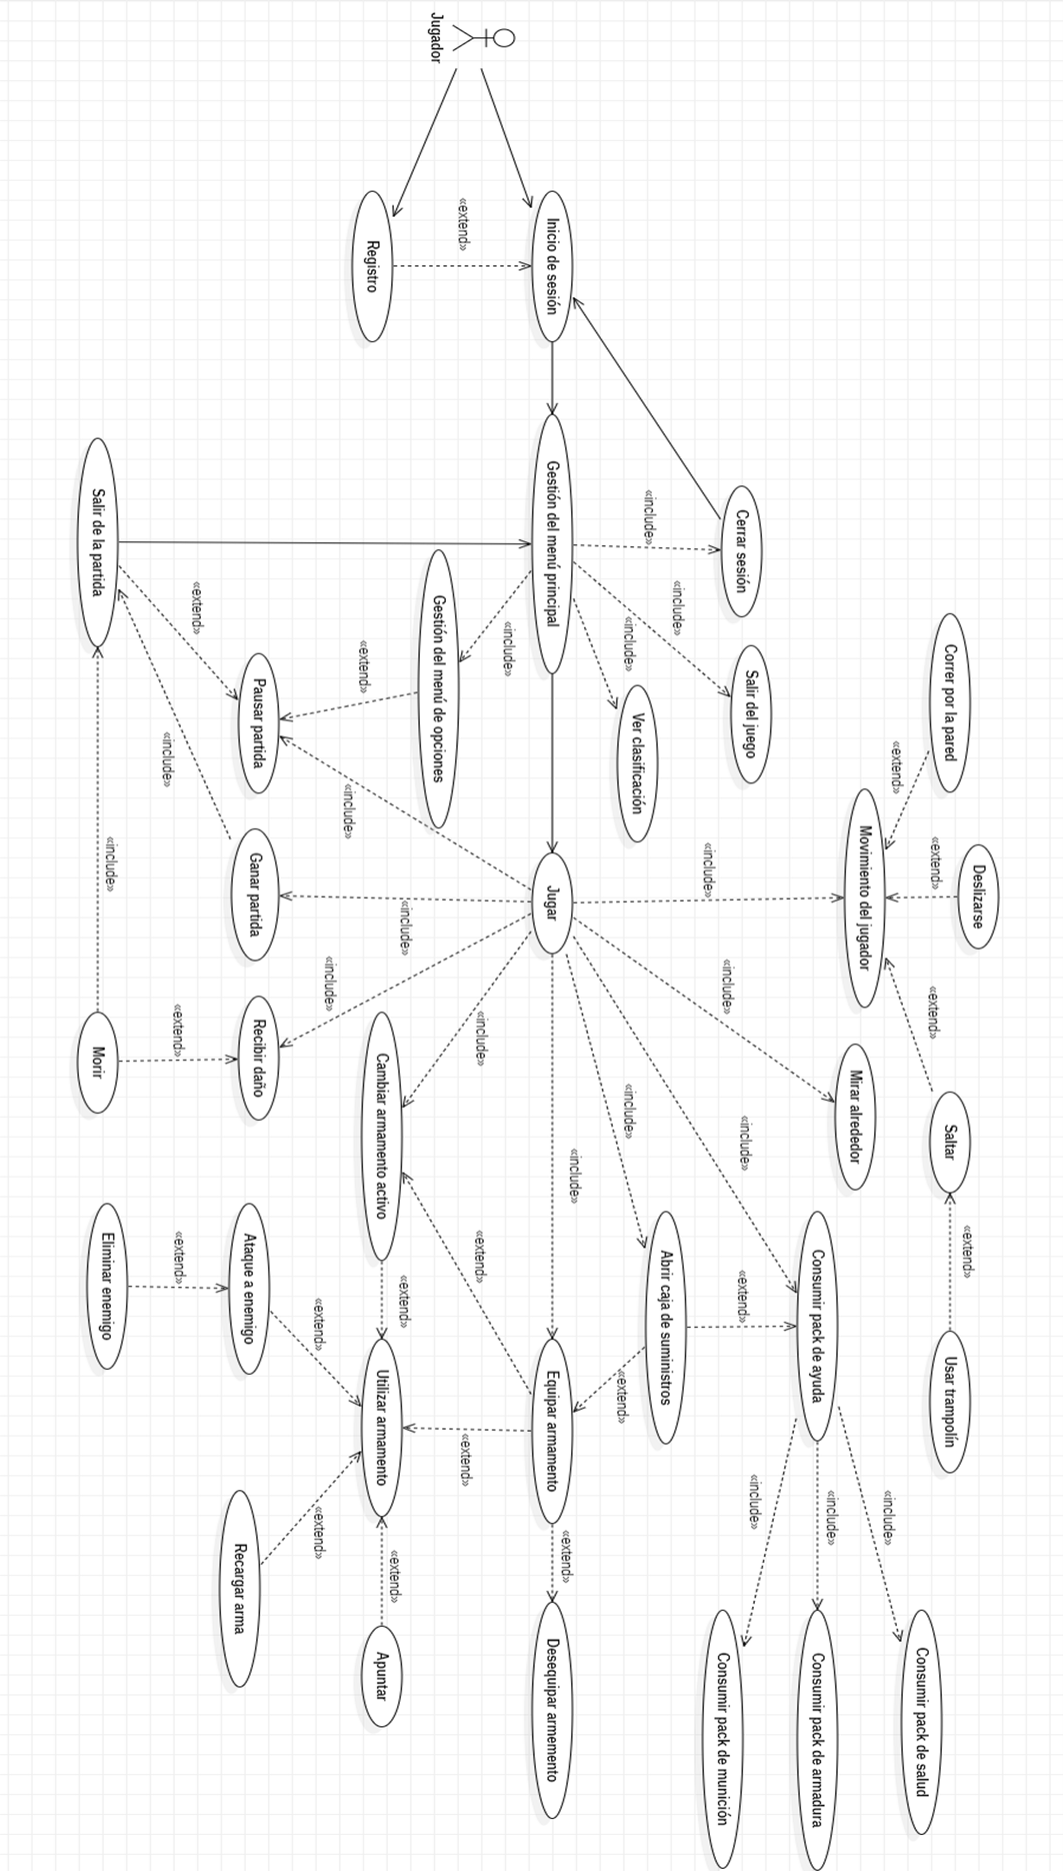
\includegraphics[scale=0.4]{img/UseCaseDiagram.png}
	\caption{Diagrama de casos de uso}
	\label{fig:CasosdeUso}
    \end{figure}
    
\subsection{Actores}
Al ser un videojuego en el que participa un solo jugador, el único actor del sistema será el propio jugador.

\subsection{Casos de Uso}
\tablaSmallSinColores{CU-01: Iniciar sesión}{p{3cm} p{.75cm} p{10cm}}{tablaCU1}{
	\multicolumn{3}{p{10.25cm}}{Caso de uso 1: Iniciar sesión} \\
}
{   
	Descripción                            & \multicolumn{2}{p{10.25cm}}{Permite al usuario de la aplicación identificarse de manera única e inequívoca para diferenciarse de los demás jugadores existentes y acceder a su cuenta.} \\\hline
	Requisitos                         	   & \multicolumn{2}{p{10.25cm}}{RF-1} \\\hline
	Precondiciones                         & \multicolumn{2}{p{10.25cm}}{Haber iniciado la aplicación y haber introducido las credenciales correctas del jugador} \\\hline

	\multirow{3}{2cm}{Secuencia normal}  & Paso & Acción \\\cline{2-3}
	& 1    & El usuario inicia el videojuego. \\\cline{2-3}
	& 2    & El usuario introduce sus credenciales (correo y contraseña). \\\cline{2-3}
	& 3    & El usuario pulsa en el botón ``Iniciar sesión''. \\\hline
	Postcondiciones                        & \multicolumn{2}{p{10.25cm}}{Se muestra el menú principal con algunos datos del usuario} \\\hline
	Excepciones                            & \multicolumn{2}{p{10.25cm}}{El usuario introduce las credenciales incorrectas, el sistema le avisa y puede introducirlas de nuevo. El usuario no está registrado. El usuario  sale de la aplicación.
}\\\hline
	Frecuencia                             & \multicolumn{2}{p{4cm}}{Baja} \\\hline
	Importancia                            & \multicolumn{2}{p{4cm}}{Muy alta} \\\hline

}
\tablaSmallSinColores{CU-2: Registrarse}{p{3cm} p{.75cm} p{10cm}}{tablaCU2}{
\multicolumn{3}{p{10.25cm}}{Caso de uso 2: Registrarse} \\
}
{   
Descripción                            & \multicolumn{2}{p{10.25cm}}{El usuario se da de alta en el juego para que empiece a registrar sus estadísticas} \\\hline
Requisitos                           & \multicolumn{2}{p{10.25cm}}{RF-1, RF-1-1} \\\hline
Precondiciones                         & \multicolumn{2}{p{10.25cm}}{Haber pulsado el botón “Registrarse” en la pantalla de identificación y haber introducido datos válidos} \\\hline

\multirow{3}{2cm}{Secuencia normal}  & Paso & Acción \\\cline{2-3}
& 1    & El usuario pulsa en “Registrarse”. \\\cline{2-3}
& 2    & El usuario introduce sus datos, como el nombre de usuario, el correo y la contraseña \\\cline{2-3}
& 3    & El usuario pulsa en “Registrarse”. \\\hline
Postcondiciones                        & \multicolumn{2}{p{10.25cm}}{El usuario puede iniciar sesión con su correo y contraseña} \\\hline
Excepciones                            & \multicolumn{2}{p{10.25cm}}{El usuario introduce algún dato inválido, el sistema le avisa y puede introducirlo de nuevo. El usuario vuelve a la pantalla de identificación sin terminar el registro}\\\hline
Frecuencia                             & \multicolumn{2}{p{4cm}}{Muy baja} \\\hline
Importancia                            & \multicolumn{2}{p{4cm}}{Muy alta} \\\hline

}


\tablaSmallSinColores{CU-3: Gestión del menú principal}{p{3cm} p{.75cm} p{10cm}}{tablaCU3}{
\multicolumn{3}{p{10.25cm}}{Caso de uso 3: Gestión del menú principal} \\
}
{   
Descripción                            & \multicolumn{2}{p{10.25cm}}{El usuario se encuentra en un menú donde puede escoger la acción que desee en relación con el juego, al tiempo que ve su nombre de usuario y su experiencia total actual} \\\hline
Requisitos                           & \multicolumn{2}{p{10.25cm}}{ RF-2, RF-2.1, RF-2.2, RF-2.3, RF-2.4, RF-2.5} \\\hline
Precondiciones                         & \multicolumn{2}{p{10.25cm}}{ El usuario debe haber iniciado sesión con éxito} \\\hline

\multirow{3}{2cm}{Secuencia normal}  & Paso & Acción \\\cline{2-3}
& 1    & El usuario accede al menú. \\\cline{2-3}
& 2    & El sistema muestra todas las acciones disponibles para el usuario. \\\cline{2-3}
& 3    & El usuario marca el botón de su elección. \\\cline{2-3}
& 4    & El sistema responde de acuerdo con la acción marcada \\\hline
Postcondiciones                        & \multicolumn{2}{p{10.25cm}}{Dependiendo de la opción elegida, el sistema tomará las acciones necesarias para responder la petición del usuario} \\\hline
Excepciones                            & \multicolumn{2}{p{10.25cm}}{El usuario pulsa la acción de “Salir” y la aplicación se cierra, terminando la secuencia del programa}\\\hline
Frecuencia                             & \multicolumn{2}{p{4cm}}{Baja} \\\hline
Importancia                            & \multicolumn{2}{p{4cm}}{Alta} \\\hline

}
\tablaSmallSinColores{CU-4: Jugar}{p{3cm} p{.75cm} p{10cm}}{tablaCU4}{
\multicolumn{3}{p{10.25cm}}{Caso de uso 4: Jugar} \\
}
{   
Descripción                            & \multicolumn{2}{p{10.25cm}}{El usuario selecciona la opción “jugar” en el menú principal para comenzar una partida} \\\hline
Requisitos                           & \multicolumn{2}{p{10.25cm}}{RF-3, RF-3.1, RF-3.2, RF-3.3, RF-3.4, RF-3.5, RF-3.6, RF-3.7, RF-3.8, RF-3.9, RF-3.10} \\\hline
Precondiciones                         & \multicolumn{2}{p{10.25cm}}{ El usuario debe haber pulsado el botón “Jugar” en el menú principal} \\\hline

\multirow{3}{2cm}{Secuencia normal}  & Paso & Acción \\\cline{2-3}
& 1    & El jugador pulsa “jugar” en el menú principal. \\\cline{2-3}
& 2    & El sistema muestra una pantalla de carga mientras construye el terreno y sus elementos. \\\cline{2-3}
& 3    & El jugador aparece en el mapa y puede empezar la partida. \\\hline
Postcondiciones                        & \multicolumn{2}{p{10.25cm}}{El jugador empieza la partida} \\\hline
Excepciones                            & \multicolumn{2}{p{10.25cm}}{-}\\\hline
Frecuencia                             & \multicolumn{2}{p{4cm}}{Baja} \\\hline
Importancia                            & \multicolumn{2}{p{4cm}}{Muy alta} \\\hline

}

\tablaSmallSinColores{CU-5: Movimiento del jugador}{p{3cm} p{.75cm} p{10cm}}{tablaCU5}{
\multicolumn{3}{p{10.25cm}}{Caso de uso 5: Movimiento del jugador} \\
}
{   
Descripción                            & \multicolumn{2}{p{10.25cm}}{El jugador se mueve por el terreno del mapa en la dirección deseada.} \\\hline
Requisitos                           & \multicolumn{2}{p{10.25cm}}{ RF-3, RF-3.2} \\\hline
Precondiciones                         & \multicolumn{2}{p{10.25cm}}{Haber comenzado una partida} \\\hline

\multirow{3}{2cm}{Secuencia normal}  & Paso & Acción \\\cline{2-3}
& 1    & El usuario presiona las teclas “W” (adelante), “S” (atrás), “A” (izquierda) o “D” (Derecha), según la dirección en la que se quiera mover. Opcionalmente puede mantener pulsada la tecla “shift” para correr. \\\hline
Postcondiciones                        & \multicolumn{2}{p{10.25cm}}{El jugador se desplaza hacia un determinada dirección según las teclas pulsadas.} \\\hline
Excepciones                            & \multicolumn{2}{p{10.25cm}}{El usuario no presiona ninguna tecla y el jugador no se mueve}\\\hline
Frecuencia                             & \multicolumn{2}{p{4cm}}{Muy alta } \\\hline
Importancia                            & \multicolumn{2}{p{4cm}}{Alta} \\\hline

}
\tablaSmallSinColores{CU-6: Deslizarse}{p{3cm} p{.75cm} p{10cm}}{tablaCU6}{
\multicolumn{3}{p{10.25cm}}{Caso de uso 6: Deslizarse} \\
}
{   
Descripción                            & \multicolumn{2}{p{10.25cm}}{El jugador se desliza por el terreno cuando está lo suficientemente inclinado} \\\hline
Requisitos                           & \multicolumn{2}{p{10.25cm}}{RF-3, RF-3.2, RF-3.2.1} \\\hline
Precondiciones                         & \multicolumn{2}{p{10.25cm}}{ El jugador tiene los pies apoyados sobre el suelo} \\\hline

\multirow{3}{2cm}{Secuencia normal}  & Paso & Acción \\\cline{2-3}
& 1    & El usuario presiona la tecla “Ctrl” (Control) y opcionalmente también alguna tecla de dirección para dirigir mejor el movimiento. \\\cline{2-3}
& 2    & El jugador, si se encuentra sobre un terreno inclinado hacia abajo, se desliza por él. \\\hline
Postcondiciones                        & \multicolumn{2}{p{10.25cm}}{El jugador se desplaza rápidamente hacia una zona más baja del mapa} \\\hline
Excepciones                            & \multicolumn{2}{p{10.25cm}}{No hay suficiente pendiente para deslizarse }\\\hline
Frecuencia                             & \multicolumn{2}{p{4cm}}{Media } \\\hline
Importancia                            & \multicolumn{2}{p{4cm}}{Media} \\\hline

}
\tablaSmallSinColores{CU-7: Correr por la pared}{p{3cm} p{.75cm} p{10cm}}{tablaCU7}{
\multicolumn{3}{p{10.25cm}}{Caso de uso 7: Correr por la pared} \\
}
{   
Descripción                            & \multicolumn{2}{p{10.25cm}}{El jugador puede adherirse a una pared para correr sobre ella y saltar desde la pared a otras paredes cercanas, creando un efecto de escalada alterno.} \\\hline
Requisitos                           & \multicolumn{2}{p{10.25cm}}{RF-3, RF-3.2, RF-3.2.2} \\\hline
Precondiciones                         & \multicolumn{2}{p{10.25cm}}{Debe haber una pared junto al jugador} \\\hline

\multirow{3}{2cm}{Secuencia normal}  & Paso & Acción \\\cline{2-3}
& 1    & El usuario salta junto a una pared. \\\cline{2-3}
& 2    & El jugador automáticamente se adhiere a dicha pared. \\\cline{2-3}
& 3    & Mientras tenga la tecla de dirección que apunta a la pared presionada, el jugador se mantiene adherido. \\\cline{2-3}
& 4    & El jugador presiona avanza por la pared presionando la tecla de dirección “W”. \\\cline{2-3}
& 5    & El jugador puede saltar en dirección opuesta a la pared presionando la tecla de salto “Espacio” y poder alcanzar un sitio más alto \\\hline
Postcondiciones                        & \multicolumn{2}{p{10.25cm}}{El jugador puede repetir esta acción en paredes cercanas para crear un efecto de escalada} \\\hline
Excepciones                            & \multicolumn{2}{p{10.25cm}}{ El usuario deja de presionar la tecla de dirección correcta y se baja de la pared}\\\hline
Frecuencia                             & \multicolumn{2}{p{4cm}}{Media} \\\hline
Importancia                            & \multicolumn{2}{p{4cm}}{Media} \\\hline

}
\tablaSmallSinColores{CU-8: Mirar alrededor }{p{3cm} p{.75cm} p{10cm}}{tablaCU8}{
\multicolumn{3}{p{10.25cm}}{Caso de uso 8: Mirar alrededor} \\
}
{   
Descripción                            & \multicolumn{2}{p{10.25cm}}{El jugador gira su cabeza para mirar el entorno y los objetos de su alrededor} \\\hline
Requisitos                           & \multicolumn{2}{p{10.25cm}}{RF-3, RF-3.3} \\\hline
Precondiciones                         & \multicolumn{2}{p{10.25cm}}{Haber comenzado una partida} \\\hline

\multirow{3}{2cm}{Secuencia normal}  & Paso & Acción \\\cline{2-3}
& 1    & El usuario desplaza el ratón en la dirección hacia la que quiera dirigir la mirada del jugador. \\\cline{2-3}
& 2    & El jugador gira su cabeza. \\\hline
Postcondiciones                        & \multicolumn{2}{p{10.25cm}}{El jugador puede ver la parte del entorno correspondiente} \\\hline
Excepciones                            & \multicolumn{2}{p{10.25cm}}{ El jugador no mueve el ratón y siempre verá la misma región}\\\hline
Frecuencia                             & \multicolumn{2}{p{4cm}}{Muy alta} \\\hline
Importancia                            & \multicolumn{2}{p{4cm}}{Alta} \\\hline

}
\tablaSmallSinColores{CU-9: Salto del jugador}{p{3cm} p{.75cm} p{10cm}}{tablaCU9}{
\multicolumn{3}{p{10.25cm}}{Caso de uso 9: Salto del jugador} \\
}
{   
Descripción                            & \multicolumn{2}{p{10.25cm}}{El jugador se eleva en el aire unos instantes} \\\hline
Requisitos                           & \multicolumn{2}{p{10.25cm}}{RF-3, RF-3.4} \\\hline
Precondiciones                         & \multicolumn{2}{p{10.25cm}}{El jugador tiene los pies apoyados en alguna superficie} \\\hline

\multirow{3}{2cm}{Secuencia normal}  & Paso & Acción \\\cline{2-3}
& 1    & El usuario presiona la tecla “Espacio”. \\\cline{2-3}
& 2    & El jugador salta. \\\hline
Postcondiciones                        & \multicolumn{2}{p{10.25cm}}{El jugador vuelve a caer por el efecto de la gravedad.} \\\hline
Excepciones                            & \multicolumn{2}{p{10.25cm}}{ El jugador ya se encuentra en el aire}\\\hline
Frecuencia                             & \multicolumn{2}{p{4cm}}{Media} \\\hline
Importancia                            & \multicolumn{2}{p{4cm}}{Baja} \\\hline

}
\tablaSmallSinColores{CU-10: Usar trampolín}{p{3cm} p{.75cm} p{10cm}}{tablaCU10}{
\multicolumn{3}{p{10.25cm}}{Caso de uso 10: Usar trampolín} \\
}
{   
Descripción                            & \multicolumn{2}{p{10.25cm}}{El jugador se impulsa varios metros en el aire, haciendo que pueda alcanzar lugares muy altos o que pueda escapar de algún sitio rápidamente} \\\hline
Requisitos                           & \multicolumn{2}{p{10.25cm}}{RF-3, RF-3.4, RF-3.4.1} \\\hline
Precondiciones                         & \multicolumn{2}{p{10.25cm}}{El jugador tiene se encuentra sobre una plataforma de salto} \\\hline

\multirow{3}{2cm}{Secuencia normal}  & Paso & Acción \\\cline{2-3}
& 1    & El usuario se sitúa sobre una plataforma de salto. \\\cline{2-3}
& 2    & El usuario presiona la tecla “Espacio”. \\\cline{2-3}
& 3    & El sistema eleva al jugador varios metros en el aire. \\\hline
Postcondiciones                        & \multicolumn{2}{p{10.25cm}}{El jugador vuelve a caer por el efecto de la gravedad} \\\hline
Excepciones                            & \multicolumn{2}{p{10.25cm}}{El jugador ya se encuentra en el aire}\\\hline
Frecuencia                             & \multicolumn{2}{p{4cm}}{Media-baja} \\\hline
Importancia                            & \multicolumn{2}{p{4cm}}{Baja} \\\hline

}
\tablaSmallSinColores{CU-11: Abrir caja de suministros}{p{3cm} p{.75cm} p{10cm}}{tablaCU11}{
\multicolumn{3}{p{10.25cm}}{Caso de uso 11: Abrir caja de suministros} \\
}
{   
Descripción                            & \multicolumn{2}{p{10.25cm}}{El jugador abre una caja de suministros que encuentre, que contiene diferentes tipos de objetos que le pueden ayudar} \\\hline
Requisitos                           & \multicolumn{2}{p{10.25cm}}{RF-3, RF-3.5} \\\hline
Precondiciones                         & \multicolumn{2}{p{10.25cm}}{El jugador dirige su mirada hacia una caja de suministros cercana a él} \\\hline

\multirow{3}{2cm}{Secuencia normal}  & Paso & Acción \\\cline{2-3}
& 1    & El sistema, si se da el caso, avisa al jugador por medio de un texto de que puede abrir la caja correspondiente pulsando la tecla de interacción “E”. \\\cline{2-3}
& 2    & El jugador pulsa la tecla de interacción y la caja se abre. \\\hline
Postcondiciones                        & \multicolumn{2}{p{10.25cm}}{Se generan 4 objetos aleatorios, como armas, granadas o packs de ayuda.} \\\hline
Excepciones                            & \multicolumn{2}{p{10.25cm}}{La caja ya ha sido abierta}\\\hline
Frecuencia                             & \multicolumn{2}{p{4cm}}{Media-baja} \\\hline
Importancia                            & \multicolumn{2}{p{4cm}}{Media} \\\hline

}
\tablaSmallSinColores{CU-12: Equipar armamento}{p{3cm} p{.75cm} p{10cm}}{tablaCU12}{
\multicolumn{3}{p{10.25cm}}{Caso de uso 12: Equipar armamento} \\
}
{   
Descripción                            & \multicolumn{2}{p{10.25cm}}{El jugador añade a su inventario un arma o granada que encuentre} \\\hline
Requisitos                           & \multicolumn{2}{p{10.25cm}}{RF-3, RF-3.6, RF-3.14} \\\hline
Precondiciones                         & \multicolumn{2}{p{10.25cm}}{Dirigir la mirada hacia un arma o granada cercana} \\\hline

\multirow{3}{2cm}{Secuencia normal}  & Paso & Acción \\\cline{2-3}
& 1    & El sistema, si se da el caso, avisa al jugador por medio de un texto de que puede equipar el armamento en cuestión pulsando la tecla de interacción “E”. \\\cline{2-3}
& 2    & El jugador pulsa la tecla de interacción. \\\cline{2-3}
& 3    & El armamento correspondiente se añade al inventario del jugador. \\\hline
Postcondiciones                        & \multicolumn{2}{p{10.25cm}}{El jugador puede utilizar el armamento equipado} \\\hline
Excepciones                            & \multicolumn{2}{p{10.25cm}}{El inventario está lleno, entonces el nuevo objeto sustituirá al objeto que estuviera equipado en esa celda del inventario}\\\hline
Frecuencia                             & \multicolumn{2}{p{4cm}}{Media} \\\hline
Importancia                            & \multicolumn{2}{p{4cm}}{Media-alta} \\\hline

}
\tablaSmallSinColores{CU-13: Desequipar armamento}{p{3cm} p{.75cm} p{10cm}}{tablaCU13}{
\multicolumn{3}{p{10.25cm}}{Caso de uso 13: Desequipar armamento } \\
}
{   
Descripción                            & \multicolumn{2}{p{10.25cm}}{El jugador suelta un objeto que no quiera tener más tiempo en su inventario.} \\\hline
Requisitos                           & \multicolumn{2}{p{10.25cm}}{RF-3, RF-3.7} \\\hline
Precondiciones                         & \multicolumn{2}{p{10.25cm}}{Tener un objeto en el espacio activo del inventario} \\\hline

\multirow{3}{2cm}{Secuencia normal}  & Paso & Acción \\\cline{2-3}
& 1    & El jugador presiona la tecla “Q” una vez (También puede ocurrir que el jugador equipe un objeto y el inventario esté lleno, haciendo que se desequipe el objeto que se encuentre en la celda activa del inventario). \\\hline
Postcondiciones                        & \multicolumn{2}{p{10.25cm}}{El objeto en cuestión deja de estar equipado y se deja sobre el suelo. La celda del inventario donde estaba se vacía.} \\\hline
Excepciones                            & \multicolumn{2}{p{10.25cm}}{La celda activa del inventario ya está vacía}\\\hline
Frecuencia                             & \multicolumn{2}{p{4cm}}{Media} \\\hline
Importancia                            & \multicolumn{2}{p{4cm}}{Media-baja} \\\hline

}
\tablaSmallSinColores{CU-14: Cambiar armamento activo}{p{3cm} p{.75cm} p{10cm}}{tablaCU14}{
\multicolumn{3}{p{10.25cm}}{Caso de uso 14: Cambiar armamento activo} \\
}
{   
Descripción                            & \multicolumn{2}{p{10.25cm}}{El jugador selecciona qué objeto del inventario desea tener activo y listo para usar.} \\\hline
Requisitos                           & \multicolumn{2}{p{10.25cm}}{RF-3, RF-3.8, RF-3.14} \\\hline
Precondiciones                         & \multicolumn{2}{p{10.25cm}}{Haber iniciado una partida} \\\hline

\multirow{3}{2cm}{Secuencia normal}  & Paso & Acción \\\cline{2-3}
& 1    & El jugador gira la rueda del ratón hasta tener activa la celda del inventario que contiene el objeto deseado. \\\hline
Postcondiciones                        & \multicolumn{2}{p{10.25cm}}{El objeto que el jugador puede usar se actualiza al deseado.} \\\hline
Excepciones                            & \multicolumn{2}{p{10.25cm}}{La celda objetivo del inventario está vacía, por lo que ningún objeto estará listo para usarse}\\\hline
Frecuencia                             & \multicolumn{2}{p{4cm}}{Alta} \\\hline
Importancia                            & \multicolumn{2}{p{4cm}}{Alta} \\\hline

}
\tablaSmallSinColores{CU-15: Utilizar armamento}{p{3cm} p{.75cm} p{10cm}}{tablaCU15}{
\multicolumn{3}{p{10.25cm}}{Caso de uso 15: Utilizar armamento } \\
}
{   
Descripción                            & \multicolumn{2}{p{10.25cm}}{El jugador dispara con el arma activa, o lanza la granada activa, generalmente para intentar acertar en los enemigos, y así poder eliminarlos.} \\\hline
Requisitos                           & \multicolumn{2}{p{10.25cm}}{RF-3, RF-3.9, RF-9.1, RF-9.2, RF-3.14} \\\hline
Precondiciones                         & \multicolumn{2}{p{10.25cm}}{Tener algún arma o granada activa en el inventario y munición disponible} \\\hline

\multirow{3}{2cm}{Secuencia normal}  & Paso & Acción \\\cline{2-3}
& 1    & El jugador presiona el clic izquierdo del ratón de manera unitaria o continua, dependiendo de las características del armamento activo, como el tipo de arma o su rareza (Común, rara, épica, legendaria). \\\hline
Postcondiciones                        & \multicolumn{2}{p{10.25cm}}{El armamento responde lanzando “balas” o la granada en sí.} \\\hline
Excepciones                            & \multicolumn{2}{p{10.25cm}}{La celda del inventario activa está vacía o el armamento no tiene munición restante}\\\hline
Frecuencia                             & \multicolumn{2}{p{4cm}}{Muy alta} \\\hline
Importancia                            & \multicolumn{2}{p{4cm}}{Muy alta} \\\hline

}
\tablaSmallSinColores{CU-16: Recargar arma}{p{3cm} p{.75cm} p{10cm}}{tablaCU16}{
\multicolumn{3}{p{10.25cm}}{Caso de uso 16: Recargar arma} \\
}
{   
Descripción                            & \multicolumn{2}{p{10.25cm}}{El jugador recarga el arma actual para tener más munición preparada.} \\\hline
Requisitos                           & \multicolumn{2}{p{10.25cm}}{RF-3, RF-3.9, RF-3.9.3, RF-3.14} \\\hline
Precondiciones                         & \multicolumn{2}{p{10.25cm}}{Tener un arma activa en el inventario y munición en la reserva} \\\hline

\multirow{3}{2cm}{Secuencia normal}  & Paso & Acción \\\cline{2-3}
& 1    & El jugador presiona la tecla “R” para recargar el arma. \\\hline
Postcondiciones                        & \multicolumn{2}{p{10.25cm}}{El arma llena su cargador actual. La munición de reserva del arma disminuye. Se actualizan los valores del HUD correspondientes a la munición del arma actual.} \\\hline
Excepciones                            & \multicolumn{2}{p{10.25cm}}{El arma ya tiene el cargador actual completo}\\\hline
Frecuencia                             & \multicolumn{2}{p{4cm}}{Alta} \\\hline
Importancia                            & \multicolumn{2}{p{4cm}}{Media-alta} \\\hline

}
\tablaSmallSinColores{CU-17: Apuntar}{p{3cm} p{.75cm} p{10cm}}{tablaCU17}{
\multicolumn{3}{p{10.25cm}}{Caso de uso 17: Apuntar} \\
}
{   
Descripción                            & \multicolumn{2}{p{10.25cm}}{El jugador apunta con el armamento actual para tener más precisión antes de disparar.} \\\hline
Requisitos                           & \multicolumn{2}{p{10.25cm}}{ RF-3, RF-3.9, RF-3.9.4} \\\hline
Precondiciones                         & \multicolumn{2}{p{10.25cm}}{Tener algún arma o granada activa en el inventario} \\\hline

\multirow{3}{2cm}{Secuencia normal}  & Paso & Acción \\\cline{2-3}
& 1    & El jugador presiona el clic derecho del ratón tanto tiempo que quiera apuntar con el armamento activo. \\\hline
Postcondiciones                        & \multicolumn{2}{p{10.25cm}}{Disminuye el campo de visión de la cámara haciendo un efecto de “zoom”, y se disminuye la sensibilidad del ratón, haciendo que el jugador tenga más precisión} \\\hline
Excepciones                            & \multicolumn{2}{p{10.25cm}}{-}\\\hline
Frecuencia                             & \multicolumn{2}{p{4cm}}{Media} \\\hline
Importancia                            & \multicolumn{2}{p{4cm}}{Media} \\\hline

}
\tablaSmallSinColores{CU-18: Consumir packs de ayuda}{p{3cm} p{.75cm} p{10cm}}{tablaCU18}{
\multicolumn{3}{p{10.25cm}}{Caso de uso 18: Consumir packs de ayuda} \\
}
{   
Descripción                            & \multicolumn{2}{p{10.25cm}}{El jugador puede consumir diferentes paquetes de ayuda que se encuentre por el mapa y que le otorgan diferentes ayudas para mantenerse con vida} \\\hline
Requisitos                           & \multicolumn{2}{p{10.25cm}}{RF-3, RF-3.10, RF-3.14} \\\hline
Precondiciones                         & \multicolumn{2}{p{10.25cm}}{Encontrar algún pack de ayuda en el mapa, bien a través de cajas de suministro o porque algún enemigo lo haya soltado} \\\hline

\multirow{3}{2cm}{Secuencia normal}  & Paso & Acción \\\cline{2-3}
& 1    & El jugador se encuentra un pack de ayuda cercano. \\\cline{2-3}
& 2    & El jugador dirige la mirada hacia el pack de ayuda. \\\cline{2-3}
& 3    & El jugador presiona la tecla de interacción para consumirlo. \\\hline
Postcondiciones                        & \multicolumn{2}{p{10.25cm}}{El jugador recibe algún efecto beneficioso para ayudarlo en la partida, como más salud, más armadura o más munición} \\\hline
Excepciones                            & \multicolumn{2}{p{10.25cm}}{- }\\\hline
Frecuencia                             & \multicolumn{2}{p{4cm}}{Media} \\\hline
Importancia                            & \multicolumn{2}{p{4cm}}{Media} \\\hline

}
\tablaSmallSinColores{CU-19: Consumir pack de salud}{p{3cm} p{.75cm} p{10cm}}{tablaCU19}{
\multicolumn{3}{p{10.25cm}}{Caso de uso 19: Consumir pack de salud} \\
}
{   
Descripción                            & \multicolumn{2}{p{10.25cm}}{El jugador consume un pack de salud que encuentre para recuperar algo de vida} \\\hline
Requisitos                           & \multicolumn{2}{p{10.25cm}}{RF-3, RF-3.10, RF-3.10.1, RF-3.14} \\\hline
Precondiciones                         & \multicolumn{2}{p{10.25cm}}{El jugador debe dirigir la mirada hacia un pack de salud cercano} \\\hline

\multirow{3}{2cm}{Secuencia normal}  & Paso & Acción \\\cline{2-3}
& 1    & El sistema, si se da el caso, avisa al jugador por medio de un texto de que puede recuperar cierta cantidad de salud si presiona la tecla de interacción “E”.\\\cline{2-3}
& 2    & El jugador pulsa la tecla de interacción y recupera determinados puntos de salud en función de la rareza del pack (Común +25, Raro +50, Épico +75, Legendario +100).\\\hline
Postcondiciones                        & \multicolumn{2}{p{10.25cm}}{ El jugador recupera salud y la barra de vida del HUD se actualiza.} \\\hline
Excepciones                            & \multicolumn{2}{p{10.25cm}}{No tiene efecto si el jugador ya tiene la salud al máximo}\\\hline
Frecuencia                             & \multicolumn{2}{p{4cm}}{Media-baja} \\\hline
Importancia                            & \multicolumn{2}{p{4cm}}{Media} \\\hline

}

\tablaSmallSinColores{CU-20: Consumir pack de armadura}{p{3cm} p{.75cm} p{10cm}}{tablaCU20}{
	\multicolumn{3}{p{10.25cm}}{Caso de uso 20: Consumir pack de armadura} \\
}
{   
	Descripción                            & \multicolumn{2}{p{10.25cm}}{El jugador consume un pack de armadura que encuentre para recuperar algo de armadura.} \\\hline
	Requisitos                         	   & \multicolumn{2}{p{10.25cm}}{RF-3, RF-3.10, RF-3.10.2, RF-3.14} \\\hline
	Precondiciones                         & \multicolumn{2}{p{10.25cm}}{El jugador debe dirigir la mirada hacia un pack de armadura cercano} \\\hline

	\multirow{3}{2cm}{Secuencia normal}  & Paso & Acción \\\cline{2-3}
	& 1    & El sistema, si se da el caso, avisa al jugador por medio de un texto de que puede recuperar cierta cantidad de armadura si presiona la tecla de interacción “E” \\\cline{2-3}
	& 2    & El jugador pulsa la tecla de interacción y recupera determinados puntos de armadura en función de la rareza del pack (Común +25, Raro +50, Épico +75, Legendario +100)\\\hline
	Postcondiciones                        & \multicolumn{2}{p{10.25cm}}{El jugador recupera armadura y la barra de armadura del HUD se actualiza} \\\hline
	Excepciones                            & \multicolumn{2}{p{10.25cm}}{No tiene efecto si el jugador ya tiene los puntos de armadura al máximo}\\\hline
	Frecuencia                             & \multicolumn{2}{p{4cm}}{Media-baja} \\\hline
	Importancia                            & \multicolumn{2}{p{4cm}}{Media} \\\hline

}
\tablaSmallSinColores{CU-21: Consumir pack de munición}{p{3cm} p{.75cm} p{10cm}}{tablaCU21}{
	\multicolumn{3}{p{10.25cm}}{Caso de uso 21: Consumir pack de munición} \\
}
{   
	Descripción                            & \multicolumn{2}{p{10.25cm}}{El jugador consume un pack de munición que encuentre para rellenar la munición de las armas equipadas.} \\\hline
	Requisitos                         	   & \multicolumn{2}{p{10.25cm}}{RF-3, RF-3.10, RF-3.10.3, RF-3.14} \\\hline
	Precondiciones                         & \multicolumn{2}{p{10.25cm}}{El jugador debe dirigir la mirada hacia un pack de munición cercano} \\\hline

	\multirow{3}{2cm}{Secuencia normal}  & Paso & Acción \\\cline{2-3}
	& 1    & El sistema, si se da el caso, avisa al jugador por medio de un texto de que puede obtener cierta cantidad de munición si presiona la tecla de interacción “E”. \\\cline{2-3}
	& 2    & El jugador pulsa la tecla de interacción y obtiene tantos cargadores de munición de cada arma equipada en función de la rareza del pack (Común +1 cargador, Raro +2 cargadores, Épico +3 cargadores, Legendario +4 cargadores)\\\hline
	Postcondiciones                        & \multicolumn{2}{p{10.25cm}}{Las armas equipadas reciben cargadores y los valores correspondientes del HUD se actualizan } \\\hline
	Excepciones                            & \multicolumn{2}{p{10.25cm}}{No tiene efecto si el jugador no tiene ningún arma equipada en el inventario.}\\\hline
	Frecuencia                             & \multicolumn{2}{p{4cm}}{Media-baja} \\\hline
	Importancia                            & \multicolumn{2}{p{4cm}}{Media} \\\hline

}
\tablaSmallSinColores{CU-22: Recibir daño}{p{3cm} p{.75cm} p{10cm}}{tablaCU22}{
	\multicolumn{3}{p{10.25cm}}{Caso de uso 22: Recibir daño} \\
}
{   
	Descripción                            & \multicolumn{2}{p{10.25cm}}{El jugador recibe daño de alguna fuente y su armadura y/o salud disminuyen} \\\hline
	Requisitos                         	   & \multicolumn{2}{p{10.25cm}}{RF-3, RF-3.12, RF-3.13, RF-3.14} \\\hline
	Precondiciones                         & \multicolumn{2}{p{10.25cm}}{Algún elemento o entidad hace daño al jugador de alguna manera} \\\hline

	\multirow{3}{2cm}{Secuencia normal}  & Paso & Acción \\\cline{2-3}
	& 1    & El jugador recibe daño de alguna manera (Un enemigo dispara al jugador, una granada explosiva explota cerca del jugador, la nube tóxica alcanza al jugador)\\\cline{2-3}
	& 2    & Se muestra un indicador visual para que el jugador sepa desde qué dirección está recibiendo el daño \\\hline
	Postcondiciones                        & \multicolumn{2}{p{10.25cm}}{La armadura y/o salud del jugador disminuye, y la interfaz de usuario reacciona acorde, mostrando efectos de daño, sonidos y estremeciéndose la cámara en función del daño recibido.} \\\hline
	Excepciones                            & \multicolumn{2}{p{10.25cm}}{Si el jugador ya ha muerto, no recibe daño}\\\hline
	Frecuencia                             & \multicolumn{2}{p{4cm}}{media} \\\hline
	Importancia                            & \multicolumn{2}{p{4cm}}{Muy alta} \\\hline

}
\tablaSmallSinColores{CU-23: Ataque a enemigo}{p{3cm} p{.75cm} p{10cm}}{tablaCU23}{
	\multicolumn{3}{p{10.25cm}}{Caso de uso 23: Ataque a enemigo} \\
}
{   
	Descripción                            & \multicolumn{2}{p{10.25cm}}{Los enemigos reciben daño si el jugador le dispara con algún arma o si le alcanza con una granada explosiva} \\\hline
	Requisitos                         	   & \multicolumn{2}{p{10.25cm}}{RF-3, RF-3.11, RF-3.11.2} \\\hline
	Precondiciones                         & \multicolumn{2}{p{10.25cm}}{El enemigo se encuentra dentro del alcance de ataque del jugador} \\\hline

	\multirow{3}{2cm}{Secuencia normal}  & Paso & Acción \\\cline{2-3}
	& 1    & El jugador dispara y su mirilla está alineada con el enemigo o le alcanza con una granada explosiva. \\\cline{2-3}
	& 2    & El enemigo se estremece y pierde parte de sus puntos de armadura y/o salud en función del arma con la que se le ataque. \\\cline{2-3}
	& 3    & Aparece un texto flotante con la cantidad de daño infligido sobre la cabeza del enemigo \\\hline
	Postcondiciones                        & \multicolumn{2}{p{10.25cm}}{La vida del enemigo y las balas del arma correspondiente disminuyen, la barra de salud del enemigo se actualiza} \\\hline
	Excepciones                            & \multicolumn{2}{p{10.25cm}}{El jugador se encuentra demasiado lejos del enemigo
}\\\hline
	Frecuencia                             & \multicolumn{2}{p{4cm}}{Alta} \\\hline
	Importancia                            & \multicolumn{2}{p{4cm}}{Alta} \\\hline

}
\tablaSmallSinColores{CU-24: Eliminar enemigo}{p{3cm} p{.75cm} p{10cm}}{tablaCU24}{
	\multicolumn{3}{p{10.25cm}}{Caso de uso 24: Eliminar enemigo} \\
}
{   
	Descripción                            & \multicolumn{2}{p{10.25cm}}{El jugador elimina a un enemigo} \\\hline
	Requisitos                         	   & \multicolumn{2}{p{10.25cm}}{RF-3, RF-3.11, RF-3.11.2, RF-3.11.3, RF-3.14} \\\hline
	Precondiciones                         & \multicolumn{2}{p{10.25cm}}{El enemigo se encuentra dentro del alcance de ataque del jugador} \\\hline

	\multirow{3}{2cm}{Secuencia normal}  & Paso & Acción \\\cline{2-3}
	& 1    & El jugador dispara y su mirilla está alineada con el enemigo, o le alcanza con una granada explosiva. \\\cline{2-3}
	& 2    & El enemigo pierde más puntos de vida que los que le quedan. \\\cline{2-3}
	& 3    & El enemigo muere \\\hline
	Postcondiciones                        & \multicolumn{2}{p{10.25cm}}{Disminuye el contador de entidades vivas en la partida. Aumenta el contador de enemigos eliminados por el jugador. El enemigo suelta varios objetos de ayuda para el jugador a modo de recompensa.
} \\\hline
	Excepciones                            & \multicolumn{2}{p{10.25cm}}{-}\\\hline
	Frecuencia                             & \multicolumn{2}{p{4cm}}{Media} \\\hline
	Importancia                            & \multicolumn{2}{p{4cm}}{Alta} \\\hline

}
\tablaSmallSinColores{CU-25: Pausar partida}{p{3cm} p{.75cm} p{10cm}}{tablaCU25}{
	\multicolumn{3}{p{10.25cm}}{Caso de uso 25: Pausar partida} \\
}
{   
	Descripción                            & \multicolumn{2}{p{10.25cm}}{La partida queda congelada y se le ofrecen distintas opciones al jugador, concretamente reanudar la partida, modificar las opciones o salir al menú} \\\hline
	Requisitos                         	   & \multicolumn{2}{p{10.25cm}}{RF-3, RF-3.15} \\\hline
	Precondiciones                         & \multicolumn{2}{p{10.25cm}}{Haber iniciado una partida} \\\hline

	\multirow{3}{2cm}{Secuencia normal}  & Paso & Acción \\\cline{2-3}
	& 1    & El jugador presiona la tecla “Esc” (Escape) una vez \\\cline{2-3}
	& 2    & El videojuego se pausa \\\cline{2-3}
	& 3    & Se le ofrecen al usuario las acciones de continuar, ver el menú de opciones o salir de la partida. \\\cline{2-3}
	& 4    & El sistema espera a la espera de una acción del usuario\\\hline
	Postcondiciones                        & \multicolumn{2}{p{10.25cm}}{Se reanuda el juego o se abre el menú de opciones antes de volver al juego} \\\hline
	Excepciones                            & \multicolumn{2}{p{10.25cm}}{El jugador presiona el botón “salir” haciendo que se termine la partida inmediatamente y se vuelva al menú principal}\\\hline
	Frecuencia                             & \multicolumn{2}{p{4cm}}{Baja} \\\hline
	Importancia                            & \multicolumn{2}{p{4cm}}{Baja} \\\hline

}
\tablaSmallSinColores{CU-26: Gestión del menú de opciones}{p{3cm} p{.75cm} p{10cm}}{tablaCU26}{
	\multicolumn{3}{p{10.25cm}}{Caso de uso 26: Gestión del menú de opciones} \\
}
{   
	Descripción                            & \multicolumn{2}{p{10.25cm}}{Permitir al usuario modificar alguna característica general del juego, como el volumen, la resolución o la calidad gráfica, tanto en el menú principal como una vez iniciada la partida.} \\\hline
	Requisitos                         	   & \multicolumn{2}{p{10.25cm}}{RF-2, RF-2.2} \\\hline
	Precondiciones                         & \multicolumn{2}{p{10.25cm}}{Escoger la acción “opciones” en el menú} \\\hline

	\multirow{3}{2cm}{Secuencia normal}  & Paso & Acción \\\cline{2-3}
	& 1    & El sistema muestra al jugador una serie de opciones a modificar.\\\cline{2-3}
	& 2    & El jugador se desplaza hasta la que desee modificar\\\cline{2-3}
	& 3    & El jugador modifica la característica elegida\\\cline{2-3}
	& 4    & El jugador presiona el botón “hecho” para guardar los cambios y salir del menú de opciones \\\hline
	Postcondiciones                        & \multicolumn{2}{p{10.25cm}}{Algún aspecto del videojuego se modifica en función de la opción elegida por el jugador} \\\hline
	Excepciones                            & \multicolumn{2}{p{10.25cm}}{-}\\\hline
	Frecuencia                             & \multicolumn{2}{p{4cm}}{Media-Baja} \\\hline
	Importancia                            & \multicolumn{2}{p{4cm}}{Media-Alta} \\\hline

}
\tablaSmallSinColores{CU-27: Salir de la partida}{p{3cm} p{.75cm} p{10cm}}{tablaCU27}{
	\multicolumn{3}{p{10.25cm}}{Caso de uso 27: Salir de la partida} \\
}
{   
	Descripción                            & \multicolumn{2}{p{10.25cm}}{El jugador vuelve al menú principal del juego.} \\\hline
	Requisitos                         	   & \multicolumn{2}{p{10.25cm}}{RF-2, RF-3.16} \\\hline
	Precondiciones                         & \multicolumn{2}{p{10.25cm}}{El jugador debe tener disponible el botón “Salir” en el menú actual} \\\hline

	\multirow{3}{2cm}{Secuencia normal}  & Paso & Acción \\\cline{2-3}
	& 1    & El jugador, o bien se encuentra en el menú de pausa, o muere, o gana la partida \\\cline{2-3}
	& 2    & El jugador pulsa el botón “salir” \\\cline{2-3}
	& 3    & Si ha ganado o perdido la partida, se actualiza su experiencia en la base de datos \\\hline
	Postcondiciones                        & \multicolumn{2}{p{10.25cm}}{La partida finaliza y el usuario viaja al menú principal} \\\hline
	Excepciones                            & \multicolumn{2}{p{10.25cm}}{Si el jugador sale desde el menú de pausa, no se actualiza su experiencia ganada en la partida.}\\\hline
	Frecuencia                             & \multicolumn{2}{p{4cm}}{Baja} \\\hline
	Importancia                            & \multicolumn{2}{p{4cm}}{Alta} \\\hline

}
\tablaSmallSinColores{CU-28: Ganar partida}{p{3cm} p{.75cm} p{10cm}}{tablaCU28}{
	\multicolumn{3}{p{10.25cm}}{Caso de uso 28: Ganar partida} \\
}
{   
	Descripción                            & \multicolumn{2}{p{10.25cm}}{El jugador consigue la victoria al quedar como único superviviente de la partida.} \\\hline
	Requisitos                         	   & \multicolumn{2}{p{10.25cm}}{RF-3, RF-3.14, RF-3.17} \\\hline
	Precondiciones                         & \multicolumn{2}{p{10.25cm}}{Todos los enemigos deben haber sido eliminados} \\\hline

	\multirow{3}{2cm}{Secuencia normal}  & Paso & Acción \\\cline{2-3}
	& 1    & El jugador junto, junto al resto de enemigos, consigue acabar con todos los enemigos de la partida, siendo el único en pie en todo el mapa\\\cline{2-3}
	& 2    & La partida termina \\\cline{2-3}
	& 3    & Se muestra una pantalla de victoria junto a la experiencia ganada \\\hline
	Postcondiciones                        & \multicolumn{2}{p{10.25cm}}{La base de datos actualiza la experiencia total del jugador sumando la ganada en la partida, incluyendo puntos extra por la victoria} \\\hline
	Excepciones                            & \multicolumn{2}{p{10.25cm}}{El jugador muere}\\\hline
	Frecuencia                             & \multicolumn{2}{p{4cm}}{Baja} \\\hline
	Importancia                            & \multicolumn{2}{p{4cm}}{Muy alta} \\\hline

}
\tablaSmallSinColores{CU-29: Morir}{p{3cm} p{.75cm} p{10cm}}{tablaCU29}{
	\multicolumn{3}{p{10.25cm}}{Caso de uso 29: Morir} \\
}
{   
	Descripción                            & \multicolumn{2}{p{10.25cm}}{El jugador muere} \\\hline
	Requisitos                         	   & \multicolumn{2}{p{10.25cm}}{RF-3, RF-3.12, RF-3.14, RF-3.18} \\\hline
	Precondiciones                         & \multicolumn{2}{p{10.25cm}}{Haber recibido un daño mayor a la vida restante} \\\hline

	\multirow{3}{2cm}{Secuencia normal}  & Paso & Acción \\\cline{2-3}
	& 1    & El jugador recibe un daño superior a su salud restante \\\cline{2-3}
	& 2    & El jugador muere \\\cline{2-3}
	& 3    & Se muestra una pantalla de derrota, así como un resumen de las estadísticas de la partida y la experiencia ganada por el jugador. También se muestra la posición en la que ha quedado el jugador \\\hline
	Postcondiciones                        & \multicolumn{2}{p{10.25cm}}{Se termina la partida. Se actualiza en la base de datos la experiencia del jugador
} \\\hline
	Excepciones                            & \multicolumn{2}{p{10.25cm}}{-}\\\hline
	Frecuencia                             & \multicolumn{2}{p{4cm}}{Muy baja} \\\hline
	Importancia                            & \multicolumn{2}{p{4cm}}{Muy alta} \\\hline

}
\tablaSmallSinColores{CU-30: Ver Clasificación}{p{3cm} p{.75cm} p{10cm}}{tablaCU30}{
	\multicolumn{3}{p{10.25cm}}{Caso de uso 30: Ver Clasificación} \\
}
{   
	Descripción                            & \multicolumn{2}{p{10.25cm}}{El jugador observa quiénes son los jugadores que más experiencia han acumulado en el juego en forma de lista ordenada de mayor a menor experiencia, hasta un máximo de 10 jugadores} \\\hline
	Requisitos                         	   & \multicolumn{2}{p{10.25cm}}{RF-2, RF-2.3} \\\hline
	Precondiciones                         & \multicolumn{2}{p{10.25cm}}{Haber iniciado sesión} \\\hline

	\multirow{3}{2cm}{Secuencia normal}  & Paso & Acción \\\cline{2-3}
	& 1    & El jugador se encuentra en el menú principal \\\cline{2-3}
	& 2    & El jugador selecciona la opción “clasificación”. \\\cline{2-3}
	& 3    & La base de datos recopila a los mejores jugadores con sus respectivas experiencias, y las muestra en forma de tabla \\\hline
	Postcondiciones                        & \multicolumn{2}{p{10.25cm}}{El jugador vuelve al menú principal} \\\hline
	Excepciones                            & \multicolumn{2}{p{10.25cm}}{Si no hay jugadores registrados, la tabla estará vacía
}\\\hline
	Frecuencia                             & \multicolumn{2}{p{4cm}}{Baja} \\\hline
	Importancia                            & \multicolumn{2}{p{4cm}}{Baja} \\\hline

}
\tablaSmallSinColores{CU-31: Cerrar sesión}{p{3cm} p{.75cm} p{10cm}}{tablaCU31}{
	\multicolumn{3}{p{10.25cm}}{Caso de uso 31: Cerrar sesión} \\
}
{   
	Descripción                            & \multicolumn{2}{p{10.25cm}}{El jugador abandona su sesión de juego.} \\\hline
	Requisitos                         	   & \multicolumn{2}{p{10.25cm}}{RF-2, RF-2.4} \\\hline
	Precondiciones                         & \multicolumn{2}{p{10.25cm}}{Haber iniciado la aplicación y haber introducido las credenciales correctas del jugador} \\\hline

	\multirow{3}{2cm}{Secuencia normal}  & Paso & Acción \\\cline{2-3}
	& 1    & El jugador se encuentra en el menú principal \\\cline{2-3}
	& 2    & El jugador selecciona la opción “cerrar sesión”\\\cline{2-3}
	& 3    & La base de datos deja de marcar como usuario activo al jugador.. \\\hline
	Postcondiciones                        & \multicolumn{2}{p{10.25cm}}{Se muestra la pantalla de inicio de sesión} \\\hline
	Excepciones                            & \multicolumn{2}{p{10.25cm}}{Ocurre algún error en la base de datos
}\\\hline
	Frecuencia                             & \multicolumn{2}{p{4cm}}{Baja} \\\hline
	Importancia                            & \multicolumn{2}{p{4cm}}{Media-alta} \\\hline

}
\tablaSmallSinColores{CU-32: Salir del juego}{p{3cm} p{.75cm} p{10cm}}{tablaCU32}{
	\multicolumn{3}{p{10.25cm}}{Caso de uso 32: Salir del juego} \\
}
{   
	Descripción                            & \multicolumn{2}{p{10.25cm}}{El jugador abandona el videojuego} \\\hline
	Requisitos                         	   & \multicolumn{2}{p{10.25cm}}{RF-2, RF-2.5} \\\hline
	Precondiciones                         & \multicolumn{2}{p{10.25cm}}{El videojuego ha sido iniciado} \\\hline

	\multirow{3}{2cm}{Secuencia normal}  & Paso & Acción \\\cline{2-3}
	& 1    & El jugador se encuentra en la aplicación \\\cline{2-3}
	& 2    & El jugador, bien en el menú principal o en el menú de inicio de sesión, presiona el botón “salir del juego” \\\cline{2-3}
	& 3    & El jugador abandona el videojuego \\\hline
	Postcondiciones                        & \multicolumn{2}{p{10.25cm}}{La aplicación se cierra} \\\hline
	Excepciones                            & \multicolumn{2}{p{10.25cm}}{-}\\\hline
	Frecuencia                             & \multicolumn{2}{p{4cm}}{Baja} \\\hline
	Importancia                            & \multicolumn{2}{p{4cm}}{Alta} \\\hline

}
\apendice{Especificación de diseño}

\section{Introducción}
Este apartado trata de recoger y explicar todos los elementos que construyen la estructura y diseño de la aplicación y cómo se relacionan entre sí para satisfacer los requisitos expuestos en el apartado anterior.

Hay que destacar que el espectro de datos que utiliza la aplicación abarca más que su código, ya que, al ser un proyecto multidisciplinar, integra datos de distintos tipos, como pistas de audio, modelos 3D, interfaces, texturas o animaciones.

Por tanto, el diseño de estos datos se debe tener en cuenta en el análisis general de la aplicación. 

\section{Diseño de datos} 
\subsection{Guardado y carga de datos}
Para dotar al proyecto de funcionalidades de carga y guardado de datos, se ha integrado la base de datos \textbf{\textit{Realtime Database de FireBase}}.\\
Se trata de una base de datos NoSQL alojada en la nube que tiene una sencilla integración con Unity y que permite almacenar y sincronizar los datos entre los usuarios en tiempo real, siendo accesibles incluso sin conexión \cite{wiki:Firebase}.

En este caso, se pretende construir una base de datos sencilla que almacene de cada jugador su \textbf{nombre de usuario} y su \textbf{experiencia total}.

Las bases de datos NoSQL como la utilizada en este proyecto almacenan los datos en formato JSON, y no en forma de tablas. Por lo tanto, la estructura de datos de la aplicación se vería como en la figura \ref{fig:EstructuraJSON}, en la que en ese momento habría dos usuarios registrados en la aplicación.
\begin{figure}[h]
	\centering
	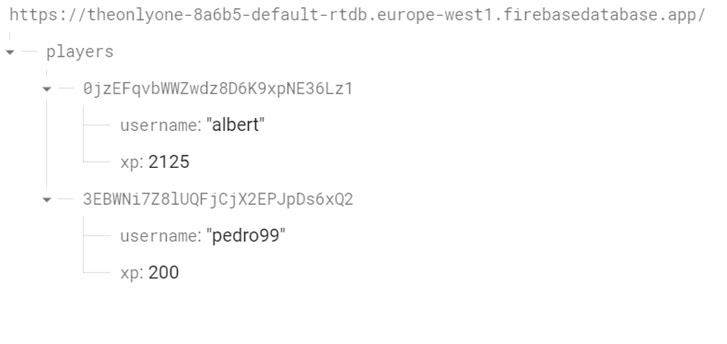
\includegraphics[scale=0.45]{img/DatabaseNoSQL.jpg}
	\caption{Datos almacenados en formato JSON}
	\label{fig:EstructuraJSON}
    \end{figure}
Para que el acceso de lectura y escritura de la base de datos esté restringido y por tanto protegido, todos los usuarios de la aplicación deben identificarse.

Gracias a \textbf{\textit{Firebase Authentication}}, se pueden definir de manera sencilla qué método de autenticación tendrá la aplicación. Para este proyecto se ha utilizado un procedimiento mediante el cual cada usuario debe proporcionar un correo y una contraseña para poder acceder a su cuenta.

Además, para garantizar la seguridad en la base de datos, Firebase proporciona reglas de seguridad para determinar quién puede acceder y/o modificar qué datos, y cómo se estructuran los datos.
Las reglas definidas en la aplicación son:
\begin{enumerate}
    \item Solamente los usuarios autenticados pueden leer los datos de los demás usuarios.
    \item Un usuario solamente puede escribir sus propios datos y no los de los demás usuarios.
\end{enumerate}
Cuando un usuario nuevo se registra en la aplicación, la clase FireBaseManager crea una nueva entrada en la base de datos asociada a al jugador, junto a un identificador único asignado por el propio gestor, el nombre de usuario que eligió al registrarse y la experiencia (xp) inicial vacía (0). 

Cuando este jugador inicie sesión, la base de datos ya lo tendrá localizado, permitiéndole ir al menú principal, donde verá su nombre de usuario y su experiencia actual. 
Además de sus propios datos, también podrá ver los datos de los jugadores con más experiencia del juego accediendo al apartado ``clasificación'', donde se muestran sus nombres de usuario y sus respectivas experiencias. Al momento de pulsar dicho botón, la clase \textit{GetUsersData} hace una petición de consulta a la base de datos para recuperar los datos de los mejores jugadores del videojuego, en orden de mayor a menor. Entonces, el videojuego crea una fila visual para cada jugador con su información para ser mostrada en la clasificación.

Para que el usuario pueda aumentar su experiencia, deberá completar partidas, y dependiendo de su desempeño en ellas, ganará más o menos experiencia. Al terminar una partida, la clase \textit{GameManager} enviará una petición de escritura a la base de datos para modificar el atributo correspondiente a la experiencia del usuario, sumándole la ganada en dicha partida.
Concretamente, se utiliza la función \textbf{\textit{SetValueAsync()}} para escribir y actualizar algún atributo específico, y \textbf{\textit{GetValueAsync()}} para obtener una instantánea estática del contenido de la ruta especificada que contendrá todos los datos pedidos, a partir de la cual se extraen los datos deseados.
El flujo de datos entre la aplicación y la base de datos se puede visualizar de manera esquematizada en la figura \ref{fig:EsquemaBBDD}:
\begin{figure}[h]
	\centering
	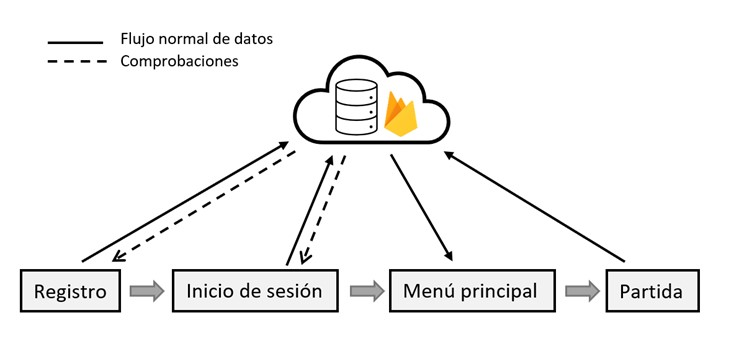
\includegraphics[scale=0.45]{img/DataFlowDiagram.jpg}
	\caption{Esquema del flujo de datos con la base de datos}
	\label{fig:EsquemaBBDD}
    \end{figure}
\subsection{Managers}
A la hora de definir la jerarquía de clases del proyecto, existen algunas clases que se definen como Managers o Gestores de las demás. Estas actúan como controladores de diferentes secciones del videojuego, centralizando varios elementos y asegurándose de que todo funciona como se espera. En este proyecto, existen algunas clases a destacar de este estilo, que suelen ser referenciadas de manera recurrente por el resto de clases.

La clase \textbf{\textit{SceneDirector}} (ver figura \ref{fig:SceneDirector}) es la responsable del manejo de escenas de la aplicación. Cada vez que se desea cambiar de escena se debe llamar a esta clase, y en concreto a su método \textit{LoadScene(escena)}, que internamente hará lo necesario para cargar la escena objetivo de forma consistente, mostrando una pantalla de carga durante el proceso. También será la clase llamada cuando se quiera cerrar la aplicación, con el método \textit{QuitGame()}.

\begin{figure}[h]
	\centering
	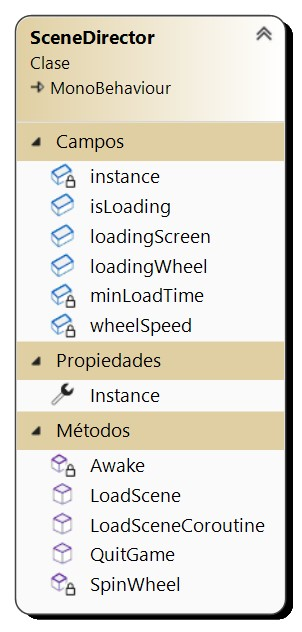
\includegraphics[scale=0.45]{img/SceneDirector.jpg}
	\caption{Clase \textit{SceneDirector}}
	\label{fig:SceneDirector}
    \end{figure}

\textbf{\textit{AudioManager}} (ver figura \ref{fig:AudioManager}) es la clase encargada de gestionar gran parte de los sonidos generales del videojuego, como los relacionados con la música, los botones de las interfaces, y todos los relativos al jugador, como los efectos sonoros de curarse y recibir daño.
\begin{figure}[h]
	\centering
	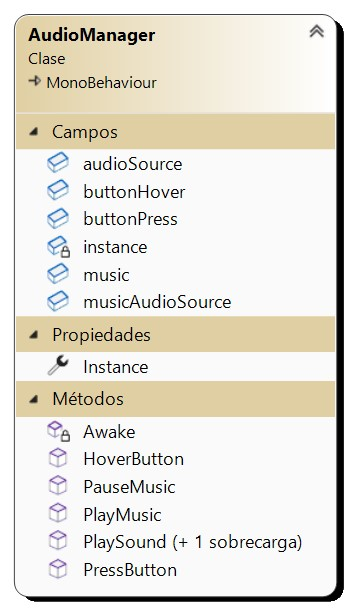
\includegraphics[scale=0.45]{img/AudioManager.jpg}
	\caption{Clase \textit{AudioManager}}
	\label{fig:AudioManager}
    \end{figure}
Ambas clases implementan el patrón de diseño Singleton \cite{wiki:Singleton}, un patrón de diseño creacional que permite asegurar que una clase tiene una única instancia, al tiempo que proporciona un punto de acceso global a dicha instancia. Además, se marcan con el método \textit{DontDestroyOnLoad()} \cite{doc:DontDestroyOnLoad} para que los gameobjects que las contienen no se destruyan al cambiar de escena y así poder acceder a ellos y, por tanto, a las clases desde cualquier escena. Esto es importante para mantener la consistencia de datos a través de toda la aplicación y evitar errores asociados a la duplicidad o ambigüedad de elementos.\\
Por ejemplo, si el objeto que contiene a la clase \textit{AudioManager} se destruyese al cambiar de una escena a otra, la música que pueda estar sonando se pararía y volvería a comenzar de nuevo. Esto se evita con las técnicas descritas, pudiendo tener un hilo de música continuo en toda la aplicación.

La clase \textbf{\textit{ButtonsManager}} (ver figura \ref{fig:ButtonsManager}) tiene como objetivo centralizar y gestionar el comportamiento de todos los botones presentes en la aplicación, para, de esta forma, tenerlos más organizados y que puedan ser modificados y administrados más fácilmente. En este caso no se requiere mantener una única referencia de esta clase en toda la aplicación, ya que cada escena la utilizará unos atributos distintos en función de la escena actual, a diferencia de las dos clases anteriores, cuyos atributos son consistentes en todo el sistema.
\begin{figure}[h]
	\centering
	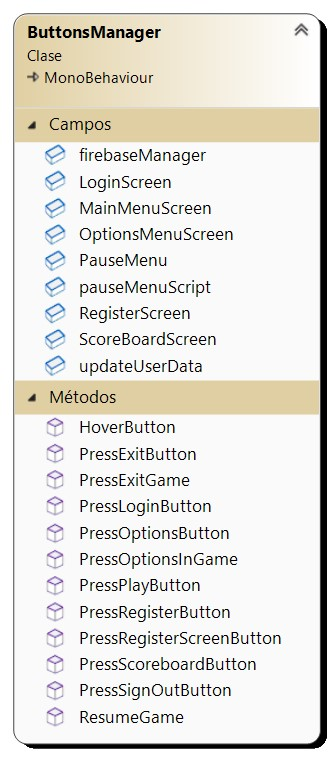
\includegraphics[scale=0.45]{img/ButtonsManager.jpg}
	\caption{Clase \textit{ButtonsManager}}
	\label{fig:ButtonsManager}
    \end{figure}
Además de la autenticación, \textbf{\textit{FirebaseManager()}} (ver figura \ref{fig:FirebaseManager})gestiona todos los aspectos relacionados con la base de datos del videojuego, incluyendo los datos de los usuarios y la consistencia de los mimos. Contiene ciertos atributos estáticos para que sean accesibles en cualquier lugar a nivel de clase, como ``Auth'' (autenticación), ``User''(usuario activo) y ``DBReference'' (base de datos).
\begin{figure}[h]
	\centering
	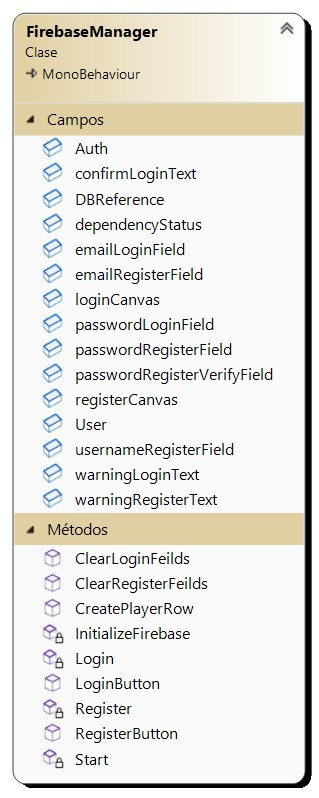
\includegraphics[scale=0.45]{img/FirebaseManager.jpg}
	\caption{Clase \textit{FirebaseManager}}
	\label{fig:FirebaseManager}
    \end{figure}
Por último, una de las clases más importantes en la jerarquía es la clase \textbf{\textit{GameManager}} (ver figura \ref{fig:GameManager}), responsable de que todos los elementos, una vez iniciada la partida, funcionen e interactúen entre ellos adecuadamente para garantizar la correcta ejecución del juego.

Entre sus funciones destacan:
\begin{itemize}
    \item Llevar la cuenta del número de entidades (jugador y enemigos) que siguen vivos, un elemento muy relevante dentro del género battle royale
    \item Actualizar algunos elementos visuales como los enemigos que quedan, los que ha eliminado el jugador o la munición del arma activa, si la hubiere.
    \item Detectar si la partida termina
    \item Determinar el puesto en que queda el jugador al terminar la partida (y si gana o no)
    \item Calcular la experiencia ganada por el jugador durante la partida
    \item Actualizar la experiencia del jugador en la base de datos
    \item Generar las etiquetas flotantes de los objetos de la partida que lo requieran
    \item Mostrar las pantallas de victoria, derrota o estadísticas con la respectiva información
    \item Una de sus funciones principales consiste en convertirse en un lugar centralizado donde definir varios elementos y datos que se utilizarán durante la partida:
    \begin{itemize}
    \item Tipos de armas que pueden existir
    \item Rarezas disponibles de cada arma
    \item Tipos de granadas que pueden existir
    \item Tipos de enemigos que pueden existir
    \item Tipos de packs de ayuda que pueden existir
    \item Rarezas disponibles de cada pack de ayuda
    \item Objetos que se pueden encontrar en las cajas de suministros o que suelten los enemigos al morir
    \end{itemize}
    \item También se definen algunos valores relevantes para la partida, como el radio inicial de la zona segura o cuánta experiencia gana el jugador por cada enemigo eliminado, por completar la partida o por ganarla.
\end{itemize}
\begin{figure}[h]
	\centering
	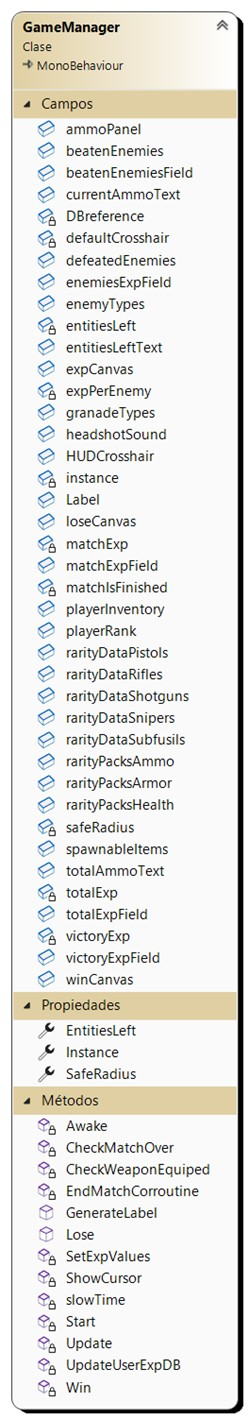
\includegraphics[scale=0.45]{img/GameManager.jpg}
	\caption{Clase \textit{GameManager}}
	\label{fig:GameManager}
    \end{figure}
Otras dos clases a destacar que se encargan de gestionar datos de otras clases son \textbf{\textit{PlayerController}} y \textbf{\textit{EnemyController}} (ver figura \ref{fig:ControladoresJugadorYEnemigo}). Cada una de ellas controla el comportamiento general del jugador y de los enemigos, respectivamente, junto a otras clases más específicas.
\begin{figure}[h]
	\centering
	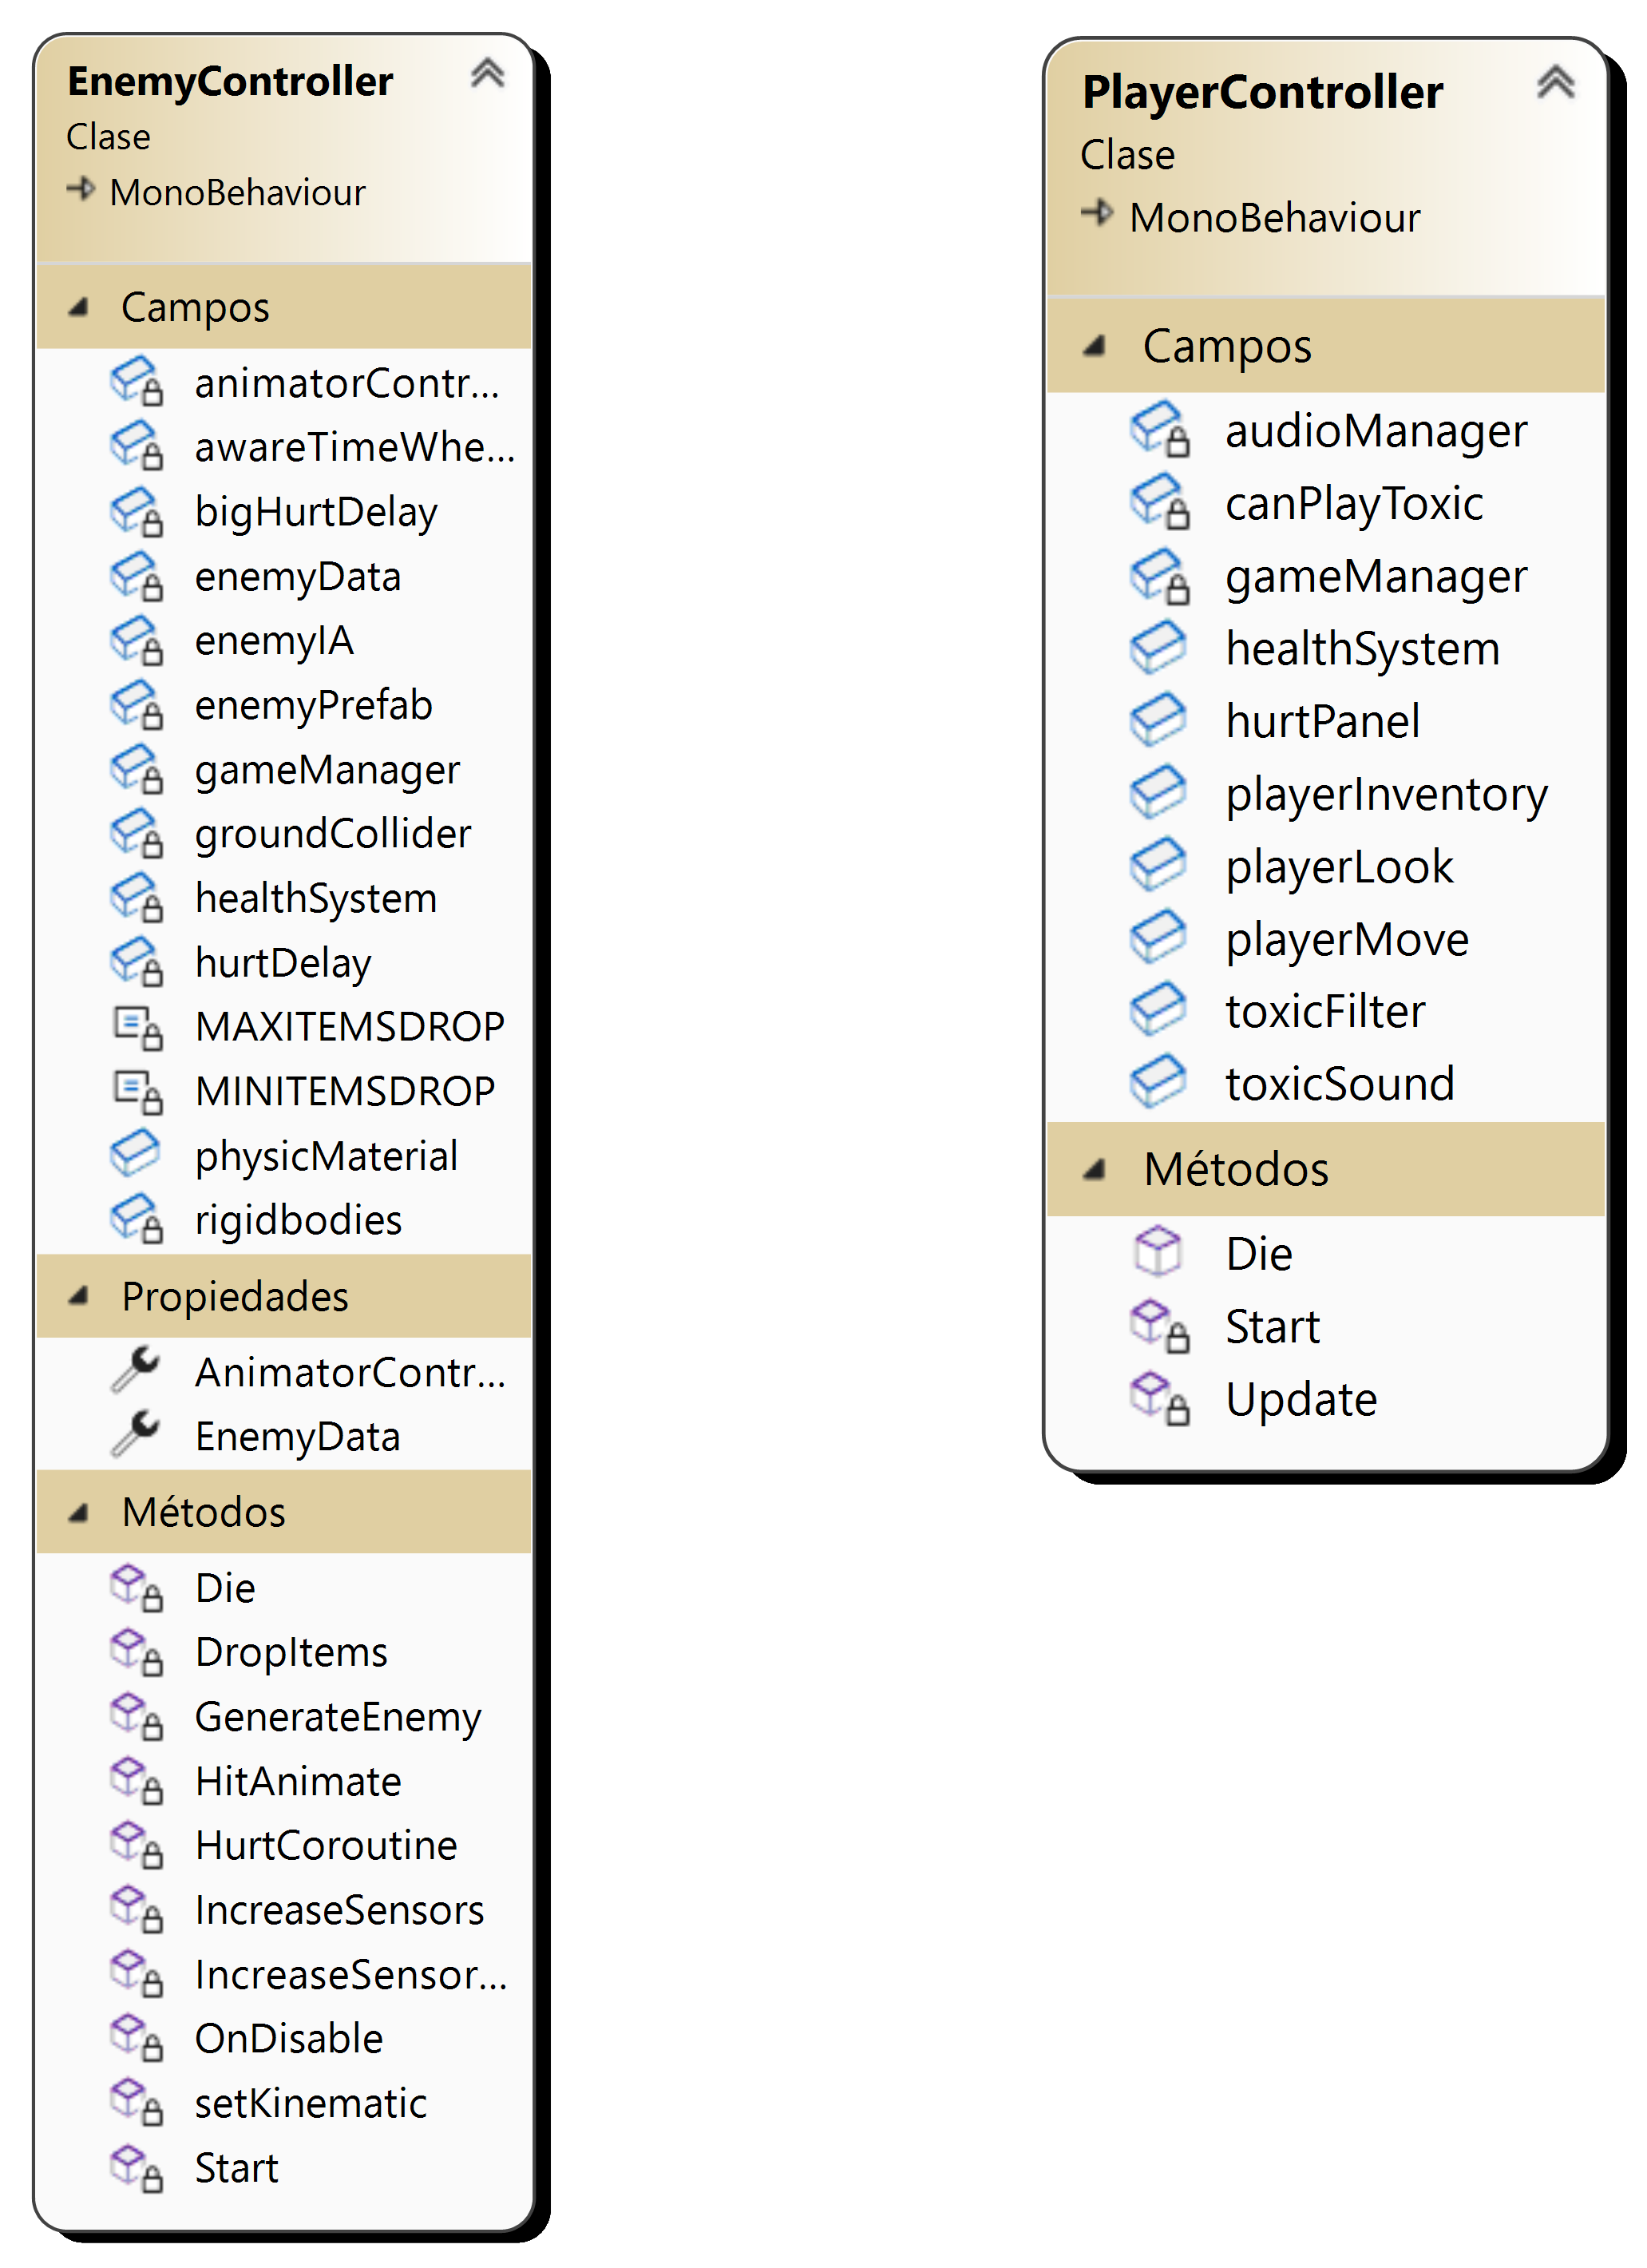
\includegraphics[scale=0.45]{img/PlayerAndEnemyControllers.png}
	\caption{Clases controladoras del jugador y los enemigos}
	\label{fig:ControladoresJugadorYEnemigo}
    \end{figure}
\textit{EnemyController}, por ejemplo, asigna los atributos y valores que tendrá el enemigo cuando se genere en la escena, monitoriza aspectos como la vida, la inteligencia, las animaciones, la interacción con el entorno, las colisiones, y gestiona sus diferentes componentes, desactivándolos cuando este muere, entre otros aspectos.

\subsection{ScriptableObjects}
Un aspecto muy relevante en el diseño de los datos del sistema ha sido el uso de los llamados ScriptableObjects. 

Los \textbf{\textit{ScriptableObjects}} son contenedores de datos con la peculiaridad de que son independientes de las instancias de clase, es decir, que a diferencia de las clases que heredan de \textit{MonoBehaviour}, los scriptableObjects no se pueden asociar a un GameObject como un componente más, sino que se guardan como un asset “estático” del proyecto, manteniéndose persistentes entre sesiones y accesibles mediante referencias.

Los datos almacenados en un scriptableObject son inmutables en el momento de ejecución, una vez la aplicación ha sido compilada, por lo que este tipo de contenedores son ideales para almacenar información que no cambiará durante la ejecución del programa y que vaya a ser consultada por varios objetos en la escena.

Por ejemplo, si se almacenan todos los datos de un gameobject en un script que herede de Monobehaviour y este se añade al gameobject como un componente, creando así un prefab, cada vez que se instancie dicho prefab, se cargará en memoria una copia completa de los datos por cada prefab que exista, lo que puede afectar gravemente al uso de memoria y, por tanto, al rendimiento de la aplicación.

Para solucionar esto, si hay datos del prefab que no son propios de cada instancia, sino comunes a todas ellas porque no van a cambiar durante la ejecución del programa, una mejor aproximación sería almacenar esta información como un scriptableObject, y después incluir en el script una referencia a este scriptableObject.

La razón de esto es que cuando en un script normal se referencia a un scriptableObject, solamente almacenan esa referencia que apunta al scriptableObject y no una copia completa de los datos que contiene. De esta forma se obtiene un mejor diseño de los datos, con un uso de memoria más optimizado y en general un mejor rendimiento de la aplicación.

En el proyecto se han utilizado 4 clases a modo de plantilla, que heredan de ScriptableObject para crear todos los scriptableObjects que se usan en el juego. Estas clases son \textbf{\textit{GranadeBlueprint}}, \textbf{\textit{WeaponBlueprint}}, \textbf{\textit{EnemyBlueprint}} e \textbf{\textit{ItemRarityBlueprint}} asociadas a los diferentes enemigos, granadas, rarezas de objetos y armas, respectivamente (ver figura \ref{fig:ScriptableObjects}).

\begin{figure}[h]
	\centering
	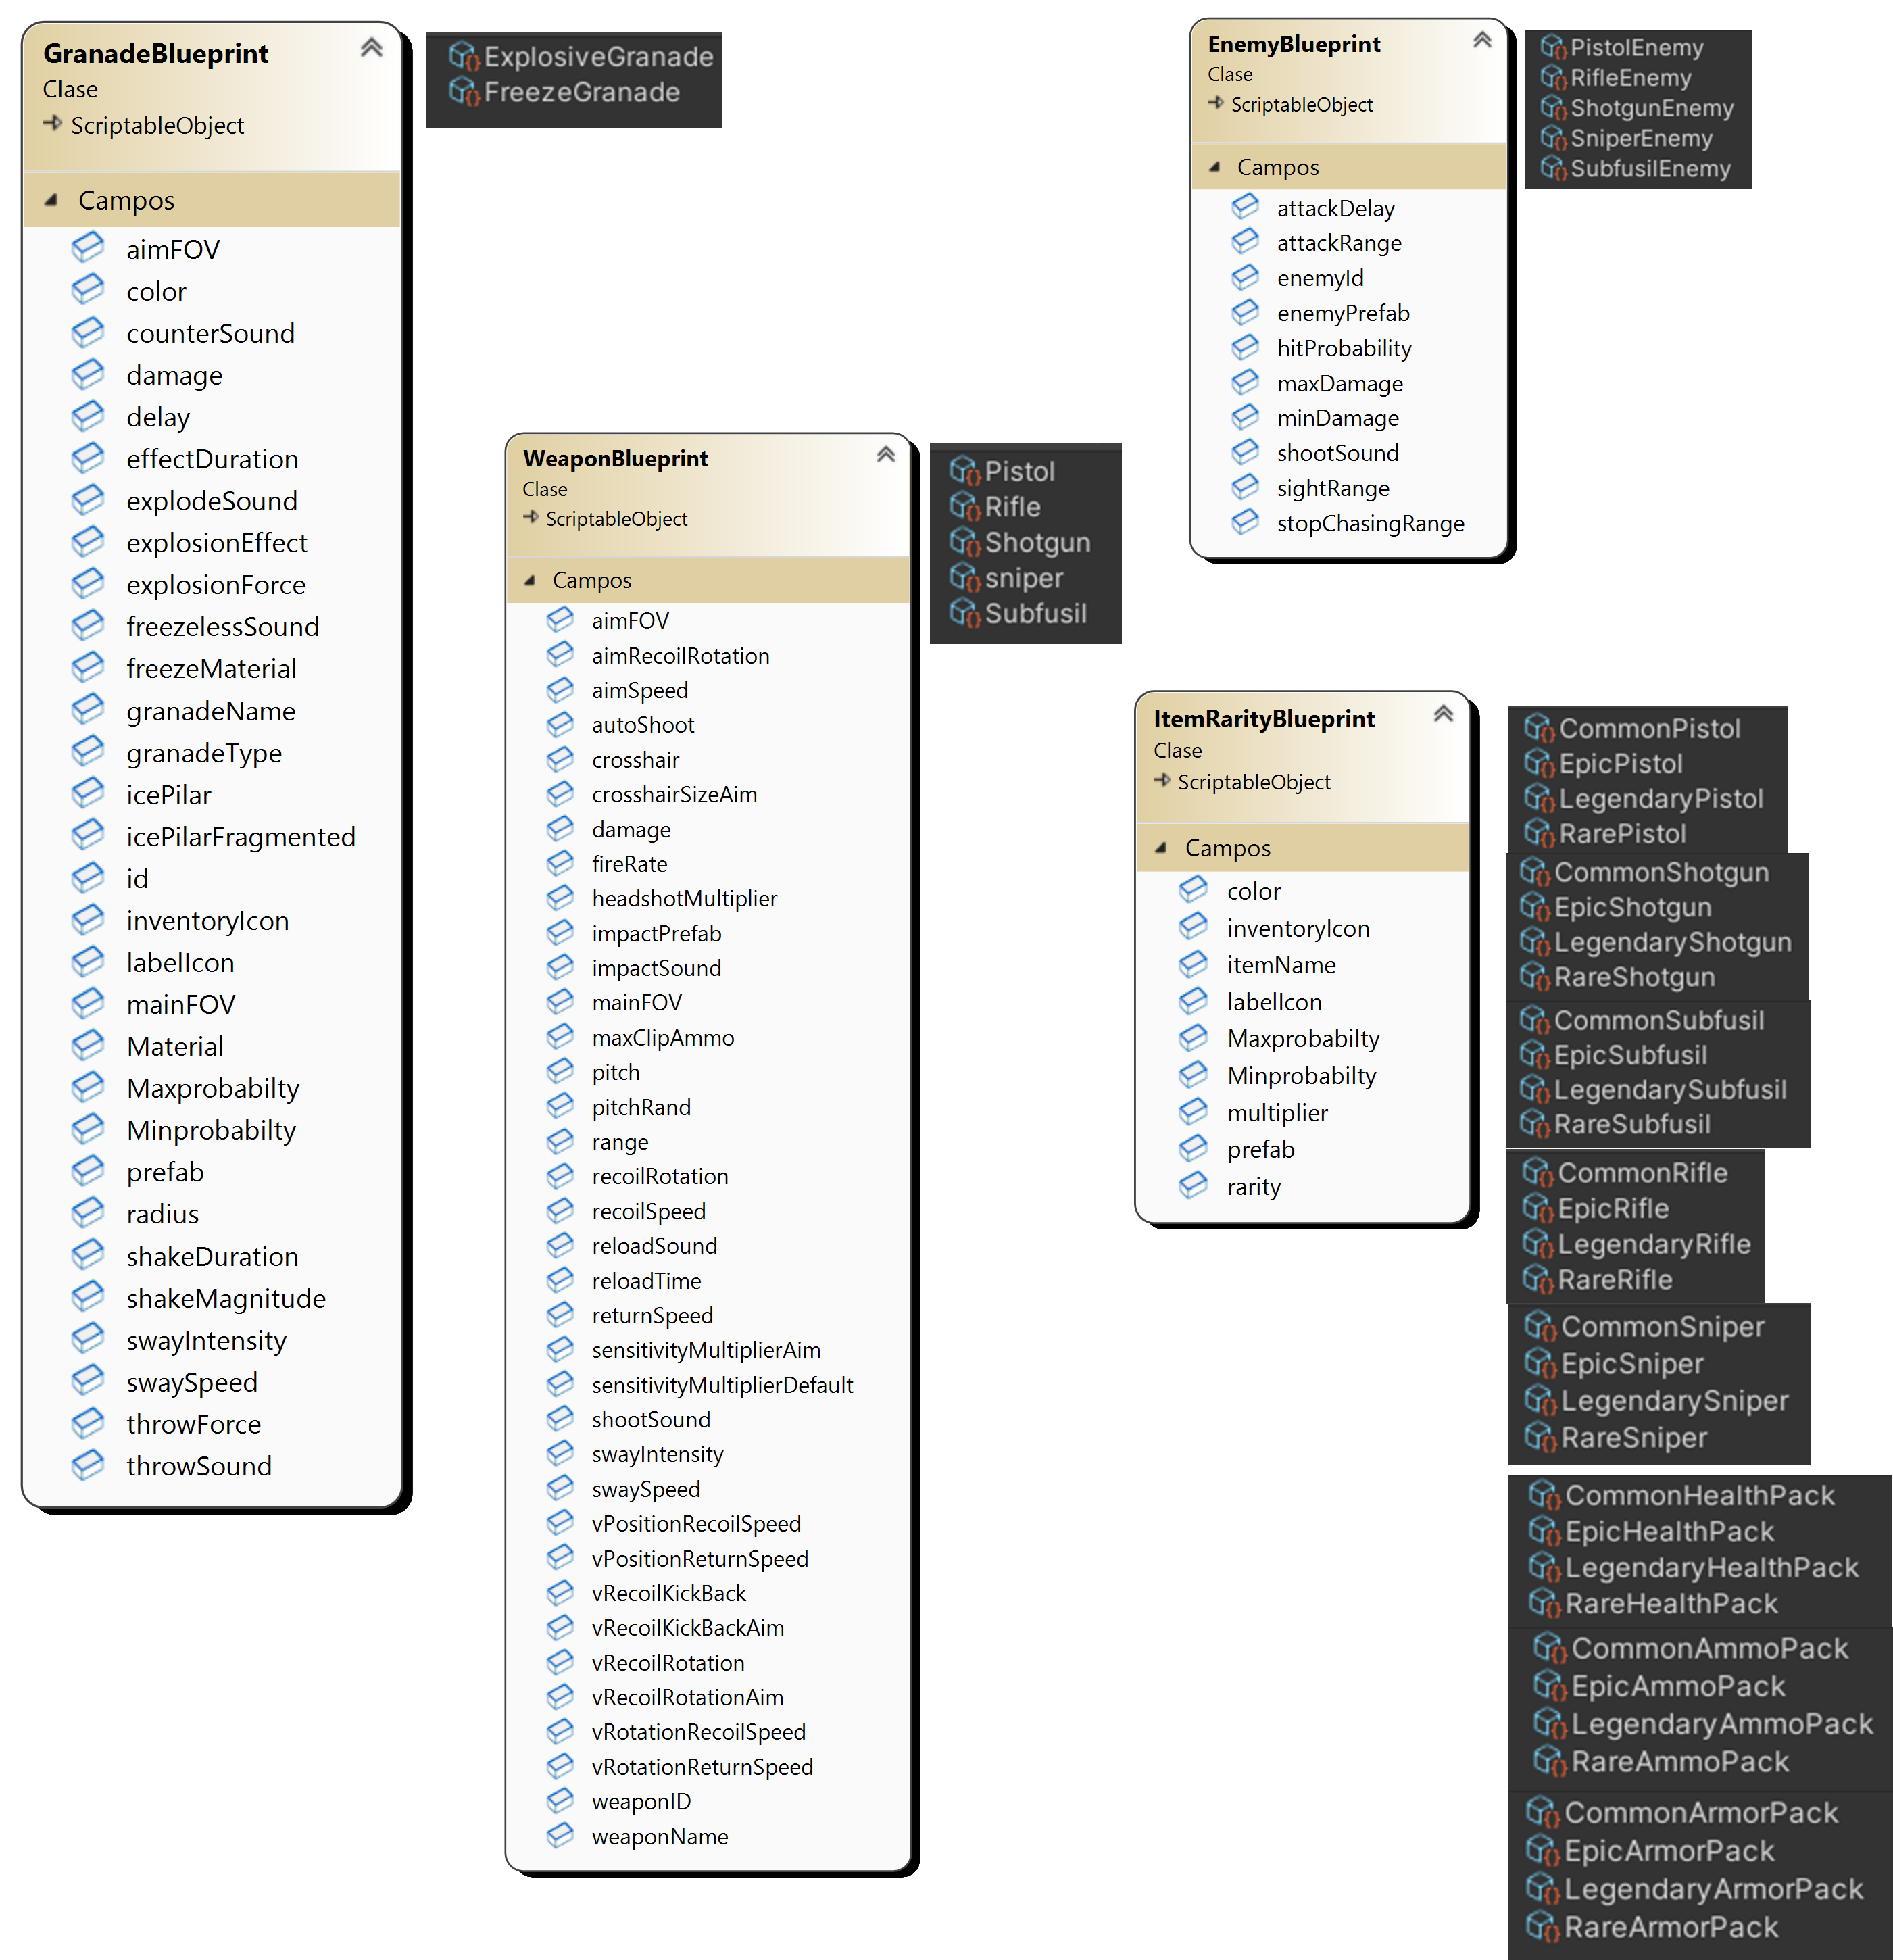
\includegraphics[scale=0.45]{img/Blueprints.png}
	\caption{Clases que heredan de ScriptableObject}
	\label{fig:ScriptableObjects}
    \end{figure}
    
Con el objetivo de ejemplificar el uso de estas estructuras de datos en el propio proyecto, se resumirá el flujo de trabajo con ScriptableObjects para la creación de los distintos tipos de enemigos que hay en el videojuego.

\subsubsection{Diseño de los enemigos}
Antes de crear un scriptableObject como tal se debe crear una clase que herede de la clase ScriptableObject, la cual actuará a modo de plantilla, con los datos que se desean almacenar. A partir de esta se crearán los diferentes scriptableObjects, cada uno con sus valores propios, que podrán ser usados más tarde en otros scripts.

La clase que actúa como plantilla de datos para los enemigos es \textit{EnemyBlueprint}, que, como se ha mencionado, deriva de la clase \textit{ScriptableObject}.

En este contenedor se deben definir los datos que se van a almacenar que, como se ha mencionado previamente, deben ser característicos del objeto (en este caso del enemigo) al que hagan referencia y no pueden cambiar una vez se inicie la aplicación.

Los datos que se mantendrán invariables, en este caso, son aspectos como el modelo 3D, el mínimo y máximo daño que puede hacer, el tiempo que hay entre sus ataques, la probabilidad de que acierte a su objetivo cuando dispare o su rango de vista y ataque. 

Sin embargo, otros atributos que sí irán cambiando a lo largo de la partida, como sus puntos de vida o su estado, deben almacenarse fuera de este contenedor para poder modificarse en tiempo de ejecución.

Una vez definidos los datos, se crean, a partir de esta plantilla, 5 assets desde el editor, todos con los mismos campos, que deben rellenarse con distintos valores en función de los tipos de enemigo que se quieran generar y sus características (ver figura \ref{fig:ScriptableObjectEnemigo}).
\begin{figure}[h]
	\centering
	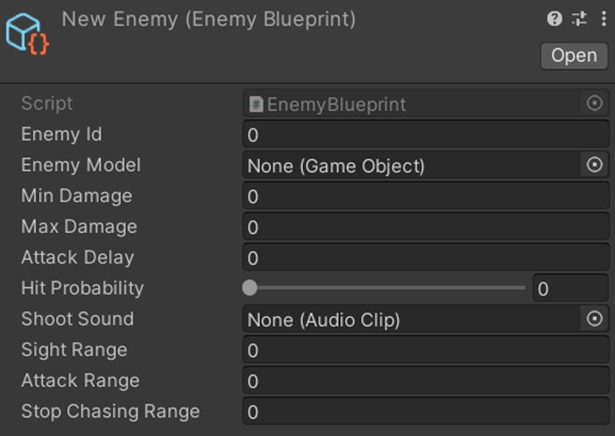
\includegraphics[scale=0.45]{img/EnemyScriptableObject.jpg}
	\caption{ScriptableObject de los enemigos}
	\label{fig:ScriptableObjectEnemigo}
    \end{figure}
Tras almacenar todos los valores estáticos de los posibles enemigos en diferentes scriptableObjects, se crea la ya mencionada clase \textit{EnemyController}, esta vez como típicamente se crea un script en el juego, heredando de \textit{MonoBehaviour}, en la que se incluye una referencia del tipo \textit{EnemyBlueprint}. Este atributo podrá referenciar a uno de los scriptableObjects del proyecto, al igual que el tipo int puede tomar los valores 1, 24 o 829.

De esta forma, se podrían crear \textbf{5 prefabs diferentes}, uno por cada tipo de enemigo en el juego y que cada uno contuviese una referencia al scriptableobject correspondiente.

En este caso, no se conocerá de antemano el tipo de enemigo que va a representar un prefab \textit{enemy} al momento de arrastrarlo a la escena, sino que será el \textit{GameManager} (es allí donde se tiene un array de referencias a todos los scriptableobjects) quien escoja aleatoriamente un scriptableObject de un tipo de enemigo, y después el \textit{EnemyController} ligado al prefab, construirá el enemigo escogido con los datos del scriptableobject elegido.   

Utilizando este diseño en los datos, se consigue tener un único prefab para generar todos los enemigos del juego (ver figura \ref{fig:PrefabEnemigos}).
\begin{figure}[h]
	\centering
	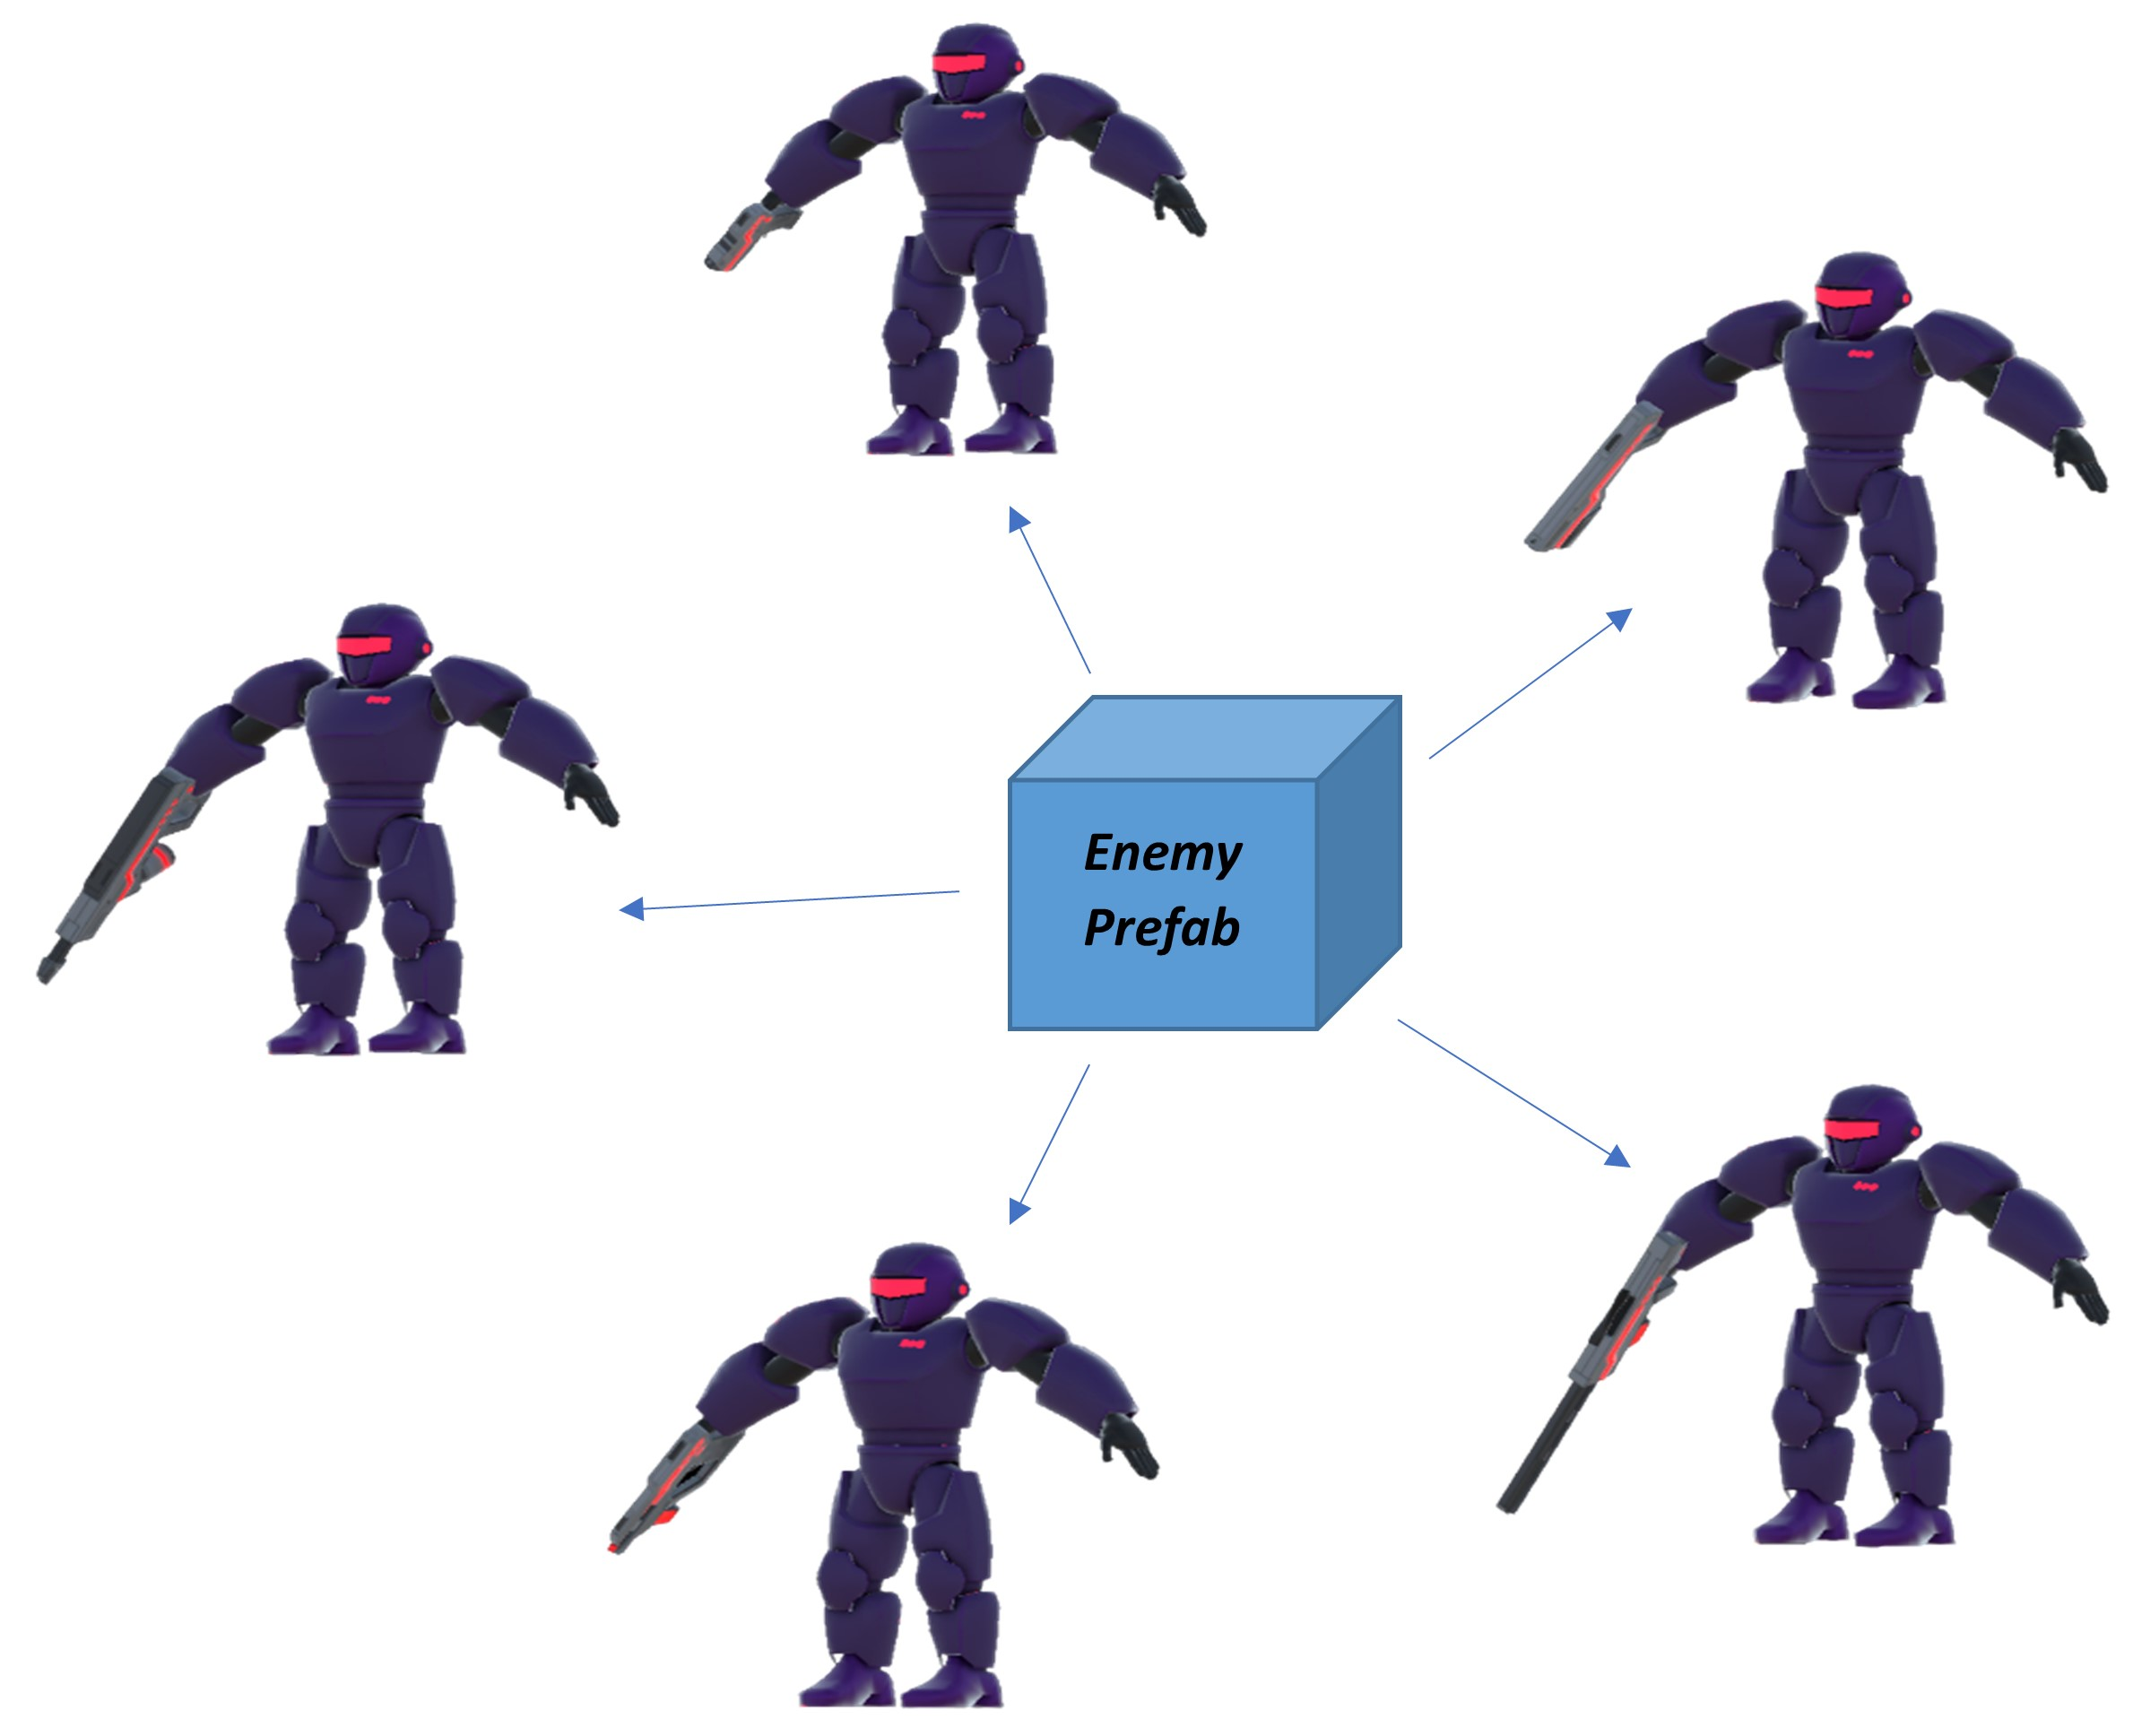
\includegraphics[scale=0.45]{img/EnemyPrefab.jpg}
	\caption{Único prefab para todos los enemigos}
	\label{fig:PrefabEnemigos}
    \end{figure}
Además, gracias a los scriptableObjects, cada vez que se instancie un enemigo de un tipo, los datos comunes a ese tipo no se duplicarán sino que accederán todos al mismo contenedor de datos (ver figura \ref{fig:PistolEnemyScriptableObject}), algo que mejora en gran medida la eficiencia general del programa y más, teniendo en cuenta la gran cantidad de enemigos que puede haber simultáneamente en este género de videojuegos (50-100).
\begin{figure}[h]
	\centering
	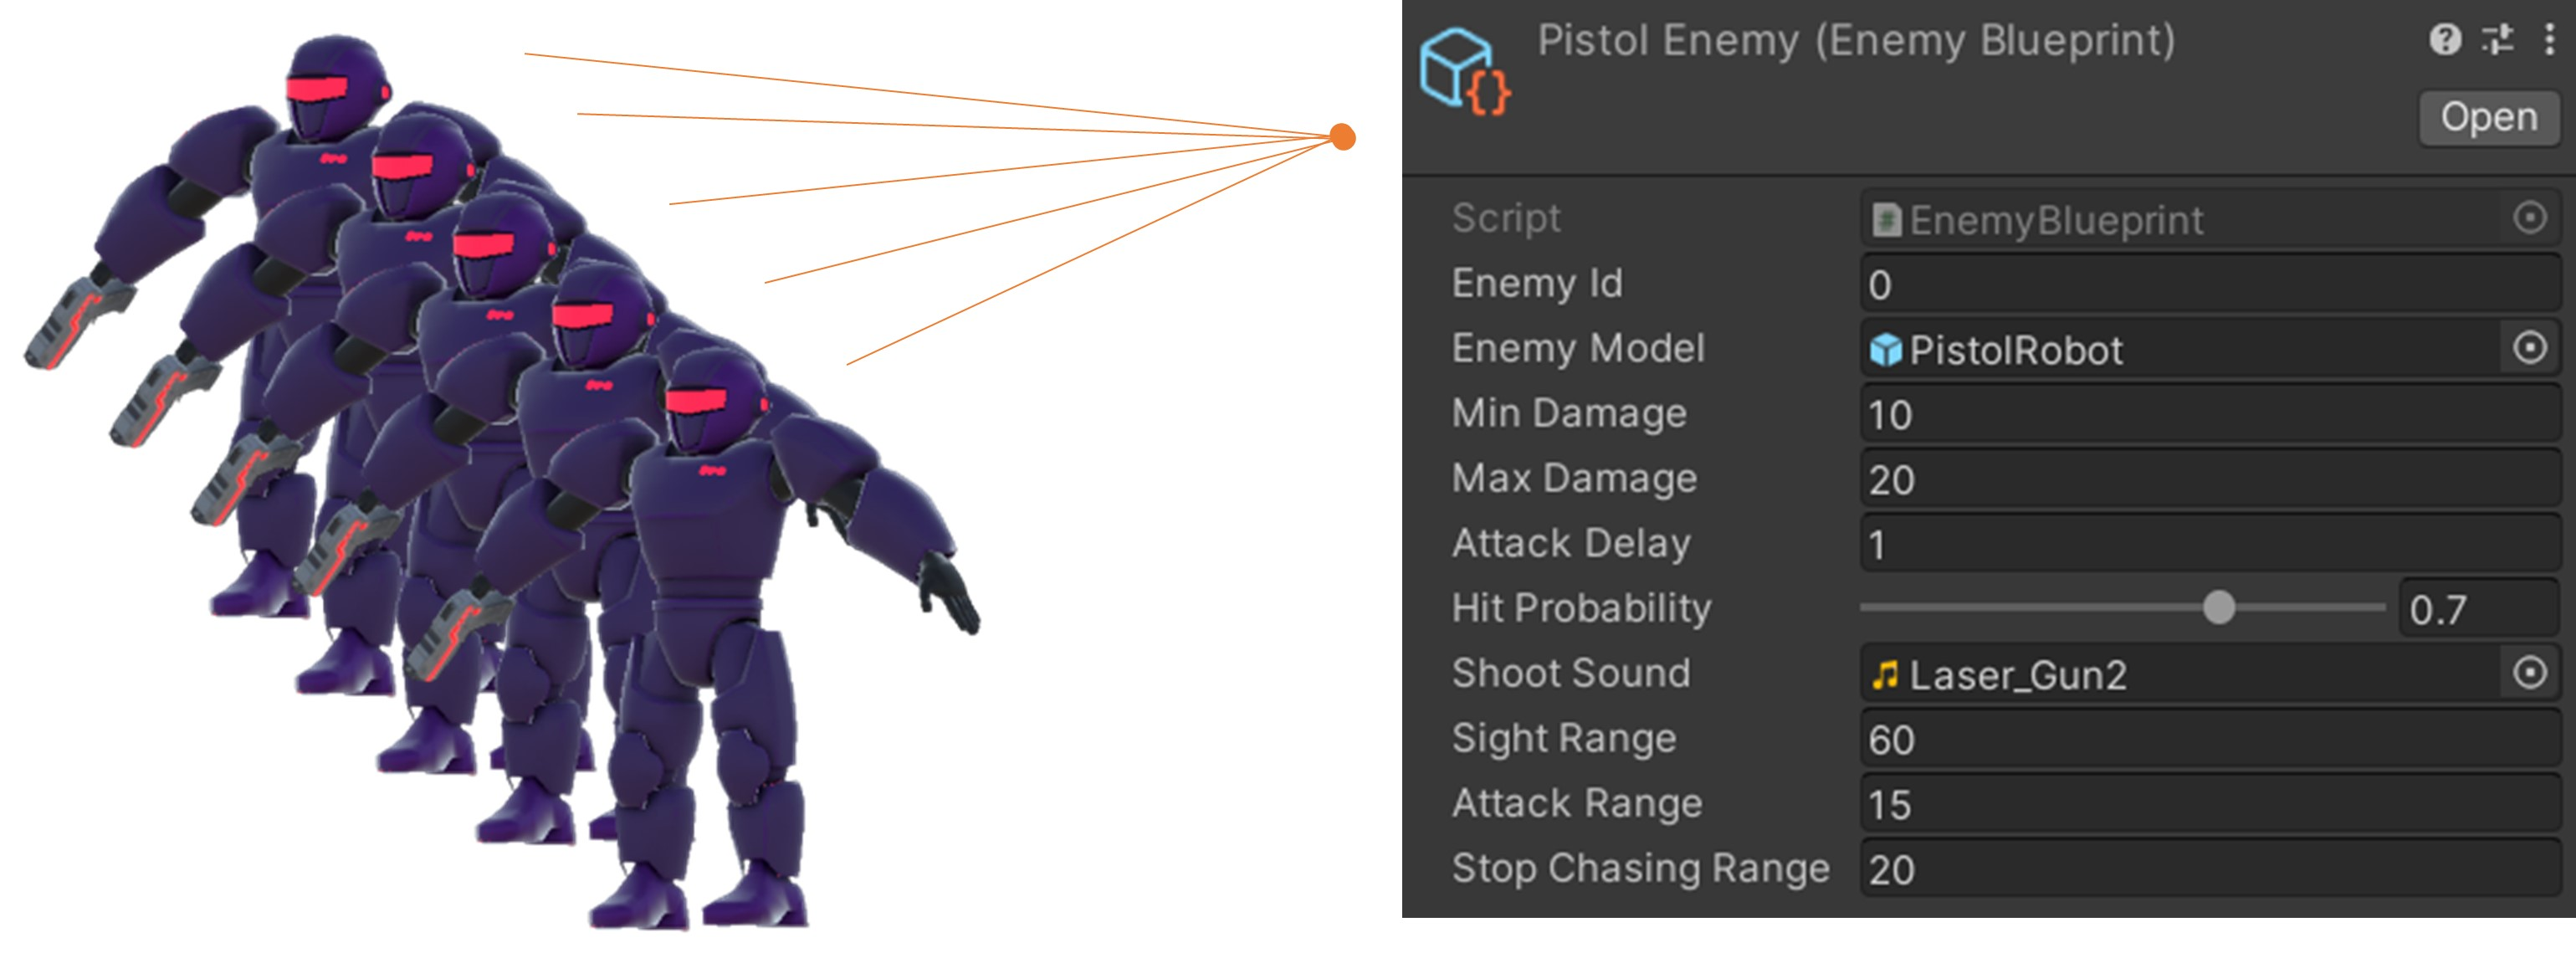
\includegraphics[scale=0.45]{img/PistolEnemyScriptableObject.jpg}
	\caption{Varios objetos acceden al mismo contenedor de datos}
	\label{fig:PistolEnemyScriptableObject}
    \end{figure}
Es más, atendiendo al objetivo de escalabilidad y \textbf{extensibilidad}, si se desea añadir un nuevo tipo de enemigo al juego, simplemente se tendría que crear un nuevo scriptableObject a partir de la plantilla, rellenar sus campos y añadir ese objeto al array de referencias de enemigos en la clase GameManager, facilitando así el proceso de incluir nuevo contenido al videojuego.

De esta forma, al arrastrar el Prefab del enemigo a la escena, el nuevo tipo de enemigo ya sería candidato para generarse por el Prefab cuando se inicie el programa.

En los diagramas de clases mostrados en este apartado se puede observar que no hay clases que hereden unas de otras, y es que los scriptableobjects sustituyen en gran medida a clases genéricas, ya que son contenedores con atributos comunes, que bien podrían representar este tipo de clases si no existiesen los scriptableObjects.

\subsection{Events} \label{Events}
Otro elemento clave en el diseño de los datos de la aplicación para que la información de las clases se comunique entre sí son los llamados eventos (\textit{events}) de Unity.

Un \textbf{\textit{event}} no es más que una forma de anunciar que algo concreto ha pasado en algún script, para quien quiera escucharlo, lo sepa.

En un evento hay dos tipos de participantes. Quien envía el evento se llama \textbf{\textit{publisher}}, y quienes lo escuchan se denominan \textbf{\textit{subscribers}} o suscriptores. Cuando algo concreto ocurre, el \textit{Publisher} anuncia el evento, y los subscribers son notificados de que el evento ha ocurrido.

La clave de este diseño es que el \textit{Publisher} no sabe quiénes son sus suscriptores, si los tuviera, lo que permite obtener modularidad en el traspaso de datos, teniendo, por un lado, el código principal en el Publisher y, por otro lado, en los subscribers, funcionalidades adicionales no esenciales a la acción del Publisher.

En el videojuego se han utilizado los eventos principalmente para mantener la \textbf{lógica separada de lo visual} en elementos como el inventario o el sistema de salud. De esta manera, la lógica puede seguir funcionando aún sin los elementos visuales, ya que no contendrá ningún tipo de referencia hacia ellos.\\
También permite reutilizar más fácilmente el código del Publisher y añadir nuevos elementos visuales asociados a él más fácilmente, lo que responde a los objetivos de usabilidad, extensibilidad y eficiencia.

A continuación se describe el diseño del sistema de salud y cómo utiliza los \textit{events}.

La clase \textbf{\textit{HealthSystem}} contiene toda la lógica del sistema de salud tanto del jugador como de los enemigos. Será por tanto quien publique los eventos. Se definen 4 eventos diferentes (ver figura \ref{fig:EventosHealthSystem}), asociados a los principales sucesos que pueden ocurrir en en esta clase: Recibir daño, recuperar salud, recuperar armadura, y morir.

\begin{figure}[h]
	\centering
	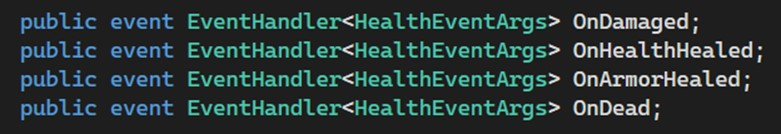
\includegraphics[scale=0.45]{img/HealthEventArgs.jpg}
	\caption{Definición de eventos en la clase ``HealthSystem''}
	\label{fig:EventosHealthSystem}
    \end{figure}
    
Cabe destacar que cuando se anuncia un evento, este puede contener algunos \textbf{argumentos} que se enviarán junto al evento para que los subscribers puedan trabajar con ellos. El tipo de argumentos que se pueden usar se debe definir en clases especiales que hereden de la clase \textit{EventArgs}.

En este ejemplo, los eventos de la clase \textit{HealthSystem} podrán utilizar los argumentos definidos en la clase \textbf{\textit{HealthEventArgs}}.

De esta manera, cuando, por ejemplo, se llame al método \textbf{\textit{HealHealth(int amount)}} de la clase, además de la lógica pertinente que realice el método, como sumar \textit{amount} puntos de vida al atributo referente a la salud, \textbf{se disparará el evento \textit{OnHealthHealed}}, con \textit{amount} como argumento, anunciando que se ha recuperado cierta cantidad de salud en dicha instancia de la clase.\\
Las clases que estén suscritas a dicho evento serán notificadas y realizarán alguna acción al respecto.

La clase \textit{HealthSystemVisuals} es la encargada de actualizar todos los elementos visuales relacionados con la salud, como las barras de salud y armadura, los puntos de vida del jugador, los textos flotantes que aparecen al hacer daño a un enemigo o los efectos visuales y sonoros de daño, cura y armadura, entre otros.

Con el fin de poder actualizar dichos elementos, la clase está suscrita a los eventos que publica la clase \textit{HealthSystemVisuals} para así poder estar al tanto de sucesos que le interesan .

Para suscribirse a un evento y poder realizar una acción asociada a él se utiliza esta sencilla nomenclatura: \textbf{Evento += acción a realizar} (ver figura \ref{fig:SuscripcionesHealth}). De manera similar, si se desea que una clase deje de prestar atención a un evento, se utiliza la nomenclatura \textbf{Evento -= acción a realizar}.

\begin{figure}[h]
	\centering
	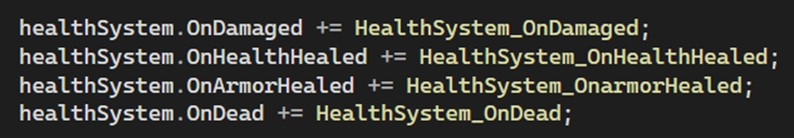
\includegraphics[scale=0.45]{img/HealthSystemVisuals.jpg}
	\caption{Suscripciones en la clase ``HealthSystemVisuals''}
	\label{fig:SuscripcionesHealth}
    \end{figure}
    
De esta manera, a modo de resumen, cuando se dispare el evento \textit{OnHealthHealed} en la instancia de \textit{HealthSystem} del jugador, la instancia correspondiente de \textit{HealthSystemVisuals} llamará a su método \textit{HealthSystem\_OnHealthHealed} para realizar acciones asociadas al evento, como actualizar la barra de salud del jugador y sus puntos de vida en la interfaz o reproducir el sonido y los efectos visuales asociados a la curación (ver figura \ref{fig:UMLHealth}).

\begin{figure}[h]
	\centering
	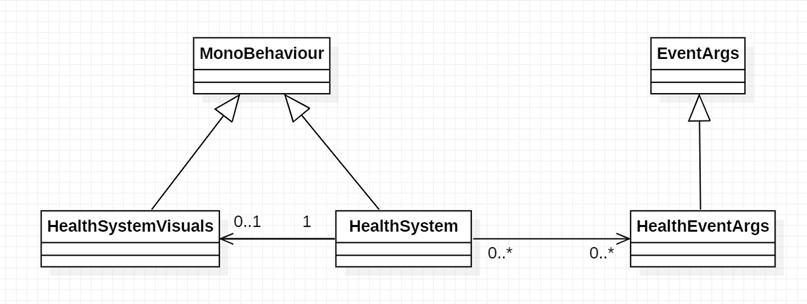
\includegraphics[scale=0.45]{img/UMLClassDiagram.jpg}
	\caption{Diagrama de clases UML del sistema de salud}
	\label{fig:UMLHealth}
    \end{figure}
    
Este método para separar los datos lógicos de los visuales se utiliza de manera similar en la clase \textbf{\textit{PlayerInventory}} (ver figuras \ref{fig:EventosInventario} y \ref{fig:SuscripcionesInventario}), que gestiona la parte lógica del inventario del jugador. En este caso, los eventos serán propios de un inventario, como añadir un objeto, tirar un objeto o cambiar el objeto activo, y la clase que escuche dichos eventos será \textbf{\textit{InventoryVisuals}}.

\begin{figure}[h]
	\centering
	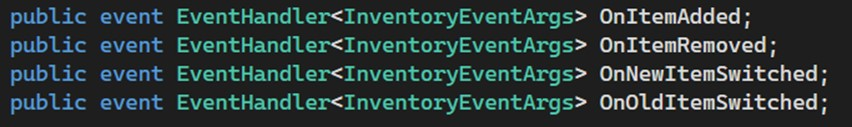
\includegraphics[scale=0.45]{img/InventoryEvents.jpg}
	\caption{Definición de eventos en la clase “PlayerInventory”}
	\label{fig:EventosInventario}
\end{figure}

\begin{figure}[h]
    \centering
    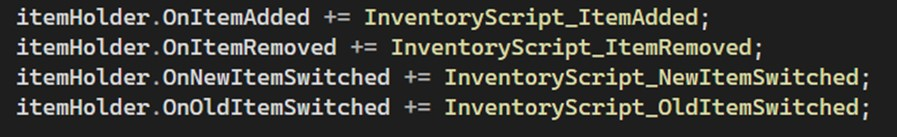
\includegraphics[scale=0.45]{img/InventorySubscribers.jpg}
    \caption{Suscripciones en la clase “InventoryVisuals”}
    \label{fig:SuscripcionesInventario}
\end{figure}
El uso de eventos en Unity es imprescindible para que los diferentes elementos se comuniquen entre sí de manera eficiente y se disponga de una estructura de clases adecuada con un código limpio y fácil de mantener (ver figura \ref{fig:EsquemaEventos}).

\begin{figure}[h]
    \centering
    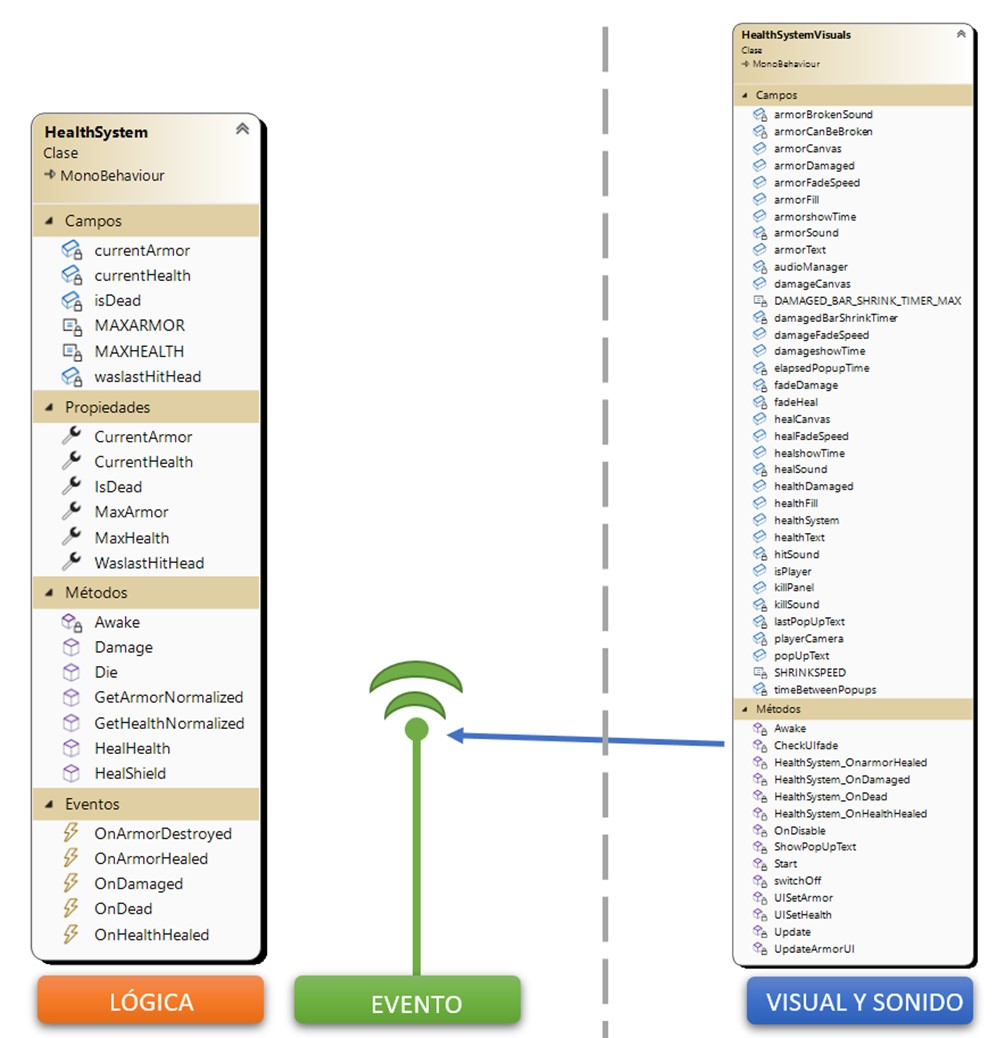
\includegraphics[scale=0.45]{img/EventsUnity.jpg}
    \caption{Esquema del funcionamiento de los eventos}
    \label{fig:EsquemaEventos}
\end{figure}

\subsection{Añadir arma nueva al juego}

Para ilustrar cómo se integran todos estos datos en el proyecto, se puede ver, por ejemplo, el proceso a través del cual se añade un nuevo tipo de arma al juego, ya que en él se incluyen varios de los elementos descritos anteriormente.

\begin{enumerate}
    \item \textbf{\textit{Crear recursos de diseño del arma}}
    Al querer incluir un arma nueva en el juego, se han de crear antes los elementos artísticos que van a componerla, como su modelo 3D, sus texturas o los efectos de sonido.
    
    Se ha utilizado el programa \textit{Audacity} \cite{wiki:Audacity} para crear y mezclar los sonidos de disparo y de recarga de todas las armas (ver figura \ref{fig:SonidosAudacity}).
    \begin{figure}[h]
    \centering
    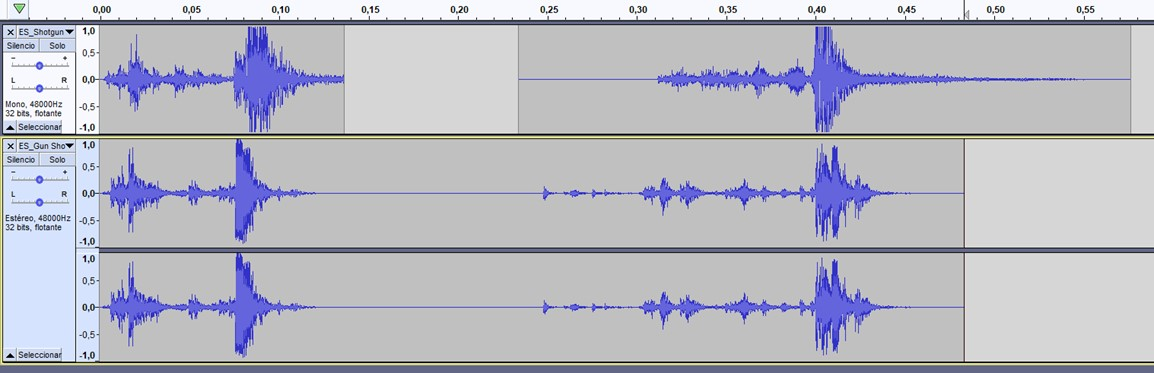
\includegraphics[scale=0.45]{img/AudacityScreenshot.jpg}
    \caption{Captura de Audacity con el sonido de Recarga de la escopeta}
    \label{fig:SonidosAudacity}
    \end{figure}
    Para los modelos 3D de las armas, se ha adquirido un pack de modelos en la tienda de Unity, en conjunción con el programa \textit{Blender} \cite{wiki:Blender} para crear partes nuevas o adaptar y modificar las existentes (por ejemplo para crear la mirilla telescópica del francotirador, que inicalmente no existía).\\
    En el caso concreto de la escopeta, se ha utilizado blender para crear y añadir la parte corredera de esta y diseñar su color y textura (ver figura \ref{fig:EscopetaBlender}).
    
    \begin{figure}[h]
    \centering
    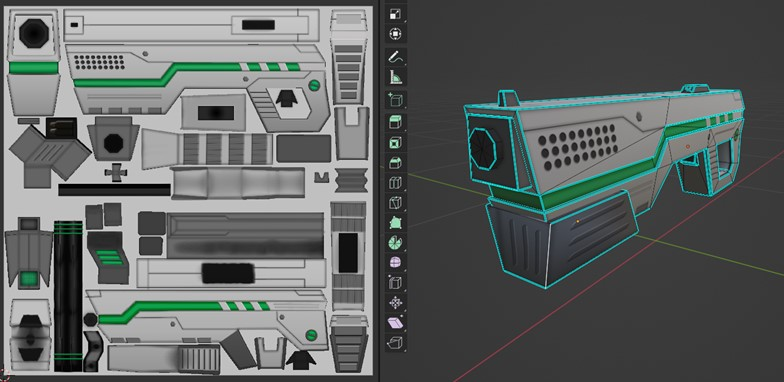
\includegraphics[scale=0.45]{img/ShotgunBlender.jpg}
    \caption{Modelo y textura princial de la escopeta}
    \label{fig:EscopetaBlender}
    \end{figure}
    
    \item \textbf{\textit{Importar los recursos a Unity}}
    Una vez se han creado los elementos necesarios, se deben importar a Unity en el formato adecuado para que se creen los assets correspondientes. Por ejemplo, los modelos de blender se pueden importan en formato .blend o .fbx, mientras que las pistas de audio se importan en formato .wav para que sean compatibles con el motor.
    Las texturas se suelen importar en formato .png.
    
    \item \textbf{\textit{Construir modelo y materiales}}
    Ya en Unity, se crea el material del arma con las texturas adecuadas y se añaden los atributos necesarios, como correcciones del color o diferentes mapas. Los mapas utilizados en el material del arma son la textura base, un mapa de normales o \textit{normal map}, que crea relieve de manera artificial en la textura, y un mapa de emisión o \textit{emission map}, que delimita las zonas de la textura que deben emitir luz. En este caso, la zona que debe brillar es la del color neón del arma (ver figura \ref{fig:TexturasEscopeta}).
    
    \begin{figure}[h]
    \centering
    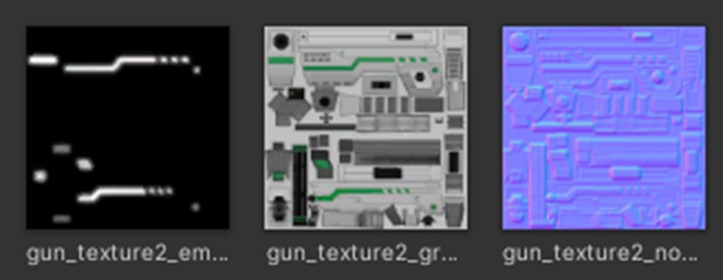
\includegraphics[scale=0.45]{img/ShotgunTexture.jpg}
    \caption{Mapas de texturas de la escopeta}
    \label{fig:TexturasEscopeta}
    \end{figure}
    
    Una vez creado el material, se adhiere al arma y después se acopla el arma al modelo de brazos del jugador para tener así el modelo completo que se verá una vez se sostenga el arma en primera persona (ver figura \ref{fig:Escopeta}).
    \\No hace falta crear un modelo nuevo por cada rareza que tenga el arma; basta con duplicar el modelo y asignar los diferentes materiales asociados a cada una de las rarezas para poder diferenciar los modelos.
    
    \begin{figure}[h]
    \centering
    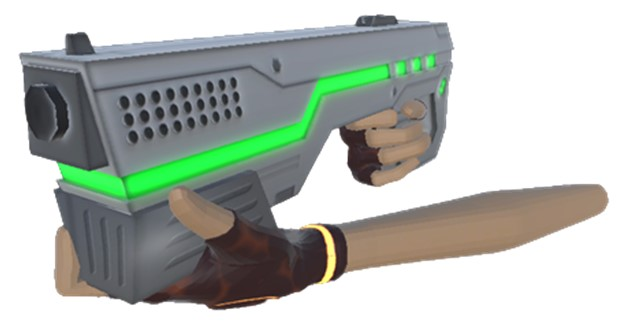
\includegraphics[scale=0.45]{img/Shotgun.jpg}
    \caption{Modelo completo de la escopeta en Unity}
    \label{fig:Escopeta}
    \end{figure}
    
    \item \textbf{\textit{Crear las animaciones del arma}}
    En este paso se deben crear todas las animaciones necesarias para el arma importada. También se pueden hacer en blender, como se ha hecho con otros objetos como las cajas de suministro, pero en este caso se ha preferido hacer directamente en Unity por conveniencia.\\
    En el caso de la escopeta, al igual que para el resto de armas, las animaciones necesarias son la que se ve al sacar el arma para utilizarla y la de recargar (ver figura \ref{fig:AnimacionEscopeta}), además de una adicional para cuando el arma esté en estado nuetro (sin hacer ninguna acción).
    
    Cabe mencionar que la acción de disparar se anima de forma procedural por código, por lo que no es necesario crear una animación específica de disparo (esto se explica más a fondo en la sección \textit{Aspectos relevantes del proyecto} de la memoria.
    \begin{figure}[h]
    \centering
    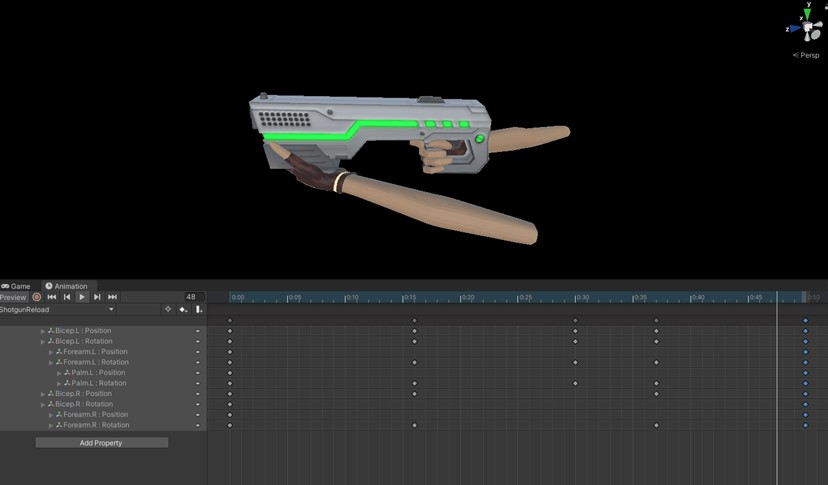
\includegraphics[scale=0.45]{img/ReloadingShotgun.jpg}
    \caption{Proceso de animación de recarga para la escopeta}
    \label{fig:AnimacionEscopeta}
    \end{figure}
    Una vez creadas todas las animaciones, se configura un nuevo \textbf{\textit{Animator Controller}}, que se encargará de supervisar el flujo y la transición de las animaciones en el orden y momento adecuados a través de una \textbf{\textit{State Machine}} o Máquina de estados (ver figuras \ref{fig:AnimatorEscopeta} y \ref{fig:EstadosEscopeta}).
    
    Por ejemplo, cuando el jugador tenga equipada el arma, no tenga el cargador lleno y pulse la tecla ``R'', se reproducirá la animación de recarga para que el jugador obtenga un feedback visual de la acción.
    
    \begin{figure}[h]
    \centering
    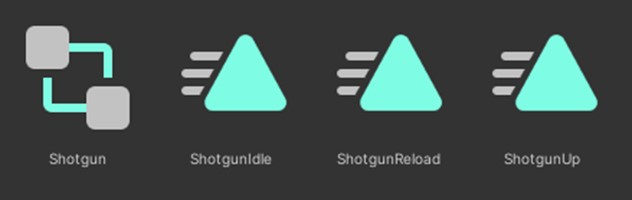
\includegraphics[scale=0.45]{img/ShotgunAnimatorController.jpg}
    \caption{Animator y animaciones de la escopeta}
    \label{fig:AnimatorEscopeta}
    \end{figure}
    
    \begin{figure}[h]
    \centering
    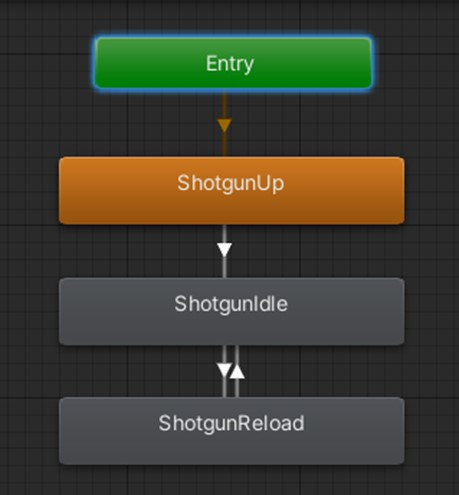
\includegraphics[scale=0.45]{img/StateMachine.jpg}
    \caption{Máquina de estados de las animaciones de la escopeta}
    \label{fig:EstadosEscopeta}
    \end{figure}
    
    \item \textbf{\textit{Crear scriptableObject del arma}}
    Ahora que ya se tienen listos todos los recursos visuales y sonoros del arma, se empieza a generar la lógica de esta. Para seguir con el flujo de datos diseñado para la lógica de las armas, se debe crear un scriptableobjet asociado a la escopeta. En este caso se utiliza la plantilla \textbf{\textit{WeaponBlueprint}} como modelo, que añade la opción ``Weapon'' al menú de creación de assets para este fin (ver figura \ref{fig:CrearArmaScriptableObject}).
    
    \begin{figure}[h]
    \centering
    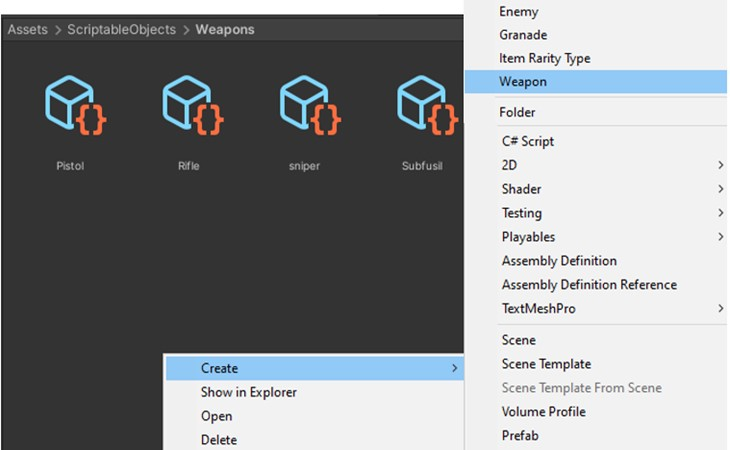
\includegraphics[scale=0.45]{img/NewWeapon.jpg}
    \caption{Crear un nuevo tipo de arma a través de un scriptableObject}
    \label{fig:CrearArmaScriptableObject}
    \end{figure}
    
    \item \textbf{\textit{Rellenar datos estáticos del arma}}
    Una vez creado el scriptableObject, se rellena con las propiedades, estadísticas y atributos del arma, como su daño, su alcance, su tiempo de recarga o las pistas de audio correspondientes que se crearon al principio (ver figura \ref{fig:PropiedadesEscopeta}).
    
    \begin{figure}[h]
    \centering
    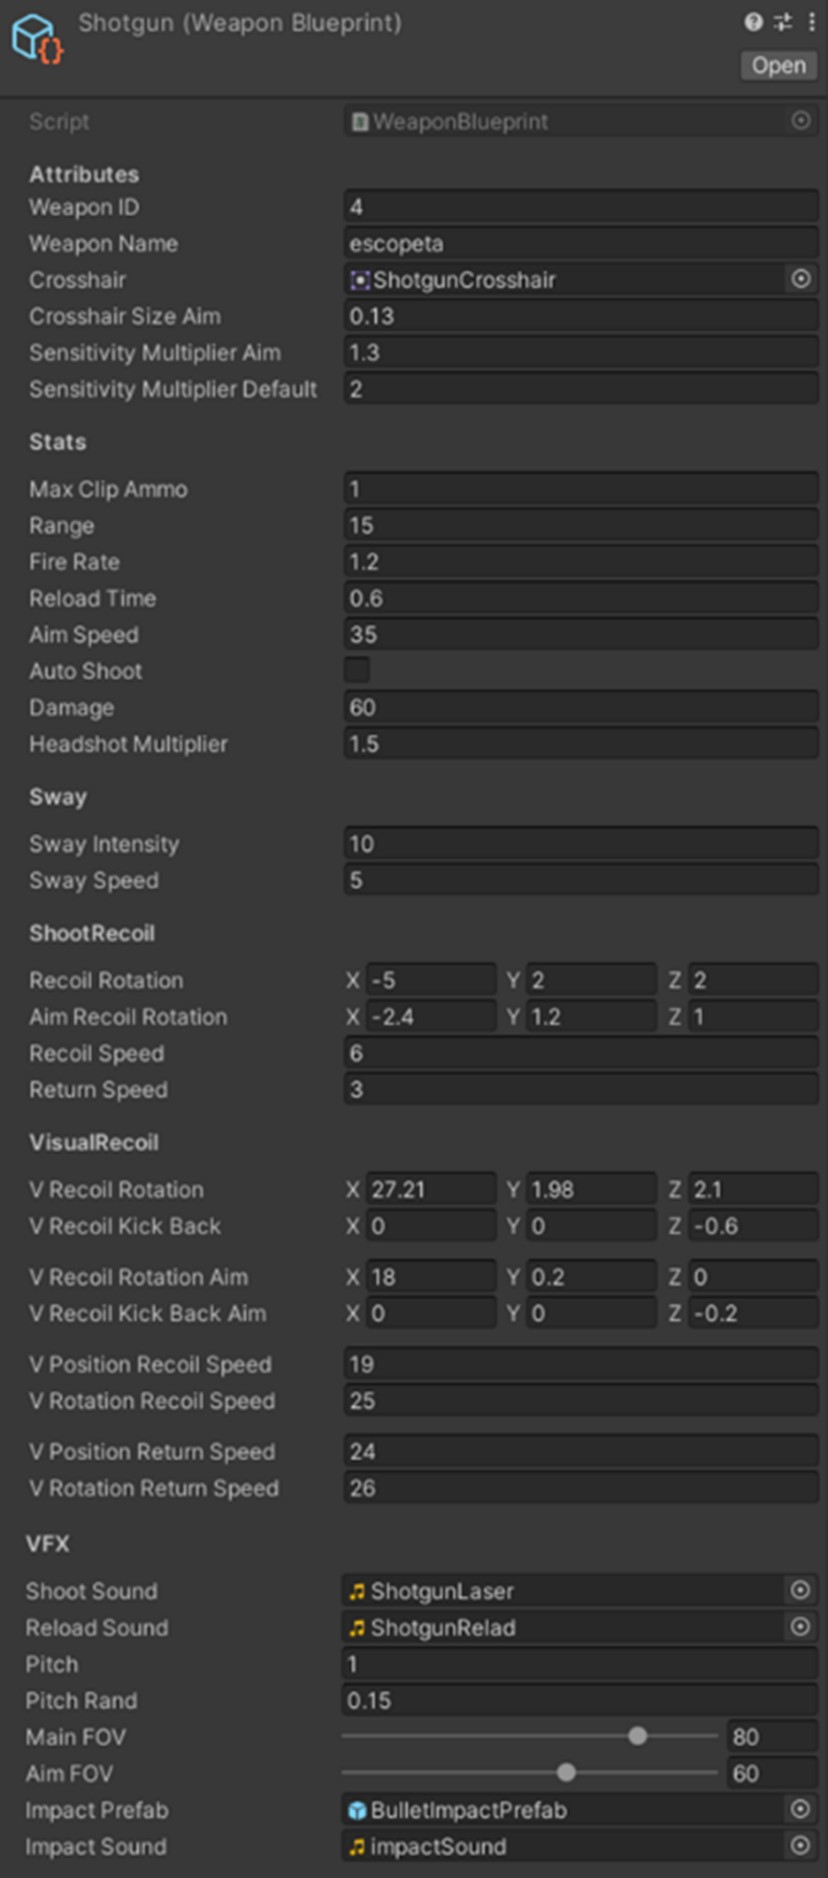
\includegraphics[scale=0.5]{img/ShotgunProperties.jpg}
    \caption{Propiedades y atributos de la escopeta}
    \label{fig:PropiedadesEscopeta}
    \end{figure}
    
    \item \textbf{\textit{Rellenar datos estáticos del arma}}
    Una vez creado el scriptableObject general del arma, hay que crear otros, esta vez a partir de la clase \textbf{\textit{ItemRarityBlueprint}}, para definir las propiedades y referencias de las distintas rarezas de la escopeta (ver figura \ref{fig:ScriptableObjectRarezas}). Entre ellas destacan: el modelo creado para representar cada rareza, el multiplicador de daño propio de cada una, la probabilidad que tiene un arma de dicha rareza de aparecer en cajas o cuándo se elimina a un enemigo.\\
    También contiene aspectos visuales, como los elementos que forman la etiqueta que aparece cuando el jugador mira hacia el arma, o el color y el icono del inventario cuando se equipa.
    
    \begin{figure}[h]
    \centering
    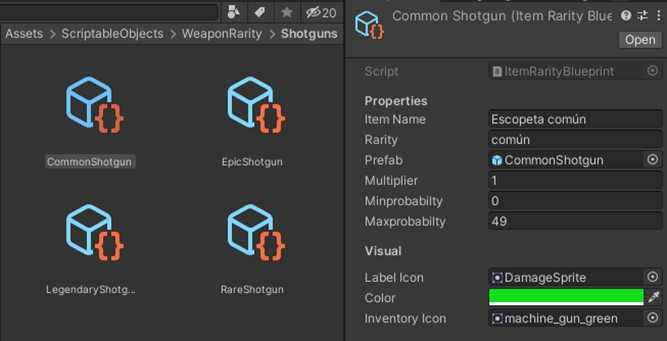
\includegraphics[scale=0.45]{img/CommonShotgunRarity.jpg}
    \caption{ScriptableObjects de las rarezas de la escopeta}
    \label{fig:ScriptableObjectRarezas}
    \end{figure}
    
    \item \textbf{\textit{Añadir el código necesario}}
     En el \textit{GameManager}, se deben añadir el conjunto de scriptableobjects de las rarezas para que pueda tener referencias a ellas al instanciar una escopeta. Asimisimo, en la clase \textit{Weapon}, propia de todas las armas, se debe incluir el caso de la escopeta al generar un arma, así como determinar su rareza desde el \textit{GamManager} en función de la probabilidad definida anteriormente para cada una de ellas (ver figuras \ref{fig:CodigoRarezasGameManager} y \ref{fig:CodigoRarezasWeapon}).
     
     \begin{figure}[h]
    \centering
    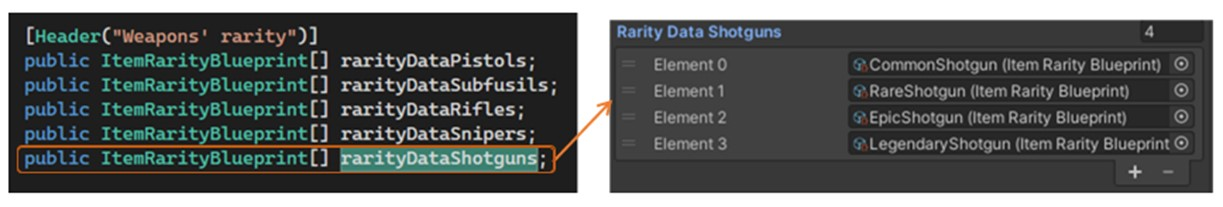
\includegraphics[scale=0.45]{img/ShotgunRarity.jpg}
    \caption{Código añadido en la clase \textit{GameManager} referente a las rarezas de la escopeta}
    \label{fig:CodigoRarezasGameManager}
    \end{figure}
    
    \begin{figure}[h]
    \centering
    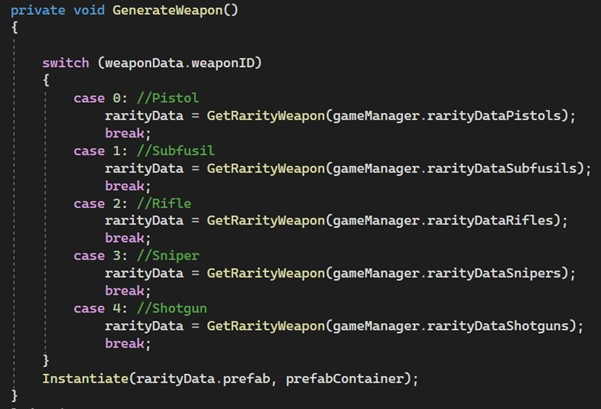
\includegraphics[scale=0.5]{img/GenerateWeapon.jpg}
    \caption{Código añadido a la clase \textit{Weapon} para crear la escopeta}
    \label{fig:CodigoRarezasWeapon}
    \end{figure}
    
     \item \textbf{\textit{Crear el Prefab de la escopeta}}
     El último paso es crear un \textbf{\textit{prefab}} que unifique todo lo anterior (ver figura \ref{fig:PrefabEscopeta}). Se le debe añadir el componente \textit{Weapon}, añadiendo el scriptableObject general de la escopeta en la variable ``WeaponData''.
     
     \begin{figure}[h]
    \centering
    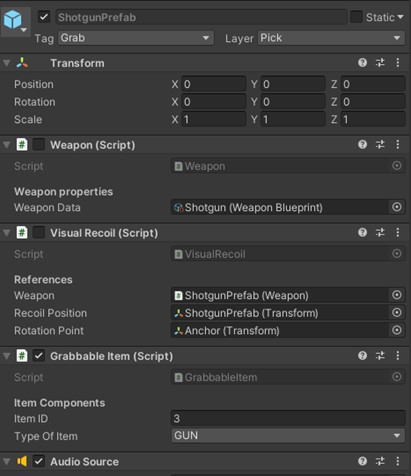
\includegraphics[scale=0.5]{img/ShotgunPrefab.jpg}
    \caption{Prefab de la escopeta}
    \label{fig:PrefabEscopeta}
    \end{figure}
    
\end{enumerate}
Este flujo de trabajo se puede extrapolar, aunque con salvedades en algunos pasos y con variaciones en ciertos componentes, al diseño y creación de otros datos y elementos del sistema, como, por ejemplo, el resto de armas, las granadas, los packs de ayuda o los enemigos.

\subsection{Diseño del inventario}
Una de las piezas centrales del videojuego es el inventario del personaje. A ojos del jugador, funcionará como una “mochila” en la que guardar objetos que se encuentre a su paso para poder usarlos de manera estratégica cuando considere conveniente.
Su diseño está configurado de la siguiente manera:

Se ha implementado la clase \textbf{\textit{InventorySlot}}, que representa cada uno de los espacios o compartimentos que tiene el inventario.

Internamente, cada slot funciona como una \textbf{pila de objetos} del tipo \textit{GrabbableItem}, es decir de los objetos que el jugador puede equiparse. La pila implementa las funciones propias de este tipo de estructuras, como las que permiten apilar (\textit{push}) un nuevo objeto, así como eliminar (\textit{pop}) o ver (\textit{peek}) el objeto de la cima de la pila, entre otras. Estas funciones están asociadas a ciertas acciones que hace el jugador durante la partida, como recoger o tirar un objeto.\\
También tiene otras funciones como, por ejemplo, comprobar, antes de apilar un objeto en un slot no vacío, que es compatible con el o los objetos que ya estén en la pila (\textbf{\textit{IsStackable}}).

Actualmente solo las granadas pueden apilarse en un mismo slot para así ahorrar espacio al jugador y que pueda llevar tantas granadas como se encuentre sin preocuparse de que se quede sin espacio en el inventario.

El inventario del jugador es una estructura de datos en forma de lista de slots, es decir, de instancias de la clase InventorySlot. En la figura \ref{fig:EstrucuraInventario} se puede ver la estructura general del inventario. Gestiona todos los objetos incluidos o potenciales de ser incluidos en él, controlando cuándo añadir o soltar un objeto del inventario, en qué slot debe ir cada objeto, o qué slot y, por tanto, qué objeto, debe estar activo en cada momento según el input del usuario.

\begin{figure}[h]
    \centering
    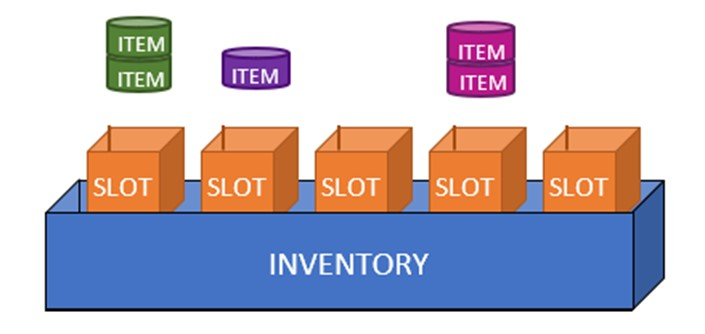
\includegraphics[scale=0.5]{img/InventoryScheme.jpg}
    \caption{Esquema de la estructura del inventario}
    \label{fig:EstrucuraInventario}
    \end{figure}
    
Además, como se ha mencionado en el apartado ``Events'' \ref{Events}, se utiliza la clase \textbf{\textit{InventoryVisuals}} para gestionar toda la parte audiovisual del inventario, manteniéndola separada de la lógica real.\\
Se encarga de mostrar por medio de una interfaz, los espacios del inventario, a través de imágenes en forma romboidal.\\
Cada uno de ellos tendrá una imagen de la clase de objetos que contiene dicho espacio en la parte lógica en caso de no estar vacío. Asimismo, pintará tanto el borde como el fondo del espacio de un color según el tipo o la rareza del objeto, y hará que el espacio o slot activo sea más grande que el resto para que el jugador sepa qué arma o granada puede usar en cada momento (ver figura \ref{fig:InterfazInventario}). Todo ello acompañado de efectos de sonido cuando el jugador cambie de objeto activo, lo tire al suelo o recoja alguno del suelo.

\begin{figure}[h]
    \centering
    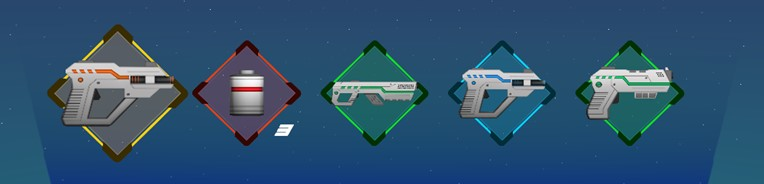
\includegraphics[scale=0.55]{img/InventoryInterface.jpg}
    \caption{Interfaz del inventario en uso}
    \label{fig:InterfazInventario}
    \end{figure}
    
De esta forma se consigue diseñar una estructura de datos que pueda gestionar adecuadamente todos los objetos que el jugador tenga equipados. Así, a un alto nivel, será sencillo y natural para el jugador recoger, tirar, usar o cambiar de arma y que haya un feedback audiovisual claro de estas acciones (ver diagrama de clases en la figura \ref{fig:InventarioUML})

\begin{figure}[h]
    \centering
    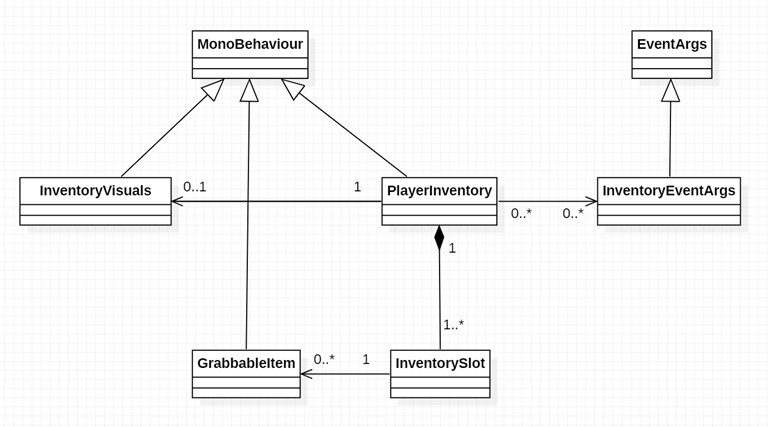
\includegraphics[scale=0.45]{img/InventoryClassDiagram.jpg}
    \caption{Diagrama de clases del inventario del jugador}
    \label{fig:InventarioUML}
    \end{figure}
    
\subsection{Diseño de interfaces}
El diseño de las interfaces de la aplicación es una parte fundamental del proyecto para asegurar el buen uso del videojuego, además de ser un elemento estético importante que conecta visualmente al resto de elementos. Es la forma en la que usuario y sistema se comunican durante gran parte del tiempo y, por ello, la experiencia de usuario al navegar o interactuar con cualquiera de las pantallas debe ser fluida, intuitiva y clara.

Se han utilizado varios elementos para conseguir esta facilidad de uso de las interfaces. Por ejemplo, se han escogido colores vivos, tipografías con un estilo futurista pero fáciles de leer, con un tamaño adecuado y botones grandes y descriptivos.

Se ha intentado mantener un cierto minimalismo en la composición visual, así como una armonía estética, haciendo uso de colores complementarios, degradados, y contrastando los elementos importantes, como el texto y los botones con el fondo. También se ha intentado dar énfasis a algunos elementos utilizando el color o el tamaño, como se puede apreciar (ver figura \ref{fig:InterfacesManuRegistro}), por ejemplo, en el menú principal, donde el botón de ``jugar'' es más grande que el resto para darle una importancia mayor y el botón de ``salir'' tiene un color rojizo para indicar alerta.

\begin{figure}[h]
    \centering
    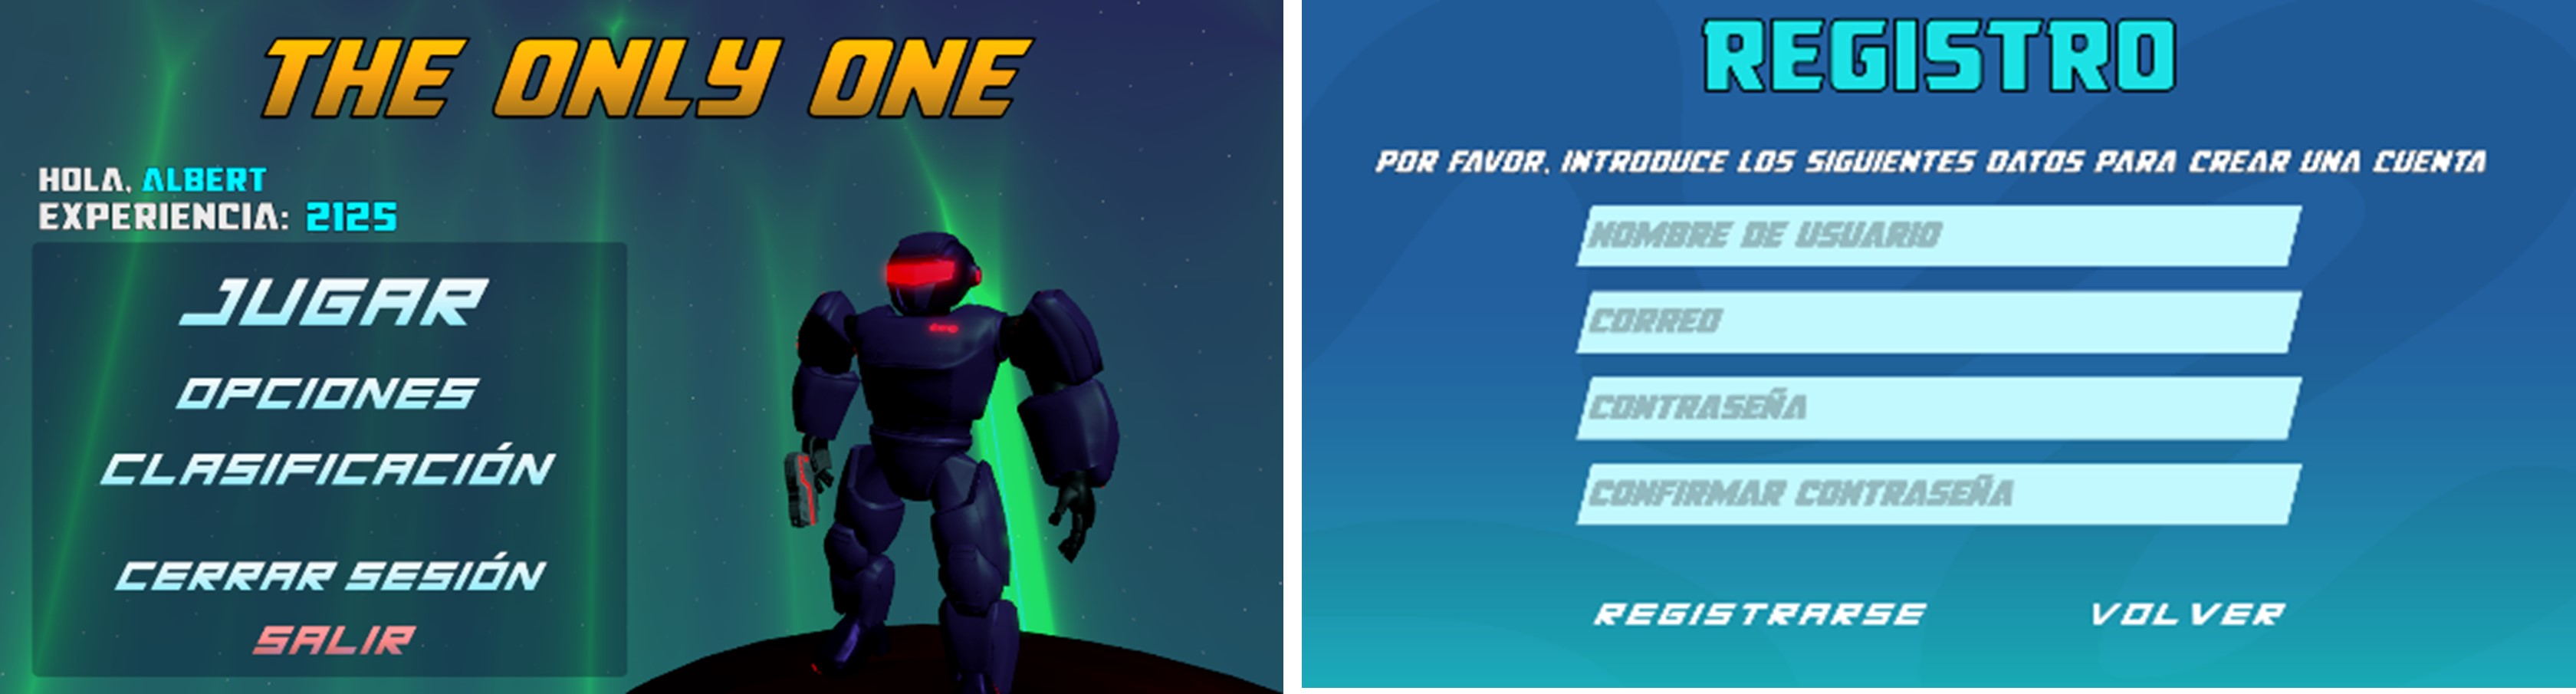
\includegraphics[scale=0.45]{img/Interfaces.jpg}
    \caption{Interfaces del menú principal y de registro}
    \label{fig:InterfacesManuRegistro}
    \end{figure}
    
Hay que mencionar también la existencia de una \textbf{pantalla de carga} que se muestra en las transiciones entre escenas, que es cuando más tiempo toma la aplicación para cargar los elementos. De esta forma, el jugador recibe en todo momento algún tipo de feedback del estado de la aplicación, evitando así que piense que la aplicación se ha congelado, está en algún estado de error al ver una pantalla negra o que no responde a su input.

En ella se puede ver la nube tóxica desde lejos a modo de fondo, así como el título del videojuego, junto a un pequeño eslogan. También se incluye una rueda de carga que gira continuamente, y la palabra ``cargando…'' para informar al usuario de que la escena está en proceso de carga (ver figura \ref{fig:PantallaDeCarga}).

\begin{figure}[h]
    \centering
    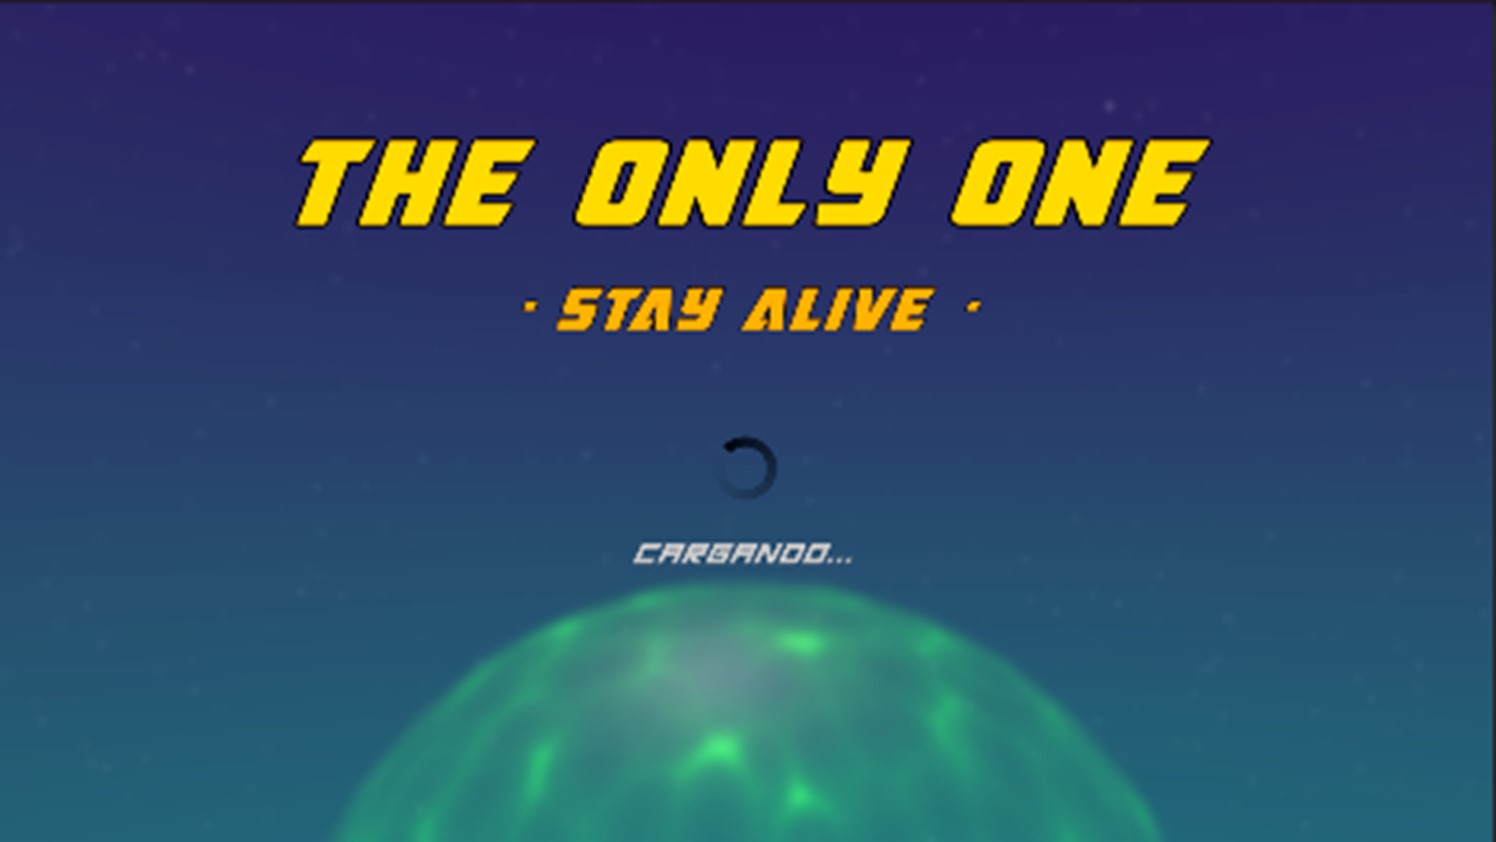
\includegraphics[scale=0.45]{img/LoadingScreen.jpg}
    \caption{Pantalla de carga del videojuego}
    \label{fig:PantallaDeCarga}
    \end{figure}
    
Finalmente, para el diseño del \textbf{logo del videojuego} se ha utilizado el software de edición de vectores llamado Illustrator, y se han querido reflejar en él algunos de los elementos del videojuego, como la cabeza de los enemigos, que además sirve como letra “O” para completar el título del videojuego o la corona que simboliza la victoria. Todo esto enmarcado en un círculo que simboliza la zona segura del mapa (ver figura \ref{fig:Logo}).

\begin{figure}[h]
    \centering
    
\includegraphics[scale=0.45]{img/Logo_TheOnlyOne.png}
    \caption{Logo del videojuego ``The Only One''}
    \label{fig:Logo}
    \end{figure}

\section{Diseño procedimental}
Una vez visto cómo se han diseñado los datos principales de la aplicación para poder construirla, se analizarán ahora los flujos de ejecución de los datos descritos en tiempo de ejecución para entender de qué manera funcionan los procesos y los estados de los componentes del videojuego.

\subsection{Flujo de autenticación e interacción con la base de datos}
La autenticación de un usuario de la aplicación es un proceso que integra varios pasos, entre los que destaca la interacción con la base de datos conectada a la aplicación.

El sistema hará operaciones de lectura y escritura en la base de datos en función de la información que requiera actualizar o solicitar.

En la figura \ref{fig:DiagramaBBDD} se puede ver, a grandes rasgos, el conjunto de secuencias de datos que hay entre el usuario, la aplicación y la base de datos, desde que el usuario se registra hasta que termina una partida y puede ver su experiencia reflejada en la interfaz del menú principal. Se ha elaborado el diagrama sobre dicha secuencia de acciones porque incluye todas las peticiones y respuestas posibles con la base de datos.

\begin{figure}[h]
    \centering
    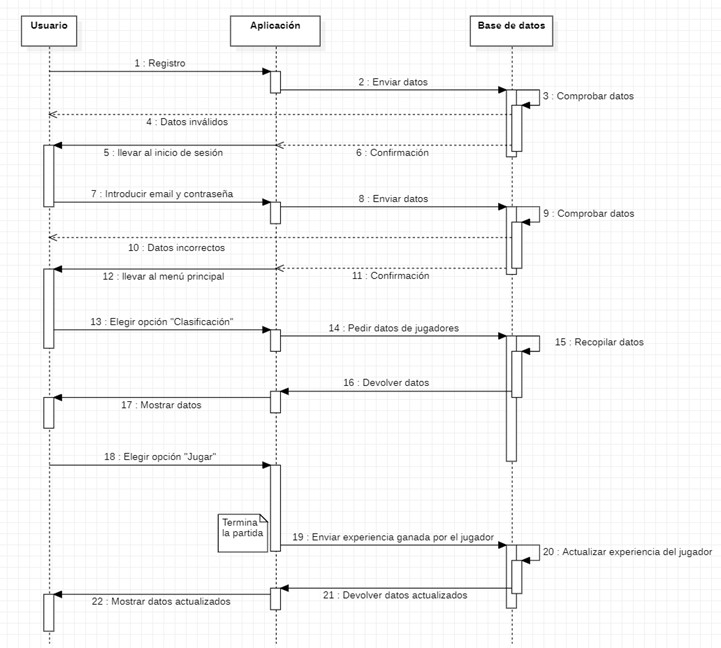
\includegraphics[scale=0.55]{img/DatabaseUsageFlowchart.jpg}
    \caption{Diagrama de secuencia del uso de la base de datos}
    \label{fig:DiagramaBBDD}
    \end{figure}

\subsection{Estados del jugador}
El jugador, a lo largo de la partida, puede pasar por diferentes estados según las situaciones que ocurran o las acciones que tome el usuario como input. En la figura \ref{fig:EstadosJugador} se reflejan los distintos estados con relación a su \textbf{movimiento}.\\
Cabe destacar que, desde cualquiera de ellos, se puede recibir daño, morir o ganar la partida. Son estados que no se incluyen en el diagrama por su trivialidad.

\begin{figure}[h]
    \centering
    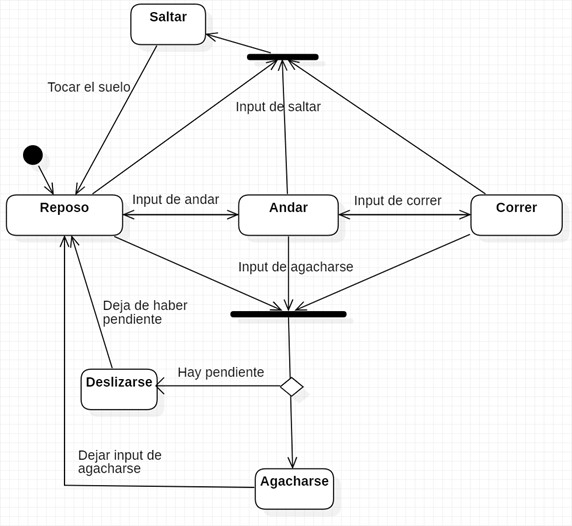
\includegraphics[scale=0.5]{img/PlayerStatesDiagram.jpg}
    \caption{Diagrama de estados del jugador}
    \label{fig:EstadosJugador}
    \end{figure}

\subsection{Salud del jugador}
Para entender el funcionamiento del sistema de salud del jugador, se representa en los siguientes diagramas el flujo de ejecución de sus diferentes componentes (ver figuras \ref{fig:DiagramaCuracion}, \ref{fig:DiagramaArmadura} y \ref{fig:DiagramaDaño}).

\begin{figure}[h]
    \centering
    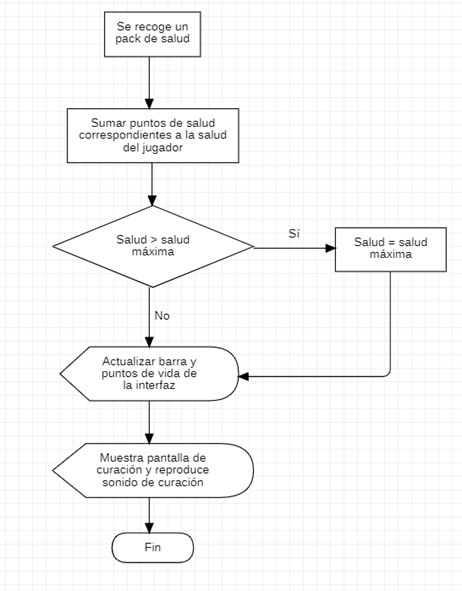
\includegraphics[scale=0.5]{img/HealingFlowchart.jpg}
    \caption{Diagrama de flujo de curación}
    \label{fig:DiagramaCuracion}
    \end{figure}
    
\begin{figure}[h]
    \centering
    \includegraphics[scale=0.5]{img/ArmorRecoveryFlowchart.jpg}
    \caption{Diagrama de flujo de recuperación de armadura}
    \label{fig:DiagramaArmadura}
    \end{figure}
    
\begin{figure}[h]
    \centering
    \includegraphics[scale=0.5]{img/DamageFlowchart.jpg}
    \caption{Diagrama de flujo de recibir daño}
    \label{fig:DiagramaDaño}
    \end{figure}

\subsection{Estados del enemigo}
Para generar un comportamiento verosímil de los enemigos, se ha desarrollado un sistema que trata de simular el comportamiento real de un jugador.  De acuerdo con esto, su funcionamiento se ha diseñado como una \textbf{máquina de estados} en la que, dependiendo en qué condición se encuentre, podrá realizar unas acciones u otras. Estas situaciones llevarán al enemigo a encontrarse en diferentes estados a medida que avanza el transcurso de la partida, todo ello en tiempo real.

En la figura \ref{fig:DiagramaEnemigo} se muestra el diagrama que representa los estados y las condiciones para pasar de unos a otros (los estados en azul son en movimiento, mientras que los naranjas son estáticos):

\begin{figure}[h]
    \centering
    \includegraphics[scale=0.45]{img/EnemyStates.jpg}
    \caption{Diagrama de estados del enemigo}
    \label{fig:DiagramaEnemigo}
    \end{figure}
    
\subsection{Añadir un objeto al inventario}
Uno de los aspectos a destacar del proyecto es el modo en que funciona el inventario del jugador. Para visualizar el procedimiento que se sigue a la hora de coger un objeto y hacer que se asigne de manera correcta y ordenada en el inventario, se muestra a modo de esquema, en la figura \ref{fig:DiagramaRecogerObjeto}, un diagrama donde se visualizan las principales acciones y comprobaciones que ocurren, desde que el jugador pulsa la tecla de recoger el objeto hasta que lo tiene equipado, listo para usarse, incluyendo feedback visual.

\begin{figure}[h]
    \centering
    \includegraphics[scale=0.5]{img/PickingObjectFlowchart.jpg}
    \caption{Diagrama de flujo de recoger un objeto}
    \label{fig:DiagramaRecogerObjeto}
    \end{figure}

\subsection{Flujo de escenas e interfaces}
Con el objetivo de visualizar mejor todas las interfaces que componen el videojuego, se ha creado un esquema (ver figura \ref{fig:DiagramaPantallas}) a modo de diagrama que representa el flujo de ejecución de la aplicación a través de la interconexión entre ellas.

\begin{figure}[h]
    \centering
    \includegraphics[scale=0.4]{img/ScreenFlowChart.png}
    \caption{Diagrama de flujo entre pantallas}
    \label{fig:DiagramaPantallas}
    \end{figure}
    
\section{Diseño arquitectónico}
En este apartado se analizará la estructura general de la aplicación como software creado dentro de un motor de videojuegos, así como el modo en el que se relaciona con otras entidades, como la base de datos, las diferentes librerías que utiliza o los paquetes usados en la aplicación.

El controlador que gestiona todos los paquetes de la aplicación es el llamadado \textbf{\textit{Package Manager}} \cite{doc:PackageManager} o Controlador de paquetes. Es un contenedor proporcionado por Unity para almacenar varios tipos de archivos y características, como librerías, frameworks, o dependencias del proyecto.

Algunos de los paquetes internos que utiliza este proyecto son los que se listan en la  figura \ref{fig:Paquetes internos}:
\begin{figure}[h]
    \centering
    \includegraphics[scale=0.45]{img/PackagesUnity.png}
    \caption{Paquetes internos de Unity en el proyecto}
    \label{fig:Paquetes internos}
    \end{figure}
    
Por ejemplo, el paquete ``Shader Graph'' añade a Unity un editor visual de shaders, que se ha utilizado para crear algunos de los shaders del proyecto, como el de la nube tóxica, el rastro de las granadas o el cielo. Otro paquete digno de mencionar es \textit{TextMeshPro}. Este paquete incluye todo un conjunto de herramientas para crear textos de calidad en el proyecto. De hecho, todos los textos que se pueden ver en la aplicación están creados con esta librería.

Algunos paquetes ofrecen funcionalidades añadidas y opcionales, como los descritos anteriormente, pero otros son fundamentales para que la aplicación funcione correctamente a nivel interno, como el paquete de Servicios \textit{Services Core}, que define los componentes comunes de los \textit{Game Services Packages}.

Existen otro tipo de paquetes externos, añadidos por el desarrollador, que se han importado al proyecto desde la \textit{Unity Asset Store}. Estos son:
\begin{itemize}
    \item \textbf{2D Sci-Fi Weapon Pack}: paquete de imágenes destinadas a representar los iconos de las armas y las granadas en el inventario.
    \item \textbf{Sci-Fi Weapons Pack}: paquete de modelos 3D de las armas base utilizadas, así como sus texturas.
    \item \textbf{Quick Outline}: librería utilizada para colorear el borde de los objetos cuando se puede interactuar con ellos.
    \item \textbf{Robot Soldier}: modelo 3D del robot utilizado como enemigo.
    \item \textbf{Lean Tween}: librería para animar elementos de la interfaz, empleada cuando el jugador mata a un enemigo y cuando aparece la pantalla del resumen de la experiencia ganada al final de la partida.
\end{itemize}
Cuando Unity carga un proyecto, el Package Manager lee el \textbf{\textit{Project manifest}} para comprobar una lista de paquetes y dependencias que debe recuperar y cargar. Es un archivo en formato JSON que se actualiza cuando, por ejemplo, el desarrollador instala o desinstala un paquete externo.

El archivo \textit{manifest.json}, al momento de compilar la aplicación final, se ve como en la figura \ref{fig:ManifestJSON}:

\begin{figure}[h]
    \centering
    \includegraphics[scale=0.45]{img/Manifestjson.jpg}
    \caption{Archivo manifest.json}
    \label{fig:ManifestJSON}
    \end{figure}
    
La forma en la que Unity integra los paquetes es la siguiente (ver figura \ref{fig:FlujoPaquetes}):

\begin{enumerate}
    \item Al abrir un proyecto, el package manager lee el manifest.json para saber qué paquetes cargar.
    \item Envía una petición al package registry server o servidor de registro de paquetes por cada paquete que aparezca como dependencia en el archivo manifest
    \item El registro de paquetes envía la información solicitada de vuelta al package manager.
    \item El package manager instala los paquetes en el proyecto.
\end{enumerate}

\begin{figure}[h]
    \centering
    \includegraphics[scale=0.45]{img/PackageManagerFlowchart.jpg}
    \caption{Flujo de peticiones de paquetes}
    \label{fig:FlujoPaquetes}
    \end{figure}

Cuando se instala un paquete desde el \textit{Package Manager}, realmente se están añadiendo dependencias al archivo manifest.json. Con ello se especifica la versión particular del paquete que se necesita para que el proyecto funcione como se espera. Estas dependencias que aparecen en el Project manifest se denominan dependencias directas.

Sin embargo, los paquetes puede que necesiten de otros paquetes para que funcionen. Estas serían las dependencias indirectas, y se deberían añadir de manera automática al instalar el paquete deseado. Si no lo hacen, se tienen que resolver esas dependencias manualmente o refrescando la importación.

Cuando el \textit{Package Manager} resuelve con éxito todas las versiones adecuadas de las dependencias, se guarda esta resolución en un archivo llamado \textbf{\textit{packages-lock.json}}. Así se asegura la consistencia y la velocidad de carga de las dependencias cuando se carguen en el proyecto. En la figura \ref{fig:PaqueteLock} se puede ver un fragmento de su contenido:
\begin{figure}[h]
    \centering
    \includegraphics[scale=0.45]{img/Packages-lockJSON.jpg}
    \caption{Fragmento del archivo \textit{Packages-lock.json}}
    \label{fig:PaqueteLock}
    \end{figure}
Respecto a la base de datos a la que se conecta la aplicación, la estructura que sigue la conexión y el envío de datos se entiende mejor si se conoce cómo se ha implementado y cuál es su configuración.

Los pasos seguidos para integrar y conectar la aplicación a la base de datos en tiempo real de Firebase y para implementar la autenticación de usuarios fueron los siguientes:
\begin{enumerate}
    \item \textbf{Crear un proyecto de Firebase}: Un proyecto de Firebase es el contenedor de todos los servicios y recursos asociados a la aplicación a la que se conecta. Este proyecto, llamado ``TheOnlyOne'', por el momento, solamente utiliza los servicios de ``Authentication'' y ``Realtime Database'' para cubrir las necesidades requeridas (ver figura \ref{fig:JerarquíaFirebase}).
    
    \begin{figure}[h]
    \centering
    \includegraphics[scale=0.45]{img/HierarchyFirebaseProject.jpg}
    \caption{Esquema de la jerarquía de un proyecto de Firebase}
    \label{fig:JerarquíaFirebase}
    \end{figure}
    
    \item \textbf{Registrar la aplicación con Firebase}: En este paso se asocia cada versión que se vaya a compilar de la aplicación (Android, iOS…) al proyecto de Firebase, añadiendo el ID de del proyecto de Unity. En este caso, el ID de la aplicación para la plataforma Android es ``com.AlbertoFuente.TheOnlyOne''. 
    
    Si bien la aplicación no se ejecutará en Android, es la opción que se debe marcar para crear un proyecto de escritorio.
     \item \textbf{Agregar los archivos de configuración de Firebase}. En este paso se debe descargar un archivo llamado \textbf{\textit{google-services.json}} y añadirlo a la carpeta de assets del proyecto en Unity.
     
     Después se debe agregar el SDK de Firebase para Unity. Concretamente, se importan a Unity los paquetes que sean relevantes para el proyecto, así como las dependencias de estos para que puedan funcionar. En este caso, se añaden “FirebaseDatabase.unitypackage” para la configuración de la base de datos, y “FirebaseAuth.unitypackage” para la autenticación de usuarios. Antes de importar estos paquetes se debe comprobar qué versión de la librería .NET utiliza el proyecto, que en este caso es .NET 4.
    \item \textbf{Resolver las dependencias} de los paquetes importados desde el gestor de dependencias de Unity.
    \item \textbf{Crear la Base de datos}. En la consola de Firebase, crear la base de datos que utilizará el proyecto
    \item \textbf{Crear un método de autenticación de usuarios}: En la consola de Firebase, elegir el modo de acceso que se desea que utilicen los usuarios de la aplicación. En este proyecto se utiliza correo y contraseña como procedimiento de autenticación.
\end{enumerate}
Siguiendo todos estos pasos, ya estaría lista la configuración inicial de la base de datos y el método de autenticación de los usuarios para acceder a ella.

Como se puede observar en la figura \ref{fig:ManifestJSON}, que forma parte del archivo manifest.json, además de las dependencias, se puede ver un apartado llamado \textbf{\textit{Scoped Registries}}. Este tipo especial de registros permiten a Unity comunicar al package manager dónde se encuentra cada servidor de registro de paquetes. De esta forma, el usuario puede acceder a grandes colecciones de paquetes al mismo tiempo.

Al integrar la base de datos de Firebase con el proyecto de Unity, se instala automáticamente un Scoped Registry asociado a la API de Google para que la conexión con Firebase pueda producirse adecuadamente y se acceda a todos los paquetes necesarios (ver figura \ref{fig:ScopedRegistry}).
\begin{figure}[h]
    \centering
    \includegraphics[scale=0.45]{img/ScopedRegistry .jpg}
    \caption{\textit{Scoped registry} de Google}
    \label{fig:ScopedRegistry}
    \end{figure}



\apendice{Documentación técnica de programación}

\section{Introducción}
Durante este anexo se describirá con detalle la documentación técnica de programación del proyecto. Esto incluye aspectos como la estructura de directorios que tiene, la instalación y uso del entorno de desarrollo, cómo llevar a cabo tanto su compilación, su instalación y ejecución, así como el método seguido para realizar las diferentes pruebas durante el desarrollo.
\section{Estructura de directorios}
Todos los materiales que forman el proyecto se encuentran en el repositorio de Github. Los directorios y archivos que contiene se organizan según la estructura que se describe a continuación:
\begin{itemize}
    \item \textbf{/docs}: Contiene los archivos relativos a la documentación del proyecto.
    \item \textbf{/TheOnlyOne}: es el directorio raíz de la estructura del juego.
        \begin{itemize}
        \item \textbf{/TheOnlyOne/Assets}: Contiene todos los archivos del propio desarrollo del juego, como scripts, modelos, animaciones, escenas, materiales y demás componentes que se importan o se crean en el proyecto para construir el videojuego.
            \begin{itemize}
            \item \textbf{/TheOnlyOne/Assets/Animations}:Contiene todos los archivos relacionados con las animaciones del juego. Esto incluye tanto los \textit{Animator controllers}, como los  \textit{Animation Clips}. Se clasifican en subcarpetas según el tipo de animaciones.
            \item \textbf{/TheOnlyOne/Assets/Editor Default Resources}: Contiene archivos necesarios para los scripts que requieran recursos cargados bajo demanda. Es utilizado por la base de datos.
            \item \textbf{/TheOnlyOne/Assets/ExternalDependencyManager}: Contiene algunas dependencias de paquetes que en este caso son usadas por Google para que Firebase funcione correctamente
            \item \textbf{/TheOnlyOne/Assets/Firebase}: Contiene los archivos de configuración principales de la base de datos de Firebase.
            \item \textbf{/TheOnlyOne/Assets/Global Volumes}: Contiene los diferentes perfiles de postprocesado del videojuego.
            \item \textbf{/TheOnlyOne/Assets/LeanTween}: Contiene los archivos relacionados con el paquete externo \textit{LeanTween}, importado para crear animaciones en algunos elementos de la interfaz.
            \item \textbf{/TheOnlyOne/Assets/Materials}: Contiene los diferentes materiales usados en el videojuego. Se dividen en subcarpetas según el elemento al que se le aplique el material.
            \item \textbf{/TheOnlyOne/Assets/Meshes}: Contiene las mallas de los modelos 3D utilizados, tanto propios como importados.
            \item \textbf{/TheOnlyOne/Assets/Parse}: Contiene archivos relativos al framework dotNet45 para la conexión con Firebase.
            \item \textbf{/TheOnlyOne/Assets/PhysicsMaterials}: Contiene diferentes materiales físicos utilizados en el videojuego.
            \item \textbf{/TheOnlyOne/Assets/Plugins}: Contiene ficheros necesarios para el funcionamiento de la base de datos en dispositivos con sistema operativo iOS.
            \item \textbf{/TheOnlyOne/Assets/Firebase}: Contiene los archivos de configuración principales de la base de datos de Firebase.
            \item \textbf{/TheOnlyOne/Assets/Prefabs}: Contiene todos los prefabs usados en el videojuego. Se dividen en subcarpetas según el ámbito del Prefab.
                \begin{itemize}
                \item \textbf{/TheOnlyOne/Assets/Prefabs/FinalPrefabs}: Almacena los prefabs que se instancian directamente en la escena.
                \end{itemize}
            \item \textbf{/TheOnlyOne/Assets/Presets}: Contiene archivos de configuración por defecto generados por unity para audio e imágenes.
            \item \textbf{/TheOnlyOne/Assets/QuickOutline}: Contiene los archivos relativos al paquete externo “QuickOutline” importado para crear un efecto de borde resaltado a los objetos.
            \item \textbf{/TheOnlyOne/Assets/Sci-Weapon Pack}: Contiene los modelos, texturas, materiales y demás ficheros del paquete externo importado relativo a las armas y packs del juego.
            \item \textbf{/TheOnlyOne/Assets/Scenes}: Contiene todas las escenas que componen el videojuego.
            \item \textbf{/TheOnlyOne/Assets/ScriptableObjects}: Contiene los diferentes scriptableObjects del juego, subdivididos por tipo
            \item \textbf{/TheOnlyOne/Assets/Scripts}: 
            \begin{itemize}
                \item \textbf{/TheOnlyOne/Assets/Scripts/	ScriptableObjectsGenerator}: Contiene las clases que definen los scriptableobjects del juego.
                \item \textbf{/TheOnlyOne/Assets/Scripts/NavMeshComponents}: Contiene los scripts y otros componentes para hacer que los enemigos puedan caminar por el terreno como se espera.
            \end{itemize}
            \item \textbf{/TheOnlyOne/Assets/Settings}: Contiene archivos de configuración gráfica y visual del proyecto.
            \item \textbf{/TheOnlyOne/Assets/ShaderGraphs}: Contiene los distintos shaders creados para crear los materiales especiales que hay en el videojuego.
            \item \textbf{/TheOnlyOne/Assets/Sounds}: Contiene todas las pistas de audio que se utilizan en la aplicación.
            \begin{itemize}
                \item \textbf{/TheOnlyOne/Assets/Sounds/Music}: Contiene la música que se reproduce de fondo en el videojuego
                \item \textbf{/TheOnlyOne/Assets/Sounds/SoundFX}: Contiene los diferentes efectos de sonido que se reproducen durante la ejecución del juego.
                \item \textbf{/TheOnlyOne/Assets/Sounds/UI}: Contiene los sonidos que se reproducen al interactuar con la interfaz, como los botones.
            \end{itemize}
            \item \textbf{/TheOnlyOne/Assets/Sprites&Textures}: Contiene todas las imágenes del videojuego divididas en subcarpetas según el elemento al que pertenecen. Incluye texturas, sprites, y cualquier archivo de imagen que se utilice.
            \item \textbf{/TheOnlyOne/Assets/StreamingAssets}: Contiene archivos especiales que no se deben modificar cuando se acceda a ellos. Se utiliza para almacenar el archivo que permite utilizar la base de datos en la versión de escritorio del proyecto.
            \item \textbf{/TheOnlyOne/Assets/TextMeshPro}: Contiene los archivos de configuración del paquete “TextMeshPro”, así como las fuentes y demás recursos utilizados.
        \end{itemize}
        \item \textbf{TheOnlyOne/Packages}: Contiene los archivos de configuración de los paquetes de Unity.
        \item \textbf{TheOnlyOne/ProjectSettings}: Contiene los archivos de configuración del proyecto necesarios para que el proyecto se pueda cargar en Unity.
        \item \textbf{TheOnlyOne/UserSettings}: Contiene archivos de configuración del usuario.
        \end{itemize}
\end{itemize}
\section{Manual del programador}
En este apartado se detallarán algunos pasos y aspectos relevantes que debe conocer el programador para poder desarrollar, compilar y ejecutar el proyecto.
\subsection{Instalación de Unity}
Para poder cargar el proyecto adecuadamente, lo primero que se debe hacer es instalar el motor de videojuegos Unity. Este será la base para realizar el resto de acciones asociadas al desarrollo.

Para ello, primero se debe acceder a la página oficial de Unity y descargar \textbf{\textit{Unity Hub}} (ver figura \ref{fig:DescargarUnity}), un centro de control para la gestión de los proyectos y de las diferentes versiones de Unity.

Hay que tener en cuenta los requisitos del sistema que pide el software para que se pueda ejecutar sin problemas.

\begin{figure}[h]
    \centering
    \includegraphics[scale=0.45]{img/UnityDownload.jpg}
    \caption{Página oficial de descargas de Unity}
    \label{fig:DescargarUnity}
    \end{figure}
    
Una vez en Unity Hub, se debe empezar por instalar el editor de Unity. Es importante que la versión de Unity que se descargue sea la misma que se utilizó al desarrollarse por el alumno para evitar errores o inconsistencias. En este caso, la versión utilizada es la \textit{2020.3.23f1}.

Es posible utilizar una versión diferente a la comentada, pero Unity es sensible y propenso a errores en algunos componentes cuando se utilizan versiones diferentes en un mismo proyecto.

Para instalarla, se debe acceder al apartado ``Installs'', y pulsar en ``Install Editor''. Después se elige la versión de Unity que se desea instalar (ver figura \ref{fig:InstalarUnity}).

\begin{figure}[h]
    \centering
    \includegraphics[scale=0.45]{img/UnityInstall.jpg}
    \caption{Instalar Unity desde Unity Hub}
    \label{fig:InstalarUnity}
    \end{figure}
    
Al instalar cualquier versión, se muestran los distintos módulos que se pueden añadir a la instalación de Unity (ver figura \ref{fig:MódulosUnity}). Para este proyecto, son necesarios los \textbf{módulos de compilación} de Windows y de Linux para que se pueda ejecutar en estas plataformas, como se requiere en los requisitos.\\
También es posible agregar estos módulos posteriormente, una vez Unity esté instalado en el sistema.

\begin{figure}[h]
    \centering
    \includegraphics[scale=0.45]{img/UnityModules.jpg}
    \caption{Módulos de Unity}
    \label{fig:MódulosUnity}
    \end{figure}

\subsection{Importación del proyecto}
Unity hub permite añadir un proyecto nuevo o ya existente de varias formas. En este caso, lo que se debe hacer para importar el proyecto a Unity es descargarlo desde el repositorio de GitHub y guardarlo en algún directorio del ordenador.

Entonces en Unity Hub, en el apartado ``Projects'', se pulsa la opción de ``Open''. Se pedirá la ruta donde se encuentre el proyecto, y, una vez seleccionada, se añadirá el proyecto importado a la lista de proyectos disponibles (ver figura \ref{fig:ProyectosUnity}).

\begin{figure}[h]
    \centering
    \includegraphics[scale=0.45]{img/UnityProjects.jpg}
    \caption{Ver proyectos disponibles de Unity}
    \label{fig:ProyectosUnity}
    \end{figure}
    
Junto al nombre del proyecto, se puede ver la fecha de la última vez que se modificó el proyecto, y la versión de Unity que utiliza. Esta se puede modificar si se desea ejecutar con otra más adecuada.

Para abrir el proyecto simplemente se pulsa en su nombre, y, tras unos segundos de carga, se podrá empezar a trabajar con él.

\subsection{Editor de Unity}
Una vez se acceda al proyecto, se cargará el editor de Unity. Este se compone de varios elementos y ventanas que son importantes de conocer para poder desarrollar el proyecto adecuadamente.

Cabe destacar que las posición y dimensiones de las ventanas no son fijas, y se pueden mover y redimensionar libremente a gusto del desarrollador. 

\begin{figure}[h]
    \centering
    \includegraphics[scale=0.45]{img/UnityEditor.jpg}
    \caption{Editor de Unity}
    \label{fig:EditorUnity}
    \end{figure}
    
La figura \ref{fig:EditorUnity} sirve como leyenda para analizar cada una de las ventanas y elementos que más se utilizan en cualquier proyecto de Unity, descritos a continuación:
\begin{enumerate}
    \item \textbf{\textit{Scene}}. Esta ventana muestra un entorno 3D donde se pueden añadir los diferentes componentes disponibles para ir creando la escena. Dispone de una cámara virtual con la que se puede explorar este entorno libremente, alejándose o acercándose para examinar y editar cualquier elemento.\\
    Integra herramientas para modificar la posición, rotación y el tamaño de los gameobjects directamente desde la ventana.
    \item \textbf{\textit{Game}}. En la ventana de juego se muestra una vista previa de cómo se verá el juego una vez se ejecute. Resulta de gran valor para hacer pruebas de funcionamiento de las mecánicas o pruebas de disposición de los elementos de la interfaz.
    \item \textbf{\textit{Hierarchy}}. Es la jerarquía de objetos de la escena, es decir, esta ventana muestra todos los gameobjects y sus dependencias padre-hijo que existen dentro de la escena actual. Se puede utilizar para organizar y agrupar los gameobjects de la escena para gestionarlos más fácilmente.
    \item \textbf{\textit{Project}}. La ventana \textit{Project} contiene toda la jerarquía de assets y ficheros que se utilizan en el proyecto. Es una representación de la estructura de directorios y archivos que se almacena en disco relativa al proyecto, y contiene la información necesaria para poder cargarlo.
    
    Desde esta ventana se puede acceder a cualquier archivo del proyecto. Por ejemplo, se puede seleccionar cualquier escena dentro de la carpeta \textit{Assets/Scenes} para poder editarla. También se  puede utilizar para añadir elementos a la escena bien directamente como un gameobject o como componente de otros.\\
    Al arrastrar por ejemplo un Prefab desde esta ventana hasta la escena, se creará un nuevo gameobject en la Hierarchy, y ese gameobject ya formará parte de la escena.
    \item \textbf{\textit{Inspector}}. Esta ventana muestra toda la información y componentes de un objeto seleccionado, tanto de la \textit{Hierarchy} como de la carpeta Assets. Esta ventana permite ver las propiedades del objeto, añadir o eliminar componentes, activar o desactivarlos, o modificar sus valores.
    \item \textbf{\textit{Console}}. La consola de Unity funciona como cualquier consola de un entorno de desarrollo de software, mostrando todos los mensajes, las advertencias y los errores pertinentes que puedan surgir.\\
    Resulta de gran ayuda para depurar scripts, por ejemplo, ya que suele indicar la línea concreta en la que se encuentra el error, y cómo se ocasionó.
\end{enumerate}
De forma complementaria a las principales ventanas del editor, para poder editar y crear nuevos scripts, es recomendable disponer de un \textbf{IDE de programación} apropiado.

En el caso de Unity, lo habitual es utilizar \textit{Visual Studio}, ya que tiene varias funcionalidades para el desarrollo en Unity, como funciones de autocompletado o de depuración.\\
Para asociarlos, una vez en el proyecto, se debe seguir la ruta \textit{Edit>Preferences>External Tools}, y en la opción \textit{External Script Editor}, seleccionar el editor instalado en el ordenador que se desee utilizar (ver figura \ref{fig:HerramientasExternas}). En este caso, el editor y la versión elegidos ha sido Visual Studio Community 2022.

\begin{figure}[h]
    \centering
    \includegraphics[scale=0.45]{img/ExternalTools.jpg}
    \caption{Asociar el proyecto a un IDE de programación}
    \label{fig:HerramientasExternas}
    \end{figure}
    
Una vez hecho esto, para editar un script basta con hacer doble clic sobre él, y automáticamente se abrirá Visual Studio para poder editarlo fácilmente. Al guardar los cambios realizados en el script, este se compilará de forma automática, y, si hay algún error o advertencia relacionados con el script, se mostrará en la consola del editor.

\section{Compilación, instalación y ejecución del proyecto}
Una vez se da por finalizado el desarrollo del videojuego, se debe compilar para poder exportarlo y ejecutarlo en otros dispositivos.
Para que la aplicación se compile en un producto final, simplemente hay que dirigirse al apartado \textit{Build Settings} dentro de la opción \textbf{File} del editor. 

Se abrirá una ventana de configuración (ver figura \ref{fig:OpcionesCompilacion}) donde se deben añadir todas las escenas que formen el juego. Es importante definir bien el orden en que se añaden estas escenas, ya que se les asignará un índice diferente a cada una en función del orden que sigan en esta ventana. 
\\
Esto será relevante a la hora de referenciar a las escenas en los scripts y porque la escena con el índice 0 será la primera en cargarse cuando se ejecute la aplicación.

\begin{figure}[h]
    \centering
    \includegraphics[scale=0.45]{img/BuildSettings.jpg}
    \caption{Opciones de compilación}
    \label{fig:OpcionesCompilacion}
    \end{figure}
    
Tras añadir las escenas en orden, se debe definir la plataforma para la que se desea compilar la aplicación, y, en su caso, el sistema operativo objetivo. Además, se pueden ajustar otras opciones como el tipo de arquitectura, o si se desea crear la solución para visual studio.
Una vez se seleccionen las opciones deseadas, simplemente se debe pulsar en ``Build'' para escoger el directorio donde se exportará el juego, almacenando todos los archivos necesarios para ejecutarlo (ver figura \ref{fig:FicherosJuego}).

\begin{figure}[h]
    \centering
    \includegraphics[scale=0.45]{img/GeneratedFiles.jpg}
    \caption{Ficheros generados en la compilación del juego}
    \label{fig:FicherosJuego}
    \end{figure}

\section{Pruebas del sistema}
Todo proyecto necesita hacer pruebas y testeos sobre sus diferentes componentes, así como del producto final, para comprobar que todo funciona como debe o si hay que hacer modificaciones en algunos elementos para tal fin.

La forma en la que se han puesto a prueba los elementos del videojuego es sencilla y ágil, permitiendo introducir cambios de forma conveniente en cada momento.
El editor de Unity permite ejecutar en cualquier momento la escena actual (siempre que no haya errores en los scripts), pulsando el botón \textbf{``Play''} de la parte superior del editor. 

Cuando se desea probar un elemento o parte de un elemento cuyo desarrollo se da por completado, se añade a la escena y se pulsa ``Play''. El usuario, a través de la ventana ``Game'', puede interactuar con el elemento como lo haría una vez se compilase el juego, para combropar que todo funciona como espera. Además, se puede complementar con el uso de la ventana ``Scene'', donde, incluso en tiempo de ejecución, el usuario puede navegar con la cámara virtual y seleccionar cada parte del elemento que se esté probando para ver en el Inspector si sus valores son los adecuados en cada momento.

Así, se testea de forma interactiva cada elemento que se quiera introducir de forma definitiva en la aplicación. Además, no hay que probar cada elemento uno por uno, sino que, si se quiere probar el comportamiento de varios elementos entre sí, simplemente se arrastran todos a la escena en la disposición deseada y al pulsar ``Play'', todo empezará a ejecutarse y a interactuar entre sí como lo haría en la versión definitiva.
Junto al botón de ``Play'' hay otro de \textbf{``Pause''} para poder parar momentáneamente la ejecución del programa y comprobar el estado de algún componente con detenimiento o introducir cambios en los valores de algunos elementos.

Cabe destacar que los cambios realizados durante la ejecución de las pruebas del programa, tanto si está en pausa como en modo ``Play'', se revierten al momento de parar completamente la ejecución, que se consigue volviendo a pulsar el botón de ``Play''. Por lo tanto, los cambios se tienen que hacer antes o después de ejecutar la aplicación.

Además, junto al botón de pausa hay un botón que se podría llamar \textbf{``Next frame''}, y que sirve para avanzar la ejecución del programa frame a frame cada vez que se pulse. Con esta funcionalidad se pueden testear elementos con un comportamiento más complejo o veloz que requieran más detenimiento para analizarlos.
 
\begin{figure}[h]
    \centering
    \includegraphics[scale=0.45]{img/PlayPauseNextframe.jpg}
    \caption{Botones de ``play'', ``pause'' y ``next frame''}
    \label{fig:}
    \end{figure}

Esta forma de realizar pruebas responde muy bien a la metodología Kanban, seguida en este proyecto, ya que permite hacer constantes pruebas durante el desarrollo sin tener que esperar a una fase específica de pruebas.

\apendice{Documentación de usuario}
\textbf{La carpeta que contiene el ejecutable de la aplicación es accesible mediente el siguiente enlace: }
\href{https://universidaddeburgos-my.sharepoint.com/:f:/g/personal/afr1004\_alu\_ubu\_es/Ei\_2b5muAPNGocDZ6OlOePkBiSd7YS9sqEIEs4rnnWH6Og?e=dhFtGp}{Ejecutable TheOnlyOne}
\section{Introducción}
En este anexo se recogen algunos aspectos importantes a tener en cuenta desde el punto de vista del usuario que vaya a usar esta aplicación.

Se definirán los requisitos técnicos mínimos, se explicará cómo ejecutar el videojuego, y se detallará un manual de uso para que pueda utilizarlo adecuadamente.
\section{Requisitos de usuarios}
Para recopilar información sobre los requisitos técnicos mínimos del videojuego, se ha ejecutado sobre ordenadores de distintas prestaciones. De esta forma se intentará dar una mejor respuesta a los requisitos necesarios para correr el juego.
En concreto, las especificaciones de los ordenadores utilizados para hacer las pruebas son las siguientes:
\begin{itemize}
    \item Ordenador 1:
        \begin{itemize}
        \item Sistema Operativo: Windows 10
        \item CPU: Intel Core i5-10300H, 2.5 GHz
        \item GPU: NVIDIA GeForce GTX 1650 
        \item Memoria RAM: 16 GB
        \item Almacenamiento: 500 GB
        \end{itemize}
    El juego funciona en su máximo rendimiento, fluido en calidad gráfica alta, por encima de 60 fps y con tiempos de carga muy breves entre escenas.
    \item Ordenador 2:
        \begin{itemize}
        \item Sistema Operativo: Windows 10
        \item CPU: AMD Ryzen 5 3500U, 2.1 GHz
        \item GPU: Radeon Vega Mobile Gfx
        \item Memoria RAM: 6 GB
        \item Almacenamiento: 250 GB
        \end{itemize}
    El juego funciona bien en calidad media, corriendo a 40-60 fps entre, o en calidad alta a unos 35 fps. Los tiempos de carga son un poco más grandes que en el primer ordenador, pero dentro de lo aceptable para tener una buena experiencia de juego.
\end{itemize}
El hecho de que se haya añadido una opción de calidad gráfica en el juego permite adecuar los aspectos visuales del juego a las prestaciones del ordenador, haciendo que sea ejecutable en prácticamente cualquier pc.
Los requisitos mínimos para que un usuario medio pueda utilizar la aplicación debidamente, en función de las pruebas realizadas y a las recomendaciones propias de Unity, son los siguientes:
\begin{itemize}
    \item Sistema Operativo: Windows 7/8/10/11 o Linux (Ubuntu 18.04, Ubuntu 20.04, CentOS 7)
    \item CPU: cualquiera que tenga una arquitectura x86 o x64 con soporte para set de instrucciones. Ejemplo: Intel Core i3-10100F
    \item GPU: cualquier tarjeta gráfica que sea compatible con DirectX 10. Ejemplo: Intel UHD Graphics 630
    \item Memoria RAM: 4 GB
    \item Almacenamiento: 560 MB (lo que ocupan los archivos necesarios para ejecutar el juego en su versión de Windows)
    \item Periféricos necesarios: Ratón, teclado y pantalla
\end{itemize}
Además, es recomendable mantener los controladores de la tarjeta gráfica y del resto de componentes actualizados para evitar errores inesperados.

\section{Instalación}
Para ejecutar la aplicación no es necesario instalar nada en en ordenador. En su lugar, simplemente se debe descargar el archivo comprimido que se menciona al inicio de este anexo, y que se encuentra en el OneDrive de la Universidad de Burgos(``theOnlyOneWindows.zip'') y descomprimirlo en cualquier directorio del ordenador.

\begin{figure}[h]
    \centering
    \includegraphics[scale=0.45]{img/GameExecution.jpg}
    \caption{Archivo de ejecución del videojuego}
    \label{fig:EjecucionJuego}
    \end{figure}
    
Después simplemente se tendrá que pulsar sobre el archivo ejecutable (.exe en Windows) para iniciar el videojuego (ver figura \ref{fig:EjecucionJuego}). El resto son archivos necesarios para que el videojuego pueda ejecutarse correctamente y almacenar los datos pertinentes.

\section{Manual del usuario}
En esta guía se enseñará al usuario de la aplicación a utilizarla debidamente paso por paso y qué podrá encontrar en cada rincón de la misma, así como los controles necesarios para poder jugar adecuadamente una vez se inicie la partida.

\subsection{Navegación por los menús}
Al iniciar el juego, tras mostrarse el logo de Unity, se presentará la pantalla de inicio de sesión.

Si se es la primera vez que se accede al juego, se deberá pulsar en el botón de ``Registrarse''. Este le llevará a la pantalla de registro, donde deberá introducir algunos datos para diferenciarse del resto de usuarios, como el nombre, el correo y una contraseña única (ver figura \ref{fig:PantallaRegistro}) (el correo no hace falta que sea real, simplemente tiene que contener el carácter ``@'').

\begin{figure}[h]
    \centering
    \includegraphics[scale=0.45]{img/SignUpScreen.jpg}
    \caption{Pantalla de registro}
    \label{fig:PantallaRegistro}
    \end{figure}
    
Una vez registrado, se volverá a la pantalla de inicio de sesión, donde podrá introducir el correo y la contraseña introducidos en el registro (ver figura \ref{fig:PantallaInicioSesión}).

\begin{figure}[h]
    \centering
    \includegraphics[scale=0.45]{img/LoginScreen.jpg}
    \caption{Pantalla de inicio de sesión}
    \label{fig:PantallaInicioSesión}
    \end{figure}
    
Si se introducen los datos correctamente, se cargará el menú principal del juego. En él, se pueden distinguir varias partes (ver figura \ref{fig:MenuPincipal}).

\begin{figure}[h]
    \centering
    \includegraphics[scale=0.45]{img/MainMenu.jpg}
    \caption{Menú principal del videojuego}
    \label{fig:MenuPincipal}
    \end{figure}
    
En la parte superior se puede leer el nombre del juego: ``The Only One''. Justo debajo, se puede observar el nombre del usuario, que está resaltado en azul, así como la experiencia que tiene dicho usuario actualmente, también resaltada en azul.

Debajo de los datos del usuario se encuentra el propio menú, compuesto por diferentes botones, cada uno asociado a una acción diferente:

\begin{figure}[h]
    \centering
    \includegraphics[scale=0.45]{img/OptionsScreen.jpg}
    \caption{Opciones técnicas disponibles}
    \label{fig:Opciones}
    \end{figure}
    
\begin{itemize}
    \item \textbf{Jugar}: Comienza una nueva partida.
    \item \textbf{Opciones}: Permite modificar algunos parámetros del juego (ver figura \ref{fig:Opciones}:
    \begin{itemize}
    \item \textbf{Resolución de la pantalla}: Se puede escoger entre varias resoluciones en función de lo que mejor se adapte a la pantalla en la que se muestra el videojuego.
    \item \textbf{Pantalla completa}: Permite elegir entre mostrar el juego en modo ventana u ocupando toda la pantalla.
    \item \textbf{Calidad gráfica}: Se pueden seleccionar tres clases de calidad para el aspecto visual del juego: \textit{Low} (baja), \textit{Medium} (media) o \textit{High} (alta). En función de la opción escogida, algunos elementos como las luces, sombras o los modelos tendrán más o menos calidad.
     \item \textbf{Volumen}: Permite ajustar el volumen general de los sonidos del juego.
    \end{itemize}
    \item \textbf{Clasificación}: Permite ver un ranking en forma de tabla de los jugadores con más puntos (experiencia) en el juego (ver figura \ref{fig:ClasificacionJugadores}). Uno de los objetivos de uso del juego es ganar experiencia para poder aparecer en las primeras posiciones de la tabla.
    
    \begin{figure}[h]
    \centering
    \includegraphics[scale=0.45]{img/RankingScreen.jpg}
    \caption{Tabla de clasificación de los mejores jugadores}
    \label{fig:ClasificacionJugadores}
    \end{figure}
    
    \item \textbf{Cerrar sesión}: Al pulsar esta opción, el usuario saldrá de su cuenta y volverá a mostrarse la pantalla de inicio de sesión. Cuando se termine una sesión de juego, es recomendable cerrar la sesión de la cuenta para que otros usuarios no puedan utilizarla sin autorización.
    \item \textbf{Salir}: Salir del juego.
\end{itemize}

\subsection{Desarrollo y controles del juego}
Al iniciar una partida, el jugador caerá desde el cielo a un mapa generado aleatoriamente, junto a otros 39 enemigos controlados por el ordenador. Todos ellos competirán para ser el último con vida, por lo que, para ganar la partida, el jugador deberá eliminar al resto de enemigos y ser el último en sobrevivir.

Para ello, el jugador debe ponerse en la piel del personaje al que controla, viendo el mundo desde su perspectiva, en primera persona.

Cuando cae del cielo, el jugador no tiene ningún equipamiento que le ayude a sobrevivir, por lo que lo primero que debe hacer es moverse para ir a buscar algo de armamento. Los controles básicos para manejar su movimiento son los siguientes (ver figura ):
\begin{itemize}
    \item \textbf{Mover el ratón}: El ratón controlará la cabeza del personaje, es decir, si se desea mirar a la izquierda, se debe mover el ratón a la izquierda, y si se desea mirar hacia abajo, se debe arrastrar el ratón hacia abajo, etc.
    \item \textbf{W/Flecha arriba}: Desplazarse hacia delante.
    \item \textbf{S/Flecha abajo}: Desplazarse hacia atrás.
    \item \textbf{A/Flecha izquierda}: Desplazarse hacia la izquierda.
    \item \textbf{D/Flecha derecha}: Desplazarse hacia la derecha.
    \item \textbf{Shift}: Correr. Es necesario tener pulsada al mismo tiempo alguna tecla de dirección (w,s,a,d)
    \item \textbf{Ctrl}: Agacharse, o, si se está sobre una pendiente pronunciada descendente, deslizarse.
    \item \textbf{Espacio}: Saltar
\end{itemize}
Con la combinación de estos controles básicos, el jugador puede explorar libremente el mapa que le rodea.

A medida que el jugador explore el mapa, se topará con diferentes elementos. Por ejemplo, hay \textbf{edificios y estructuras} que se pueden encontrar por todo el mapa. Para alcanzar las zonas más altas de estas estructuras, se pueden usar \textbf{plataformas de salto}, en las que, una vez subido, si el jugador salta, será impulsado con fuerza por el aire (ver figura \ref{fig:PlataformaSalto}).

\begin{figure}[h]
    \centering
    \includegraphics[scale=0.45]{img/bouncePlatform.png}
    \caption{Plataforma de salto}
    \label{fig:PlataformaSalto}
    \end{figure}

Algunas de las estructuras requieren de cierta habilidad para escalarlas. Una técnica para alcanzar zonas elevadas en las estructuras es corriendo por las paredes (\textbf{\textit{wallrun}}).\\
Para ello, el jugador debe tener una pared muy cerca, bien a su izquierda o a su derecha. Para subirse a ella, el usuario debe saltar al tiempo que presiona la tecla de dirección en la que se encuentre la pared. Una vez subido a la pared, tendrá un tiempo para moverse hacia avanzar o bien para impulsarse en dirección opuesta presionando la tecal de salto. Esta mecánica puede repetirse encadenando saltos para escalar paredes complicadas.

Es una mecánica algo complicada de dominar, que requiere práctica y coordinación, pero que una vez se sabe utilizar, es muy ventajosa para el jugador.

Se ha comentado el hecho de alcanzar lugares elevados o la parte superior de las estructuras porque es donde más cajas de suministros se pueden encontrar.
Las \textbf{cajas de suministros} (ver figura \ref{fig:CajaSuministros})son elementos que resultan de gran ayuda para el jugador, ya que contienen objetos aleatorios como packs de ayuda, armas o granadas, que benefician al jugador y le ayudan a ganar la partida más fácilmente.

\begin{figure}[h]
    \centering
    \includegraphics[scale=0.45]{img/Crate.png}
    \caption{Caja de suministros}
    \label{fig:CajaSuministros}
    \end{figure}

Cada tipo de objeto que el jugador puede encontrarse se describe a continuación, y dependiendo de la situación, convendrá utilizar unos u otros:
\begin{itemize}
    \item \textbf{Armas}. Las armas sirven para infligir daño a los enemigos y poder eliminarlos. Los tipos de armas disponibles son \textbf{pistola, escopeta, subfusil, rifle de asalto y francotirador} (ver figura \ref{fig:Armas}), y cada una con unas características diferentes, similares a las de las armas reales a las que imitan.\\
    
    \begin{figure}[h]
    \centering
    \includegraphics[scale=0.45]{img/WeaponSet.png}
    \caption{Armas disponibles en el juego}
    \label{fig:Armas}
    \end{figure}
    
    Por ejemplo, el francotirador es más conveniente cuando se quiere alcanzar a un enemigo que se encuentre a una gran distancia, mientras que la escopeta solo inflige daño en distancias cortas.
    \item \textbf{Granadas}. Son objetos arrojables que, tras unos segundos, explotan y harán diferentes cosas depediendo de su tipo. Hay dos tipos de granadas en el juego:
    \begin{itemize}
        \item \textbf {Granada explosiva}: Hace un gran daño a los enemigos que se encuentren en su radio de explosión.
        \item \textbf {Granada de hielo}: Congela durante unos segundos a los enemigos que se encuentren en su radio de acción. Durante ese tiempo, permanecerán inmóviles sin poder atacar al jugador.
    \end{itemize}
    \item \textbf{Packs de ayuda}. Son objetos que otorgan al jugador distintas cosas en función de su tipo:
    \begin{itemize}
        \item \textbf {Pack de salud}: Hace que el jugador recupere cierta cantidad de vida.
        \item \textbf {Pack de armadura}: Hace que el jugador recupere cierta cantidad de armadura.
        \item \textbf{Pack de munición}. Añade munición de reserva a las armas equipadas.
    \end{itemize}
\end{itemize}
Un elemento a tener en cuenta es el \textbf{Inventario}, una especie de mochila donde el jugador puede llevar consigo tanto armas como granadas, y utilizar cada una según sea más conveniente (ver figura \ref{fig:Inventario}).

\begin{figure}[h]
    \centering
    \includegraphics[scale=0.45]{img/InventoryInterface.jpg}
    \caption{Inventario del jugador}
    \label{fig:Inventario}
    \end{figure}

Respecto a las armas y a los packs de ayuda, es importante saber que pueden tener distintas rarezas (común(azul), rara(verde), épica(morado) y legendaria(amarillo) (ver figura \ref{fig:Rarezas}). Cada rareza definirá las estadísticas del objeto asociado. Por ejemplo, un pack de salud común recupera 25 puntos de vida al jugador, mientras que uno épico recupera 75.

\begin{figure}[h]
    \centering
    \includegraphics[scale=0.45]{img/Packs.png}
    \caption{Rarezas del juego}
    \label{fig:Rarezas}
    \end{figure}

Obviamente, será más complicado encontrar los objetos de mayor rareza. Concretamente, la probabilidad de que apareza cada tipo de objeto es 50\% para los comunes, 30\% para los raros, 15\% para los épicos y 5\% para los legendarios.

Por lo tanto, el jugador siempre deberá priorizar equipar o conusmir objetos de mayor rareza.

Para poder utilizar adecuadamente los objetos descritos, se deben conocer algunos controles de acción además de los de movimiento:
\begin{itemize}
    \item \textbf{E}: Interactuar. Es una tecla que hará varias cosas en función del objeto con el que se interactúe (ver figura \ref{fig:Interactuar}):
    \begin{itemize}
        \item Abrir una caja de suministros.
        \item Equipar arma o granada.
        \item Consumir pack de salud, armadura o munición.
        \end{itemize}
        
        \begin{figure}[h]
    \centering
    \includegraphics[scale=0.45]{img/LabelExamples.png}
    \caption{Interactuar con objetos}
    \label{fig:Interactuar}
    \end{figure}
    
    \item \textbf{Q}: Soltar objeto. Tira el objeto activo al suelo, vaciando su compartimento del inventario.
    \item \textbf{Rueda del ratón}: Cambiar de objeto activo. Al hacer \textit{scroll} con la rueda del ratón, el jugador podrá seleccionar cualquier objeto que tenga en el inventario en ese momento.
    \item \textbf{click izquierdo}: Utilizar objeto. En el caso de las granadas, servirá para lanzarlas, y en las armas, hará que se disparen. Además, en las armas automáticas (subfusil y rifle de asalto), se puede mantener pulsado para que se disparen varios proyectiles de forma continuada.
    \item \textbf{click derecho}: Apuntar. Si se quiere ganar precisión utilizando las armas, se puede apuntar para hacer que el arma se posicione en el centro de la pantalla, se haga zoom en la imagen y se disminuya el retroceso del arma. Esto es muy útil por ejemplo en grandes distancias donde es difícil concentrar la mirilla en un punto lejano.
    \item \textbf{R}: Recargar. A medida que se utilicen las armas, se irán agotando las balas de su cargador. En cualquier momento, y siempre que haya balas disponibles, se puede llenar el cargador de nuevo para poder seguir disparando.
\end{itemize}
El jugador debe mantenerse con vida en todo momento para poder ganar la partida, y por ello debe evitar que los enemigos le disparen, bien matándolos a tiempo, alejándose de ellos o cubriéndose con algún elemento del mapa.

Además, debe mantenerse siempre dentro de la zona segura del mapa, delimitada en forma circular por una nube tóxica, que irá reduciendo progresivamente el tamaño de la zona segura (ver figura \ref{fig:NubeToxica}).\\
En caso de encontrarse fuera de este área, el jugador se intoxicará e irá recibiendo daño constantemente hasta que vuelva a la zona segura.

\begin{figure}[h]
    \centering
    \includegraphics[scale=0.45]{img/ToxicCloud.png}
    \caption{Nube tóxica del juego}
    \label{fig:NubeToxica}
    \end{figure}
    
La vida del jugador está delimitada por dos componentes: su \textbf{armadura} y su \textbf{salud}, representadas en el HUD con dos barras de color azul y verde, respectivamente (ver figura \ref{fig:BarrasVida}).\\
Si el jugador tiene armadura restante, cuando reciba daño, se irá rompiendo esta armadura hasta que se rompa por completo, y entonces empezará a disminuir su salud. Si no, bajará su salud directamente.
Si la salud del jugador llega a cero, pierde la partida, y por ello es importante que evite al máximo ser disparado por los enemigos, y deberá consumir packs de vida y armadura para rellenarlas.
\begin{figure}[h]
    \centering
    \includegraphics[scale=0.37]{img/HealthBars.png}
    \caption{Barras de vida del jugador}
    \label{fig:BarrasVida}
    \end{figure}
















\bibliographystyle{plain}
\bibliography{bibliografiaAnexos}

\end{document}
